\section{Adaptive Signal Processing}

\subsection{The Least Mean Square (LMS) Algorithm}

\noindent{}a. The AR(2) process defined in the coursework has the following general form:

\begin{align}
x(n) = a_1 x(n-1) + a_2 x(n-2) + \eta(n)(n) \label{eq:ar_ref}
\end{align}

\noindent{}where $\eta(n) \sim \mathcal{N}(0,\sigma_{\eta}^2)$. Since the correlation matrix $\textbf{R}_x = \mathbb{E}\{\textbf{x}(n)\textbf{x}(n)^T\}$, where $\textbf{x}(n)=[x(n-1), x(n-2)]^T$, the entries of the matrix are:

\begin{align*}
\textbf{R}_x &= 
\begin{bmatrix}
\mathbb{E}\{x(n-1)x(n-1)\} \ \mathbb{E}\{x(n-1)x(n-2)\} \\ 
\mathbb{E}\{x(n-2)x(n-1)\} \ \mathbb{E}\{x(n-2)x(n-2)\}
\end{bmatrix}
\end{align*} 

\noindent{}In order to determine the entries, we multiply (\ref{eq:ar_ref}) with $x(n-k)$ and obtain:

\begin{align*}
x(n)x(n-l) = a_1 x(n-1)x(n-k) + a_2 x(n-2)x(n-l) + \eta(n)x(n-k)
\end{align*}

\noindent{}By taking expectations, we get:

\begin{align*}
\gamma(k) = \mathbb{E}\{x(n)x(n-k)\} =  a_1 \mathbb{E}\{x(n-1)x(n-k)\} + a_2  \mathbb{E}\{x(n-2)x(n-k)\}  + \mathbb{E}\{\eta(n)x(n-k)\}
\end{align*}

\noindent{}The above equation can be simplified and 3 simultaneous equations can be generated to obtain the entries of the correlation matrix:

\begin{align*}
\gamma(0) &= a_1 \gamma(1) + a_2\gamma(2) + \sigma_{\eta}^2 \\
\gamma(1) &= a_1 \gamma(0) + a_2\gamma(1) \\
\gamma(2) &= a_1 \gamma(1) + a_2\gamma(0)
\end{align*}

\noindent{}Solving the simultaneous equations with $a_1=0.1$, $a_2=0.8$ and $\sigma_{\eta}^2=0.25$, we obtain the ACF matrix:

\begin{align*}
\textbf{R}_x &= 
\begin{bmatrix}
\mathbb{E}\{x(n-1)x(n-1)\} \ \mathbb{E}\{x(n-1)x(n-2)\} \\ 
\mathbb{E}\{x(n-2)x(n-1)\} \ \mathbb{E}\{x(n-2)x(n-2)\}
\end{bmatrix}
=
\begin{bmatrix}
\gamma(0) \ \gamma(1) \\ 
\gamma(1) \ \gamma(0)
\end{bmatrix}
= 
\begin{bmatrix}
\frac{25}{27} \ \frac{25}{54} \\ 
\frac{25}{54} \ \frac{25}{27}
\end{bmatrix}
\end{align*} 

\noindent{}To find the range of values for $\mu$ for which the LMS algorithm will convergent in mean, the eigenvalues of $\textbf{R}_x$ has to be found and the following inequality in (\ref{eq:convergence}) has to be satisfied.

\begin{align}
0 \ < \ \mu \ < \ \frac{2}{\lambda_{max}} \label{eq:convergence}
\end{align}

\noindent{}If the inequality is satisfied, the LMS algorithm will converge to the Winer-Hopf solution. The maximum eigenvalue of $\textbf{R}_x$ is 1.3889 and thus as long as $0 \ < \ \mu \ < \ 1.44$, the LMS algorithm will converge in mean.

\begin{figure}[H]
\centering{}
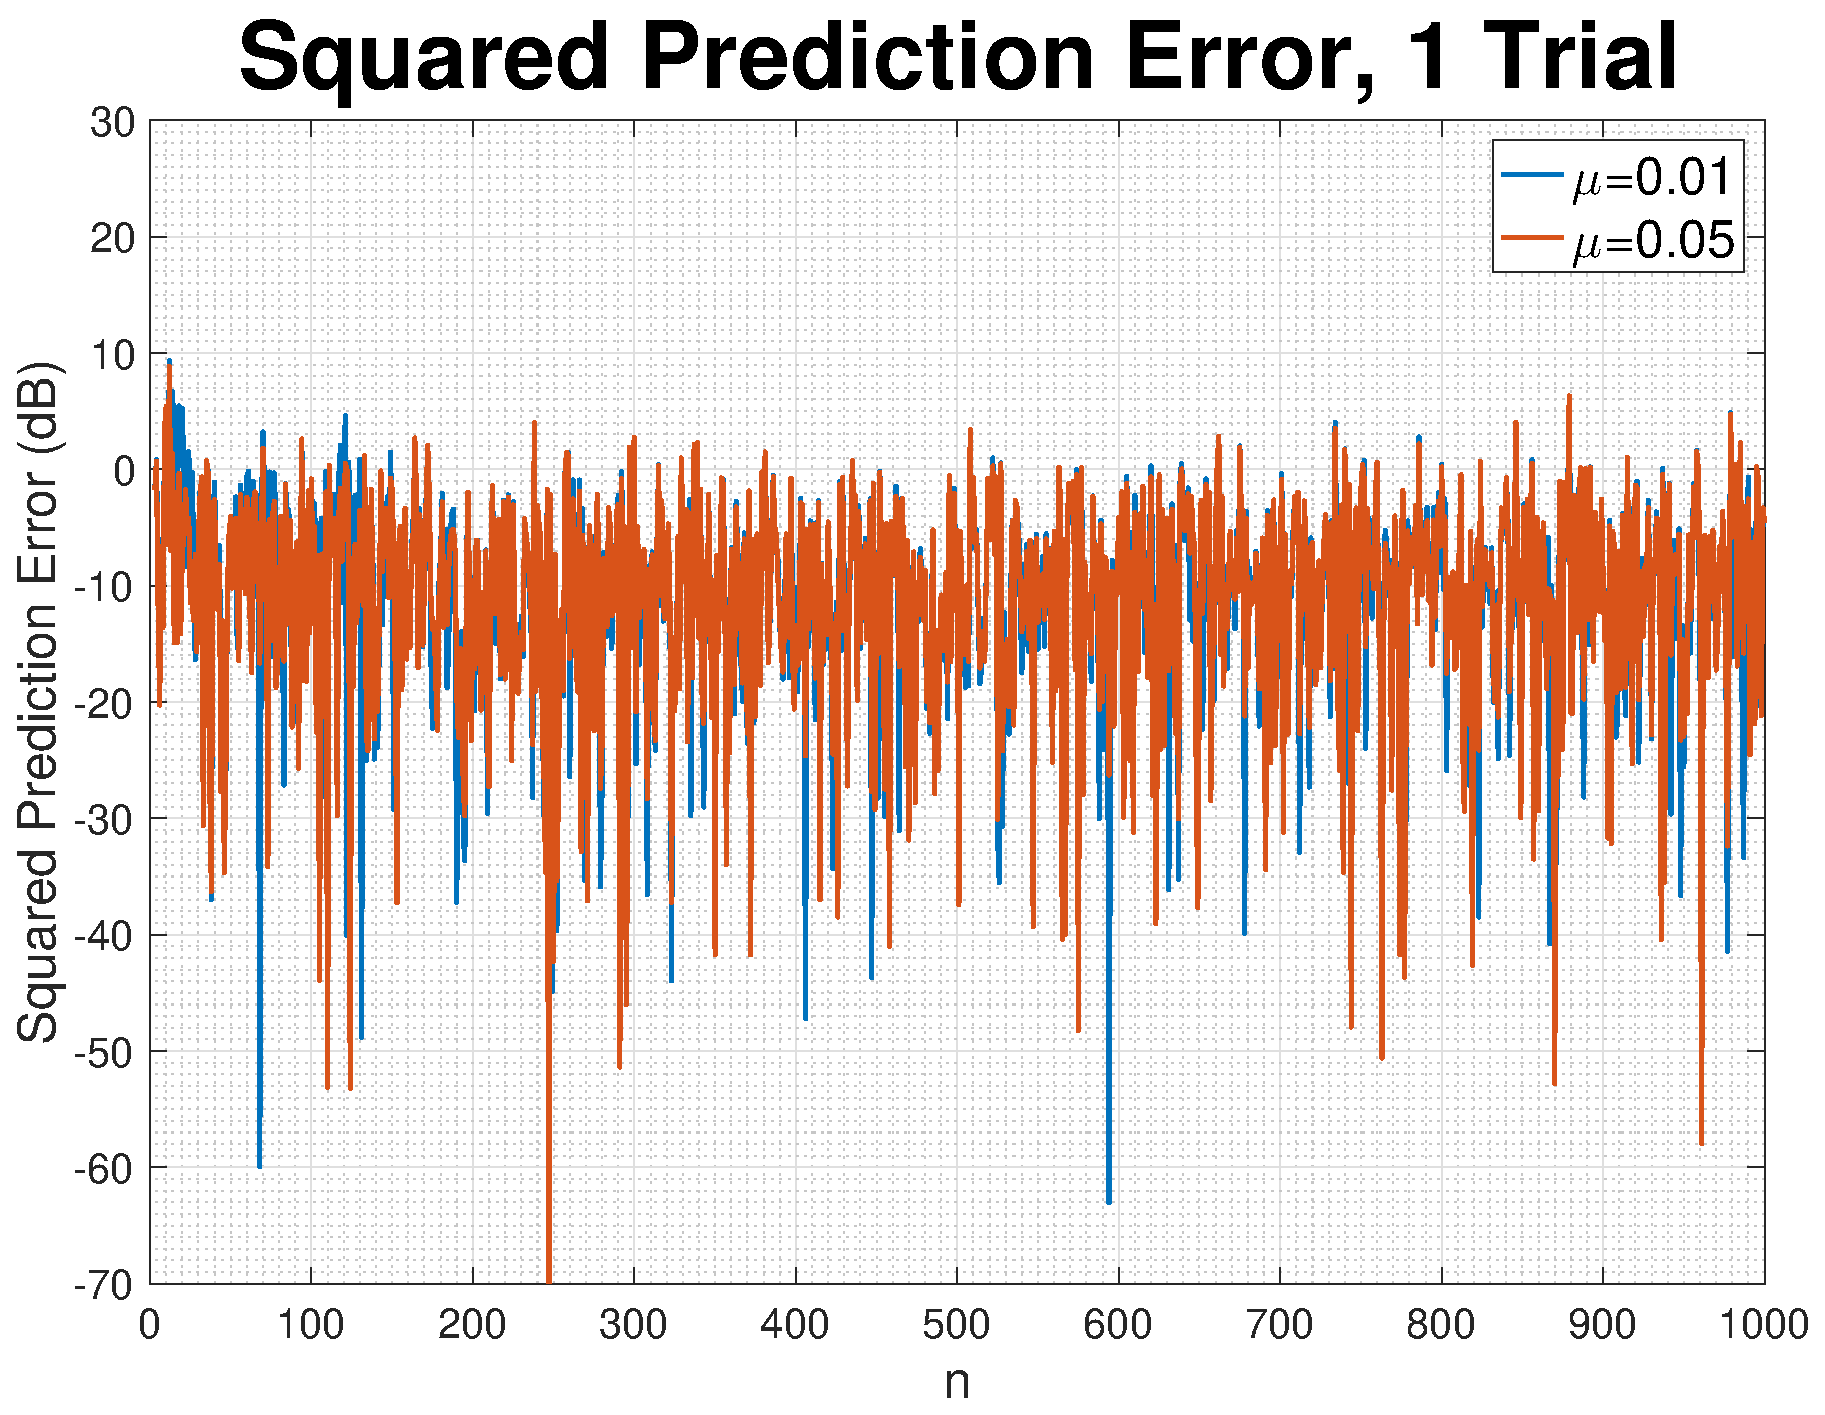
\includegraphics[width=0.32\textwidth]{part3/ar_lms_mu_1_realisation}
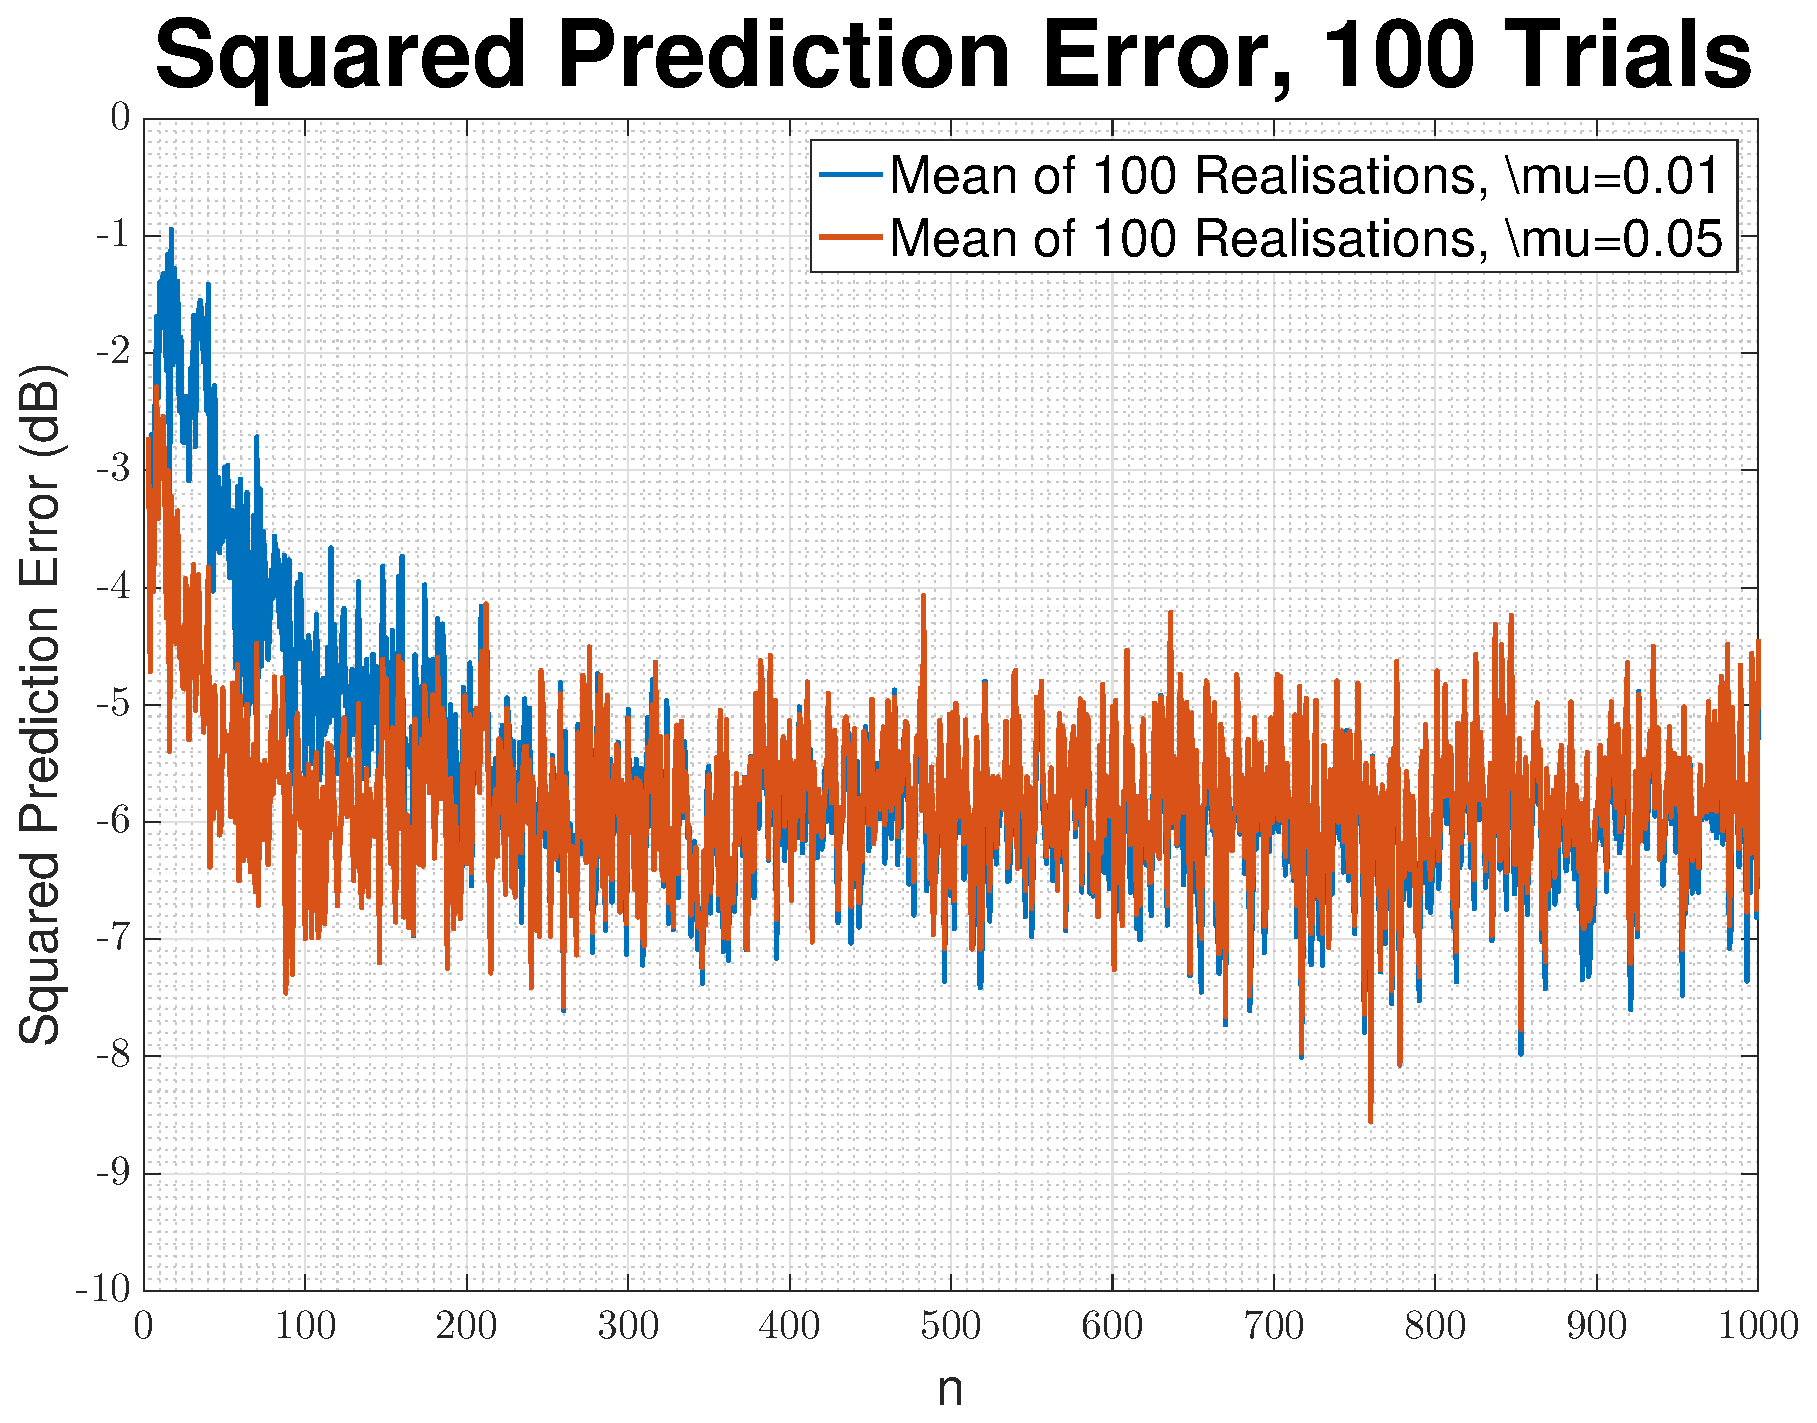
\includegraphics[width=0.32\textwidth]{part3/ar_lms_mu_100_realisation}
\caption{Analysis of Effects of Different Step Size on Convergence Speed of LMS Alogirthm}
\end{figure}

\noindent{}b. The LMS adaptive predictor using $N=1000$ samples of $x(n)$ was implemented. Results of 1 realization and the average of 100 realizations are shown in the figure above for $\mu=0.01$ and $\mu=0.05$. Looked at the squared prediction error, it is clear that on average we obtain faster convergence when $\mu=0.05$. This is exactly as expected as a larger value of $\mu$ would allow the algorithm to decent down the error at a faster rate.

\begin{figure}[H]
\centering{}
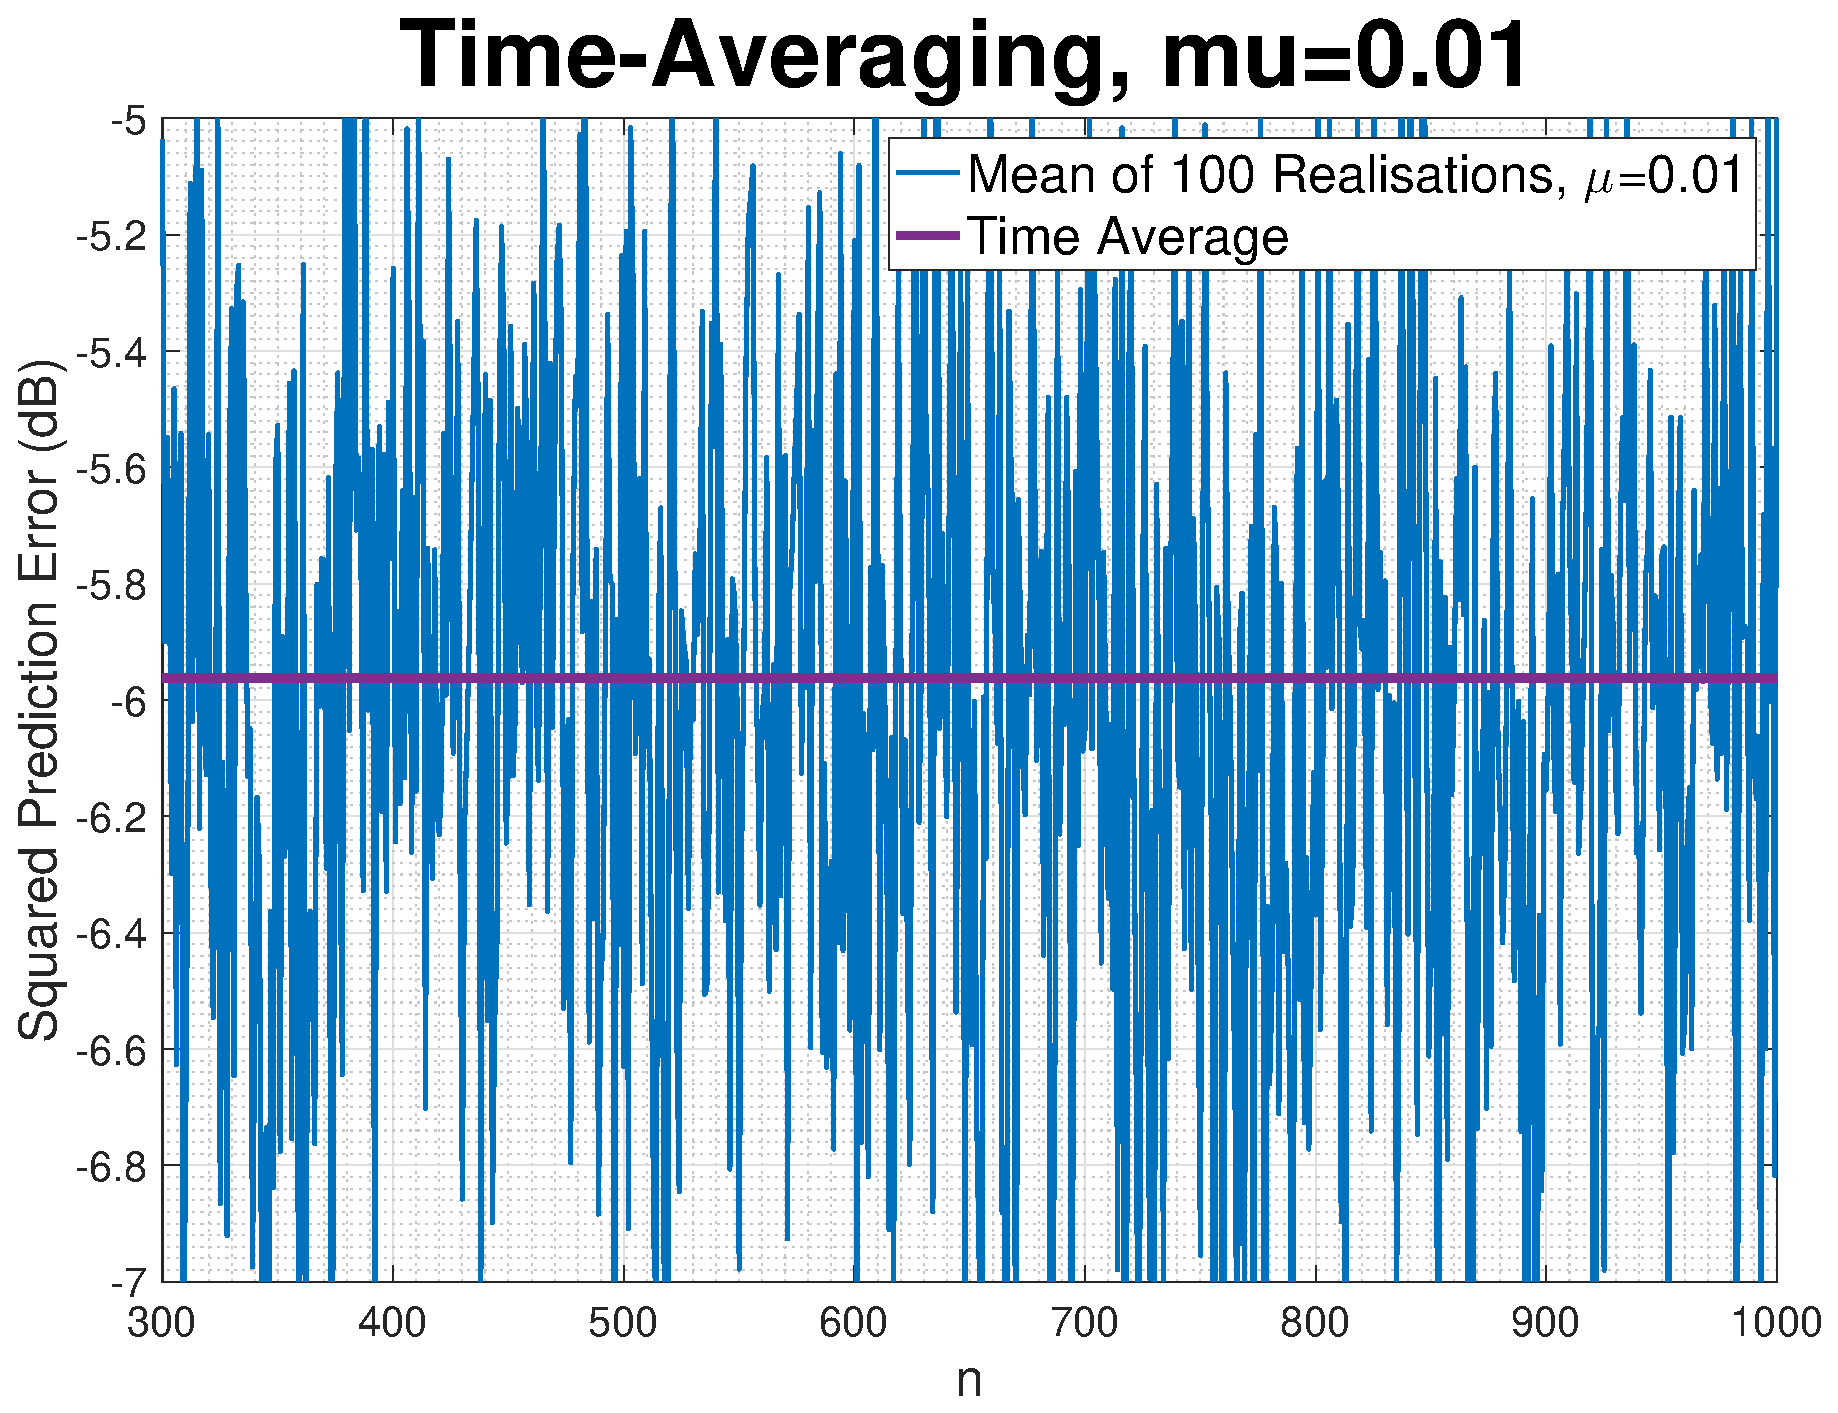
\includegraphics[width=0.32\textwidth]{part3/time_average_mu_01}
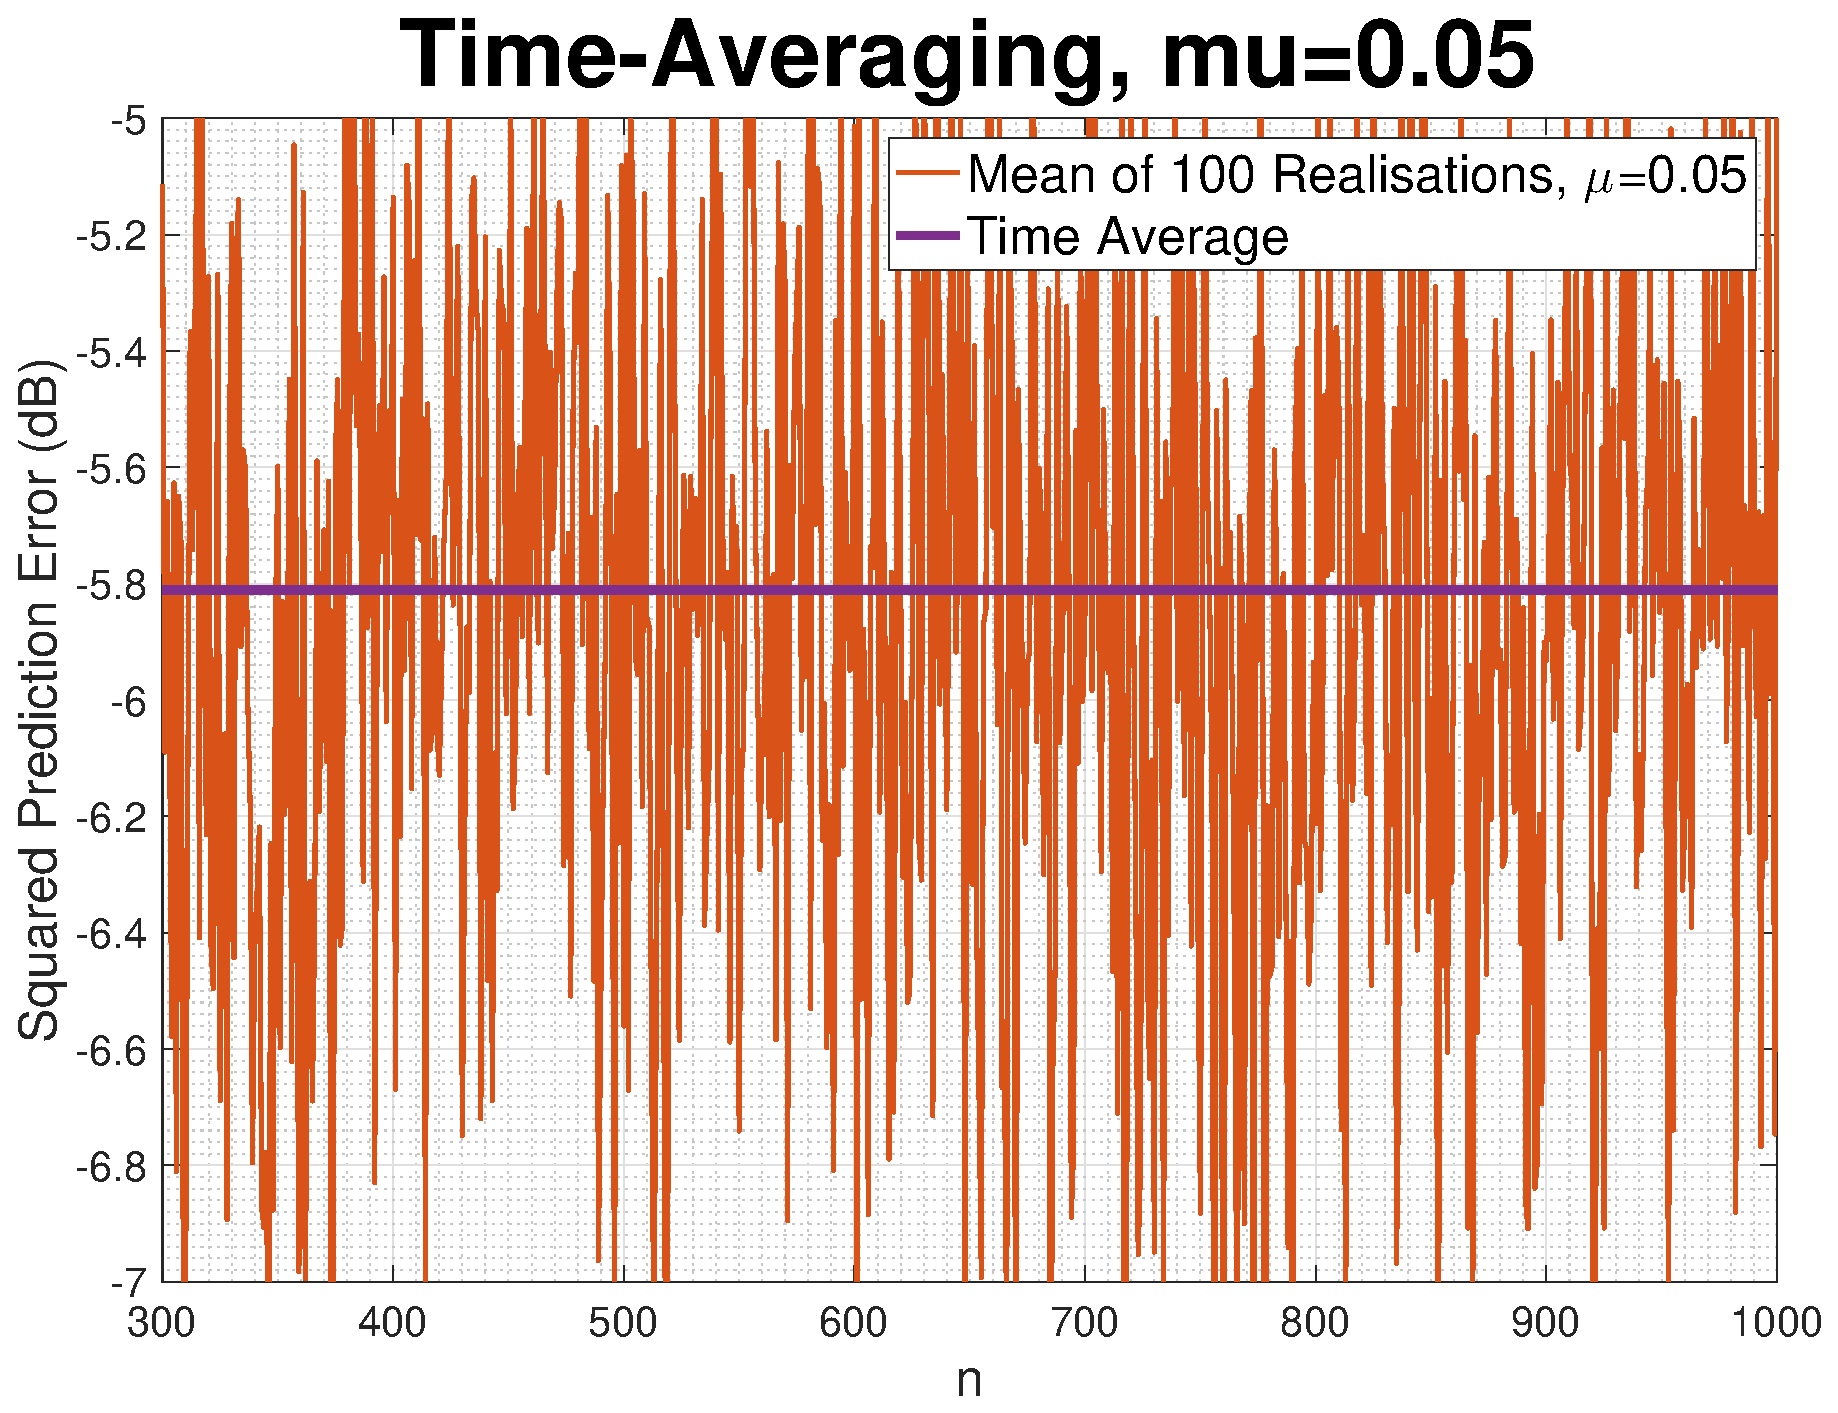
\includegraphics[width=0.32\textwidth]{part3/time_average_mu_05}
\caption{Time-Average of Steady State Error for $\mu=0.01$ and $\mu=0.05$}
\end{figure}


\noindent{}c. The figure above shows the steady-state of the ensemble-average learning curves using 100 independent trials of the experiment. Based on the 100 independent realizations, the excess mean square error, misadjustment and theoretical misadjustment are calculated and the results are shown in the table below. The empirical misadjustment are slightly higher than the theoretical values. Regardless, it is abundantly clear that having a smaller step size introduces a much smaller excess mean square error and results in a smaller misadjustment value. However, as observed above, having a smaller step size causes the rate of convergence to be slow.  

\begin{table}[H]
\centering
\label{my-label}
\begin{tabular}{|c|c|c|c|c|}
\hline
mu   & EMSE   & Empirical Misadjustment 	& Theoretical Misadjustment		\\ \hline
0.01 & 0.0032 & 0.0128                 	& 0.0093                   		\\ \hline
0.05 & 0.124  & 0.0496                 	& 0.0463                  		\\ \hline
\end{tabular}
\end{table}

\noindent{}d. The graphs below show how the coefficients evolve over time. For the rest of the section, most graphs will show the evolution of coefficients, averaged over 100 realizations, and thus it is good to get a feel of what the graphs look like for just 1 realization. Real world adaptive filters will more often than not only work with 1 realization of a random signal. Looking more specifically at the evolution of coefficients for $\mu=0.05$ for 1 realization, it is clear that speed has been traded off for steady-state error. The amount of variation around the ideal values is significant.

\begin{figure}[H]
\centering{}
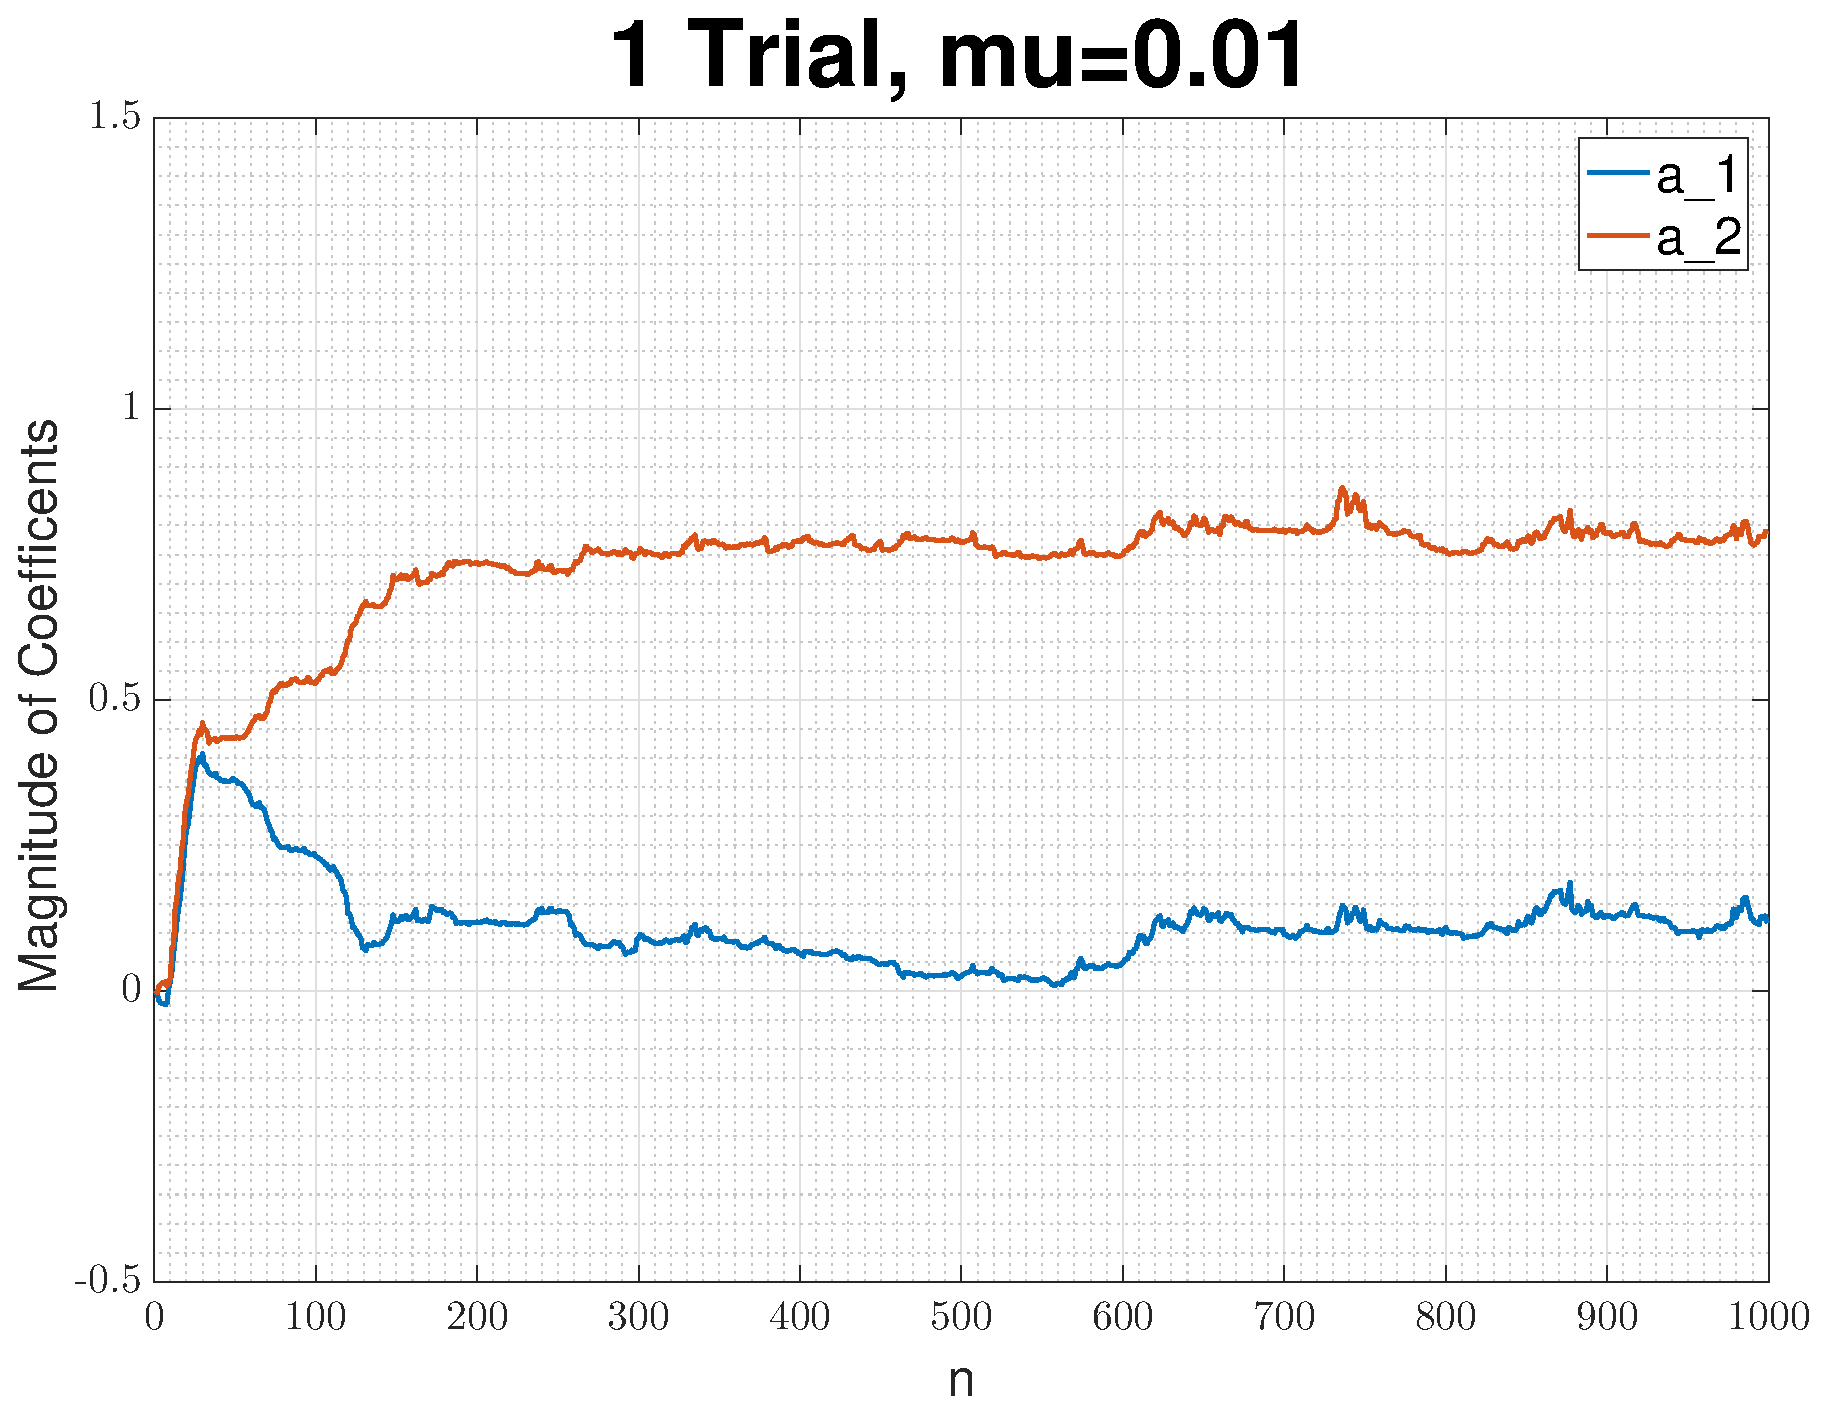
\includegraphics[width=0.32\textwidth]{part3/ar_coefficients_evolution_mu_01_1_trial}
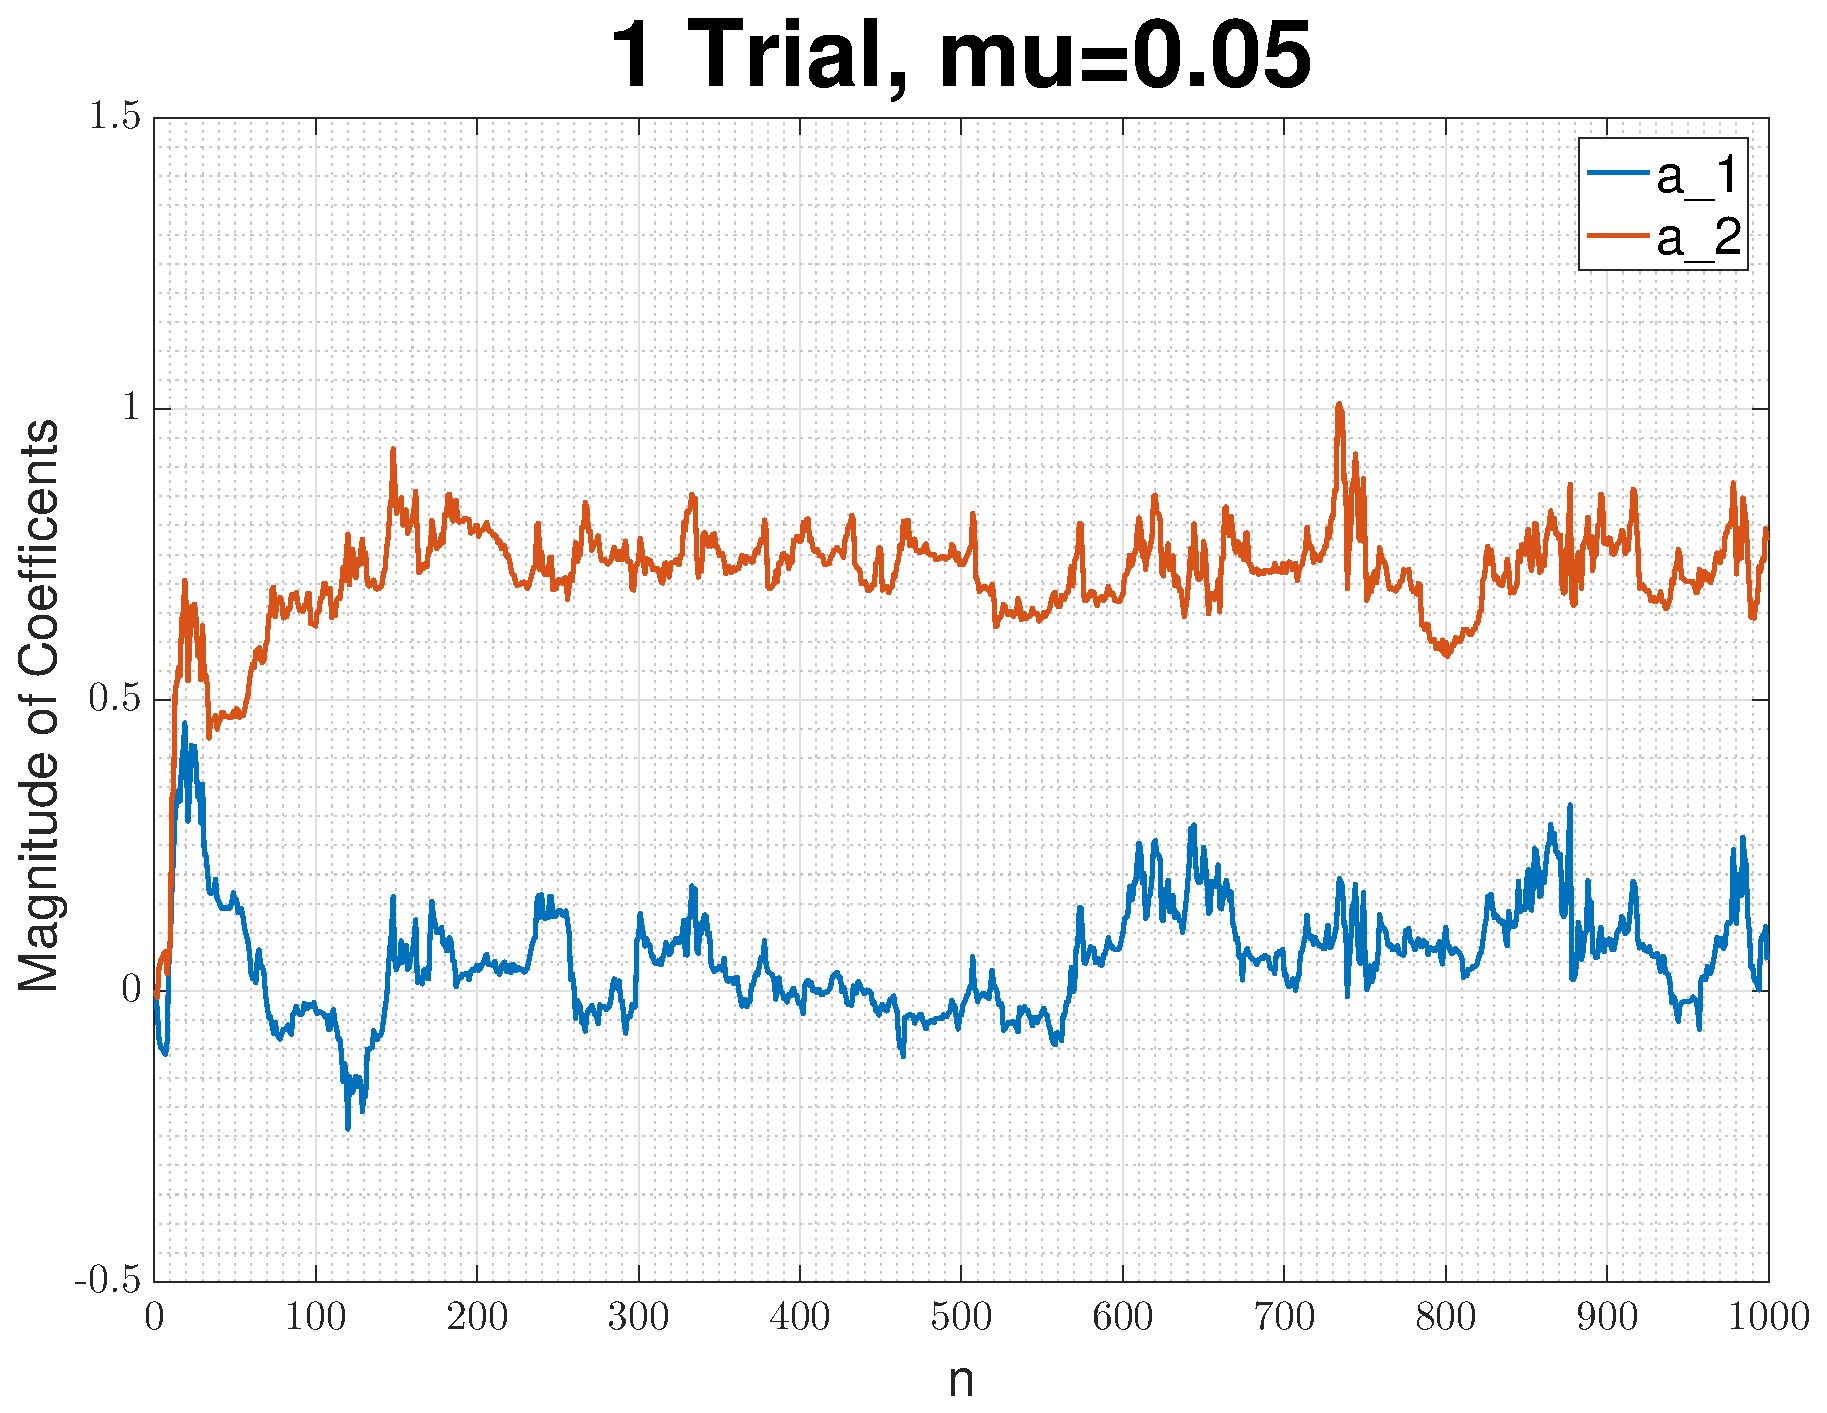
\includegraphics[width=0.32\textwidth]{part3/ar_coefficients_evolution_mu_05_1_trial} \\ 
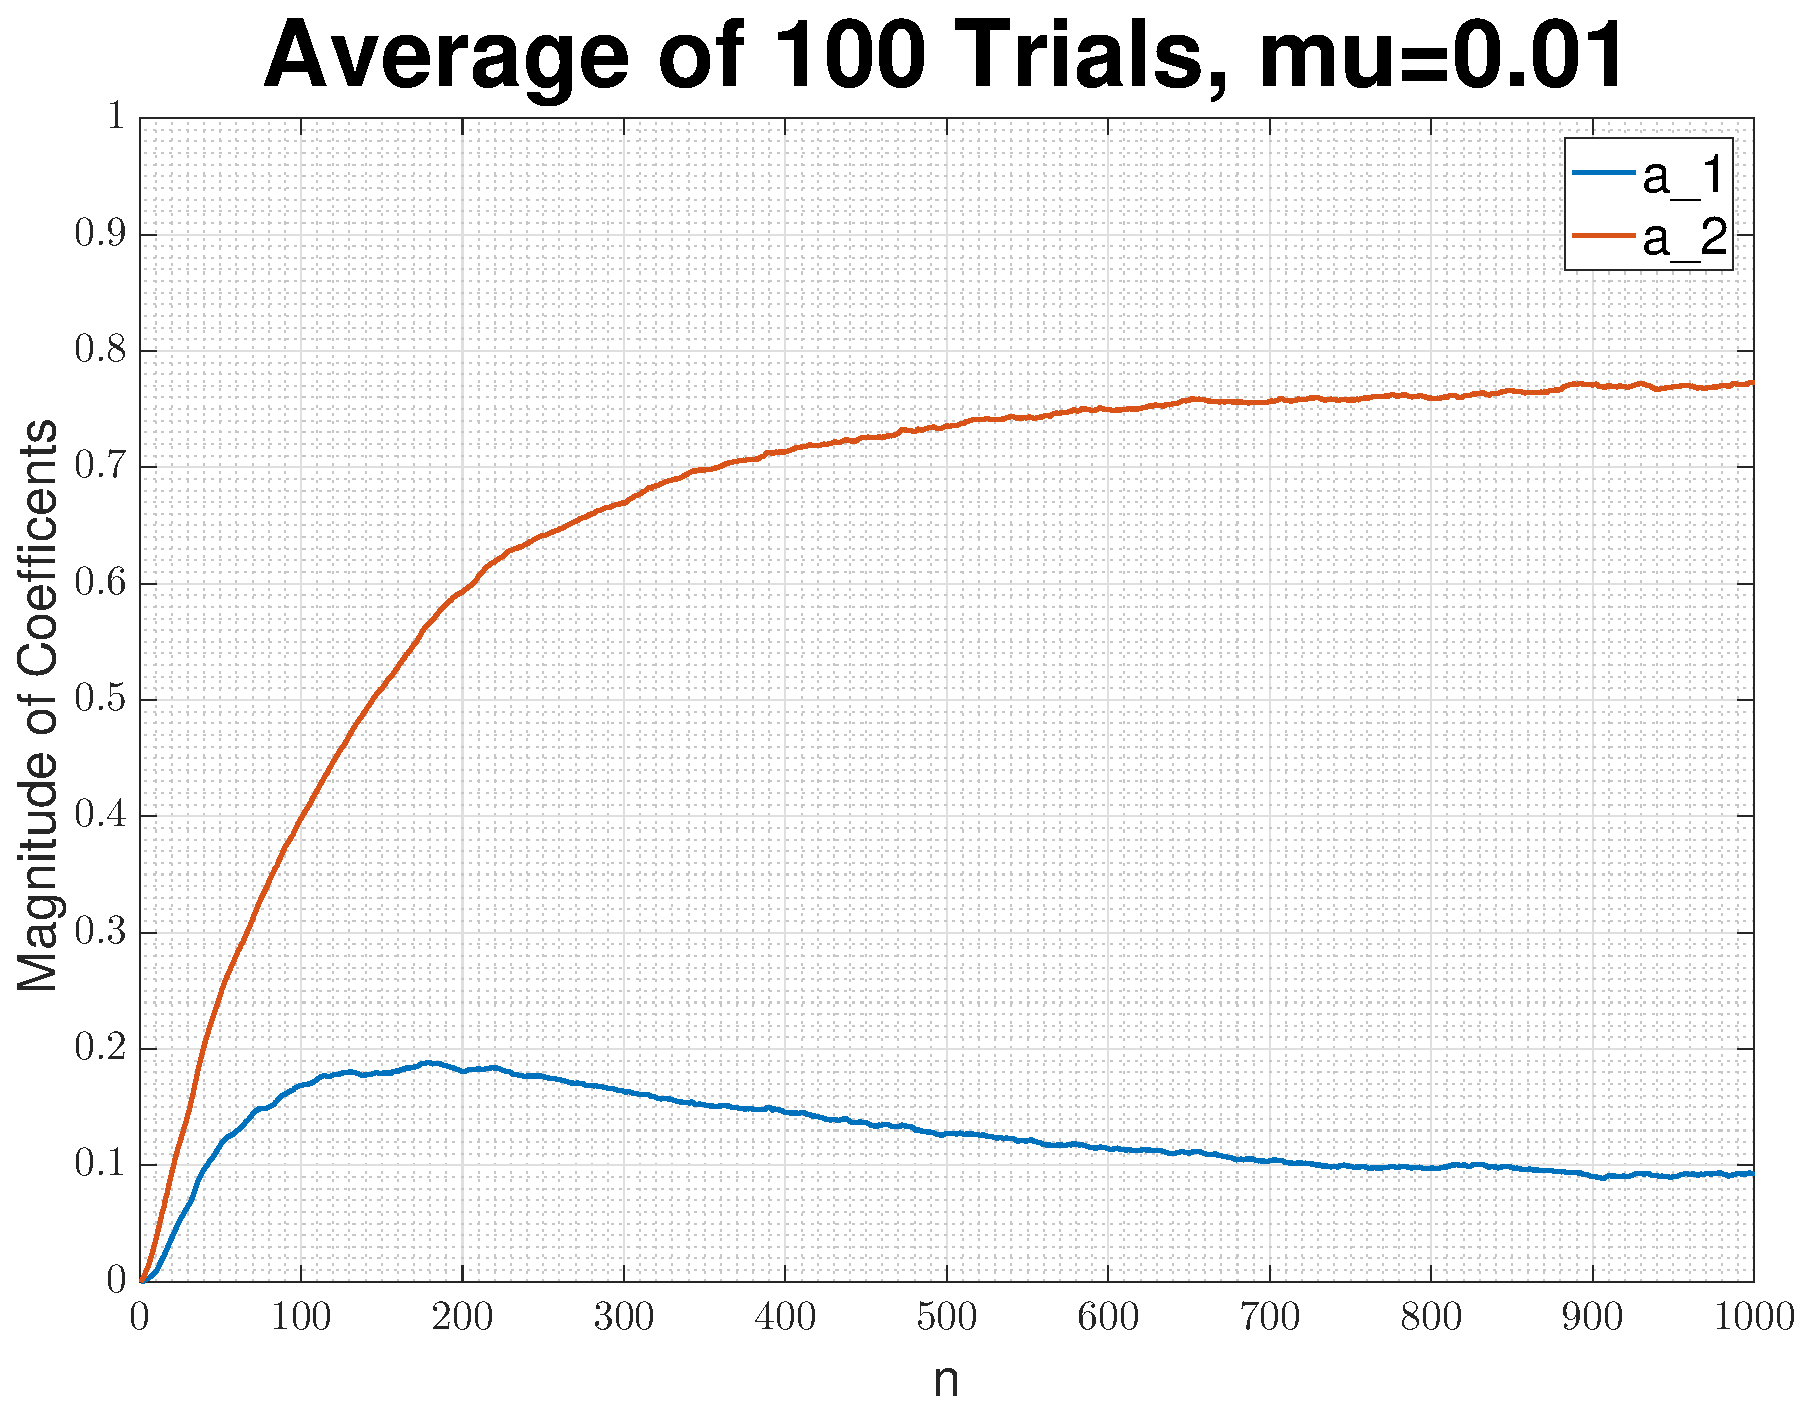
\includegraphics[width=0.32\textwidth]{part3/ar_coefficients_evolution_mu_01}
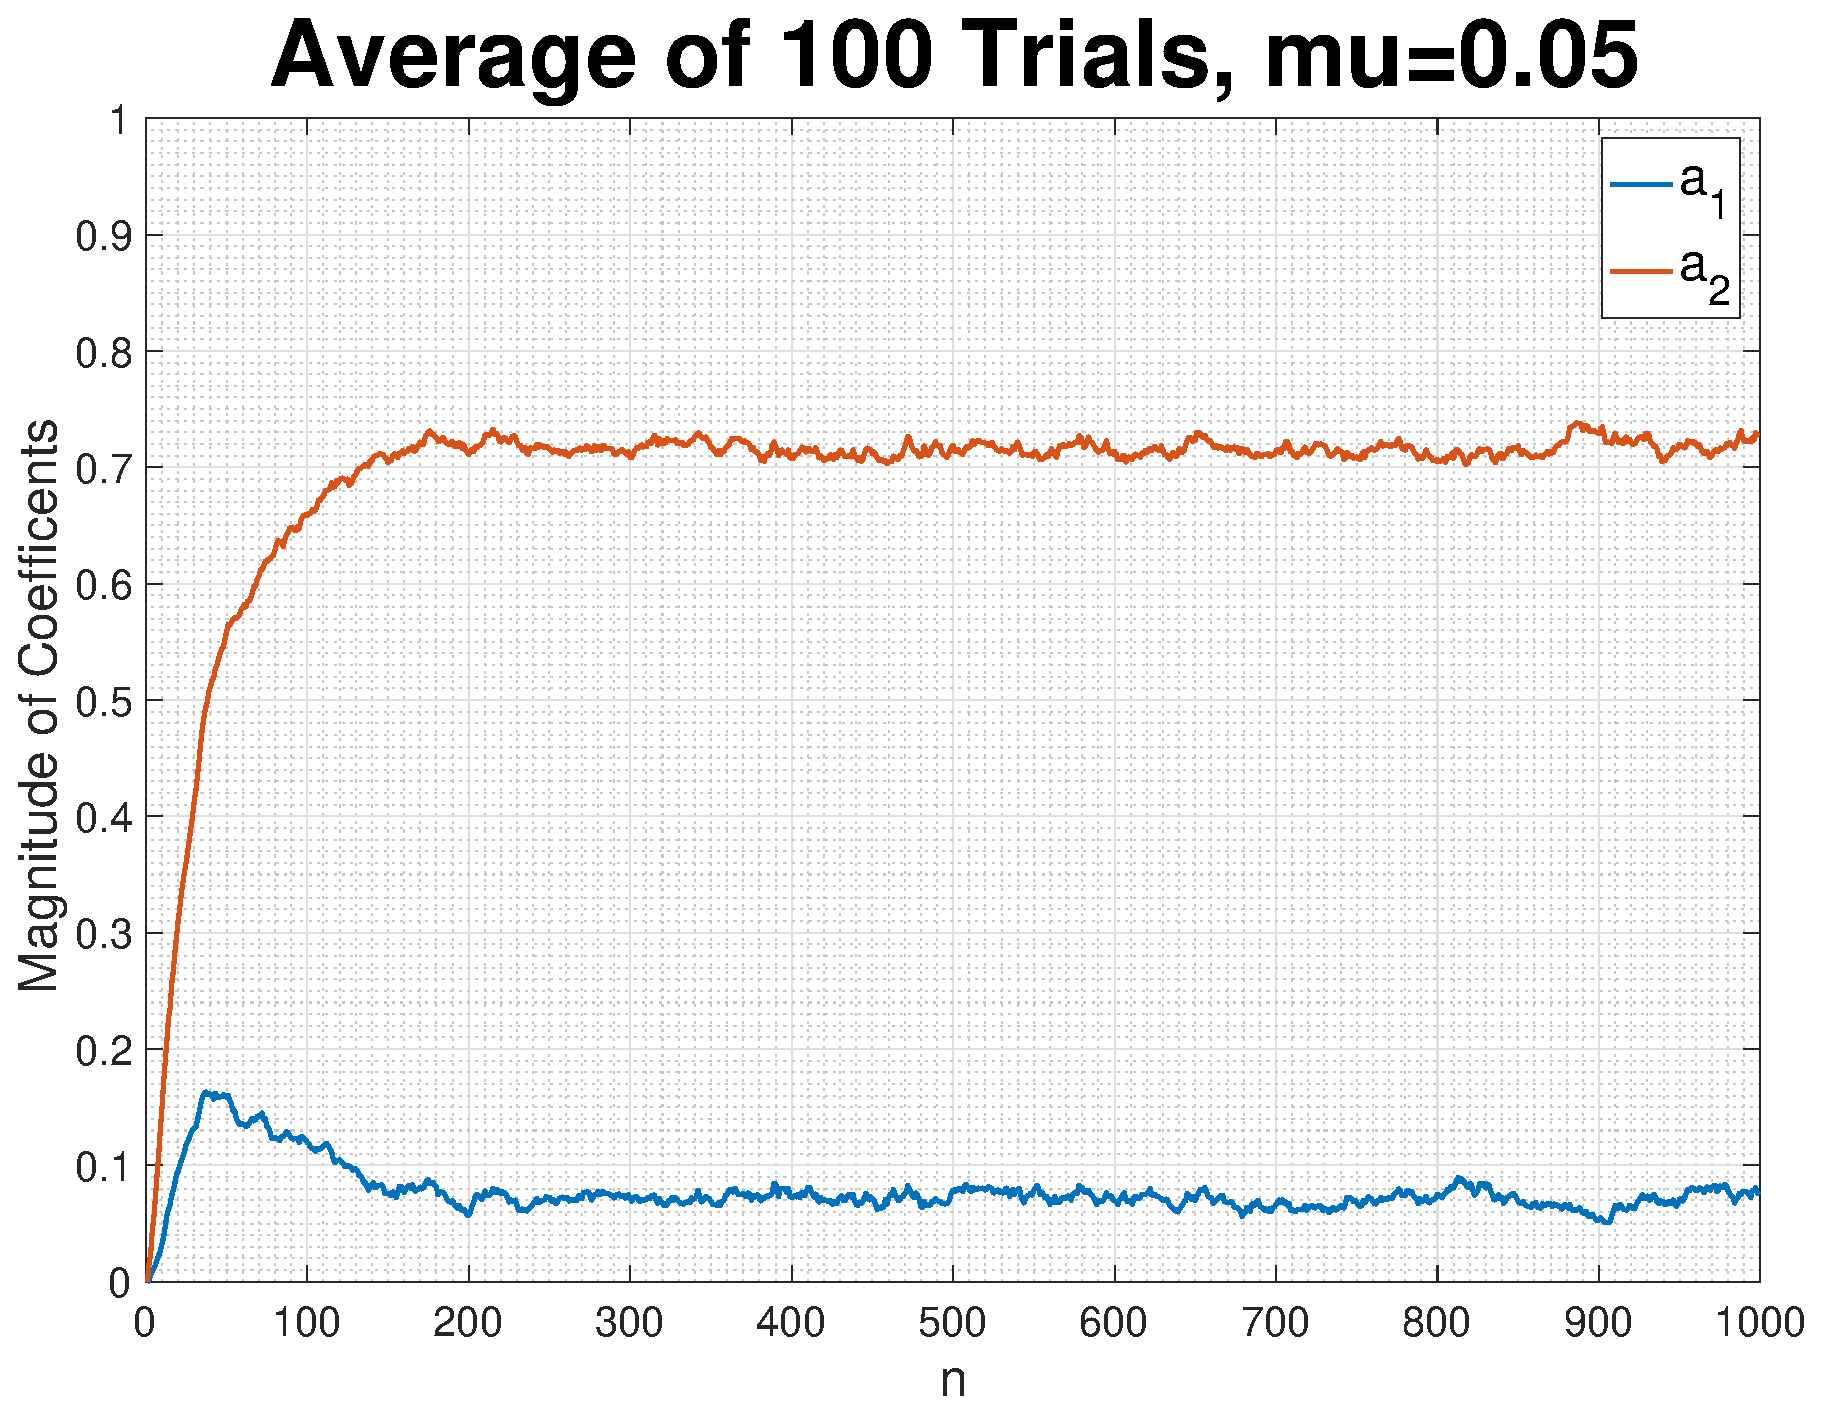
\includegraphics[width=0.32\textwidth]{part3/ar_coefficients_evolution_mu_05}
\caption{Evolution of Coefficients for 1 Trial and 100 Trial, for $\mu=0.01$ and $\mu=0.05$}
\label{fig:steady_state_convergence}
\end{figure}

\noindent{}Next, to answer the question directly, we observe Figure \ref{fig:steady_state_AR}. It is clear that for both coefficients, having a small value of $\mu$ results in the steady state value that is much closer to the ideal values of $a_1=0.1$ and $a_2=0.8$. In addition, having a small value of $\mu$ results in a much smaller steady-state variance. However, looking at Figure \ref{fig:steady_state_convergence}, we find that setting $\mu=0.01$, we do not approach the steady state value until the 900th iteration. In contrast, using $\mu=0.05$, the algorithm converges in about 200 iterations.

\begin{figure}[H]
\centering{}
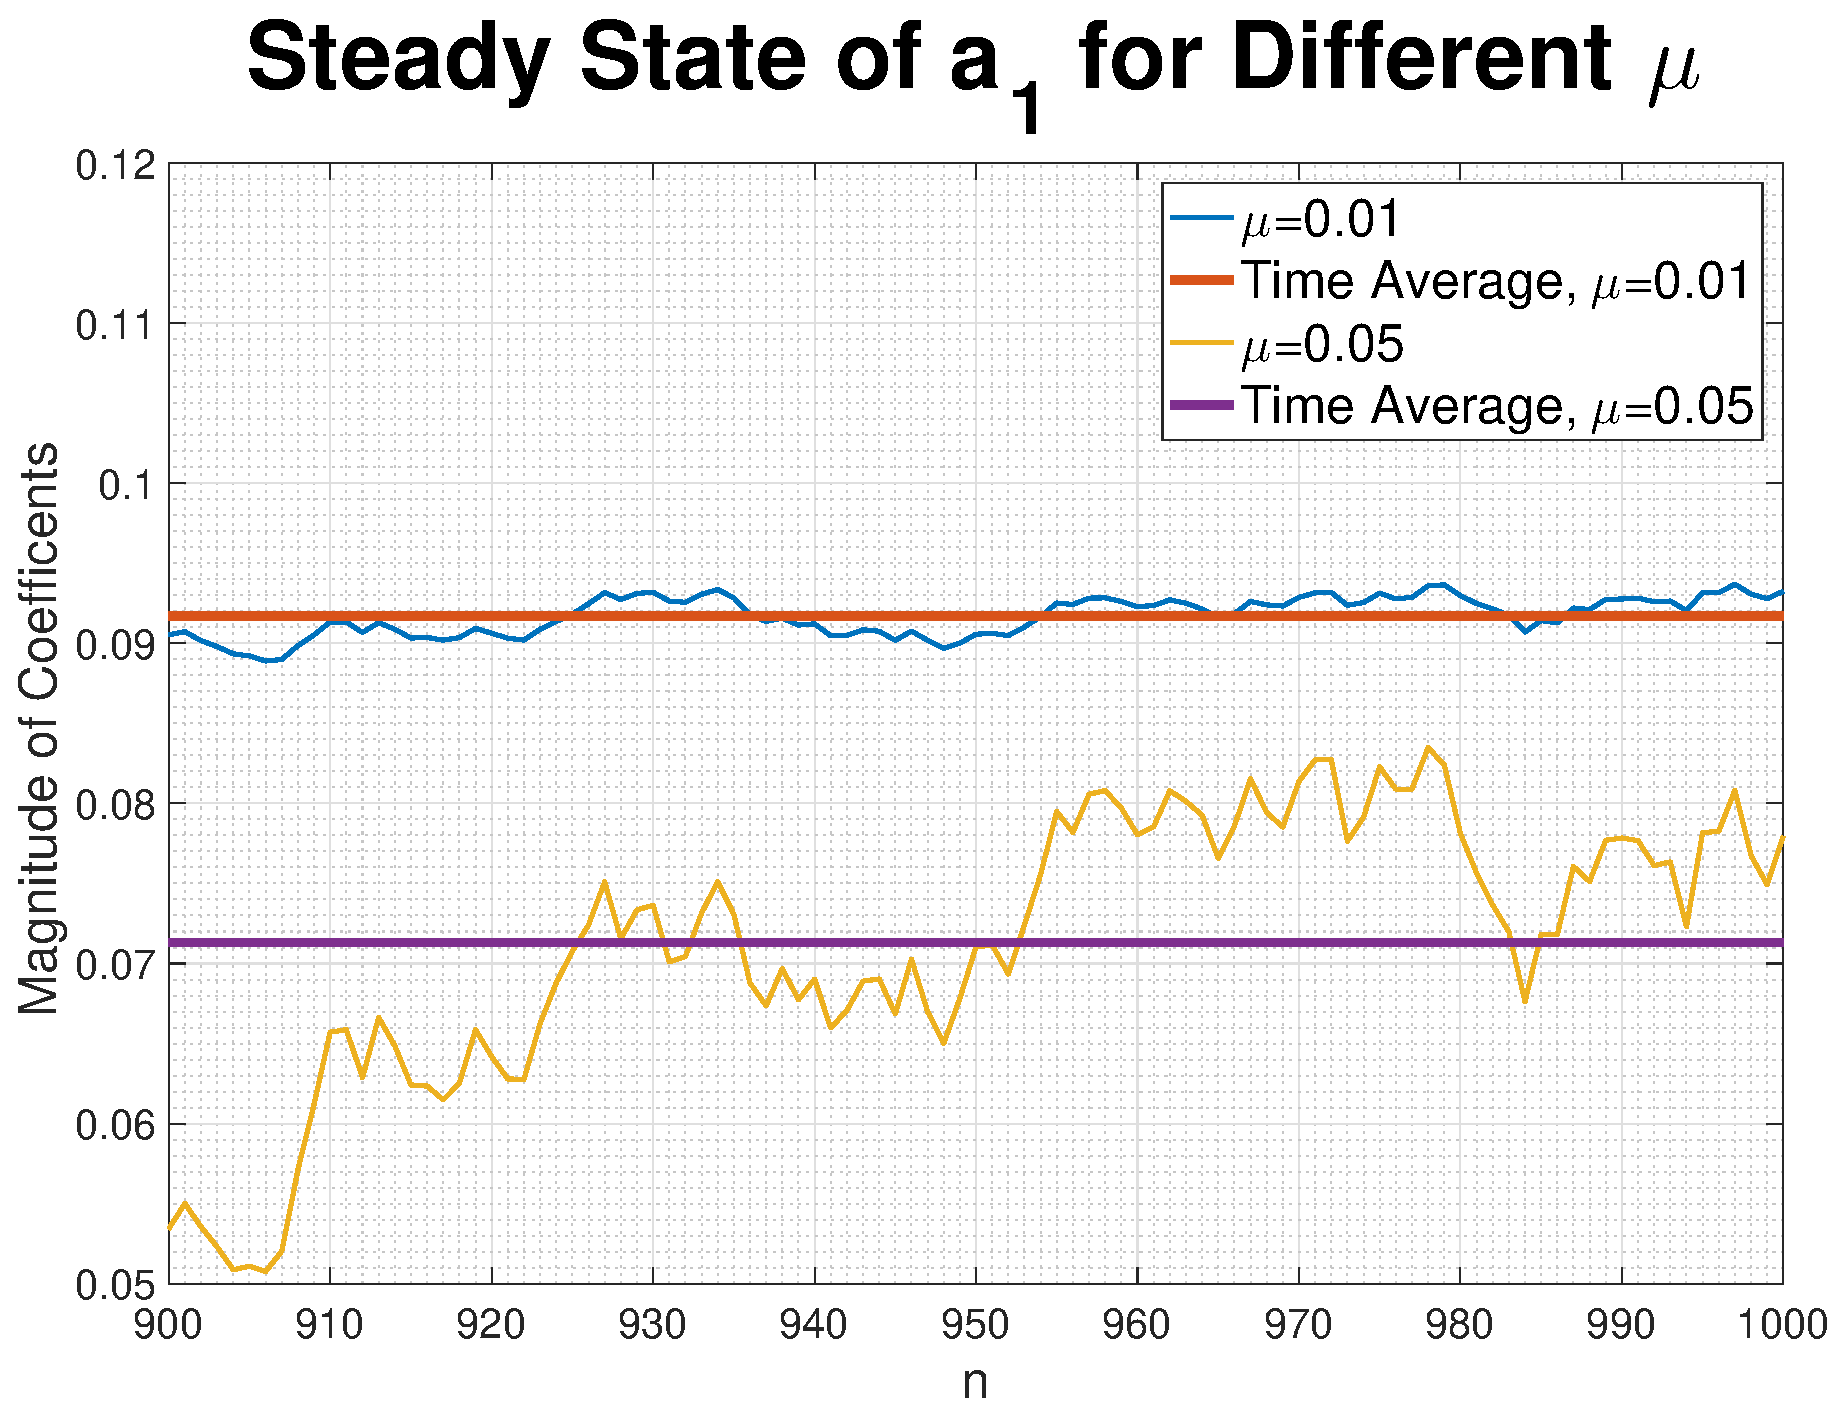
\includegraphics[width=0.32\textwidth]{part3/steady_state_ar_coeff_1}
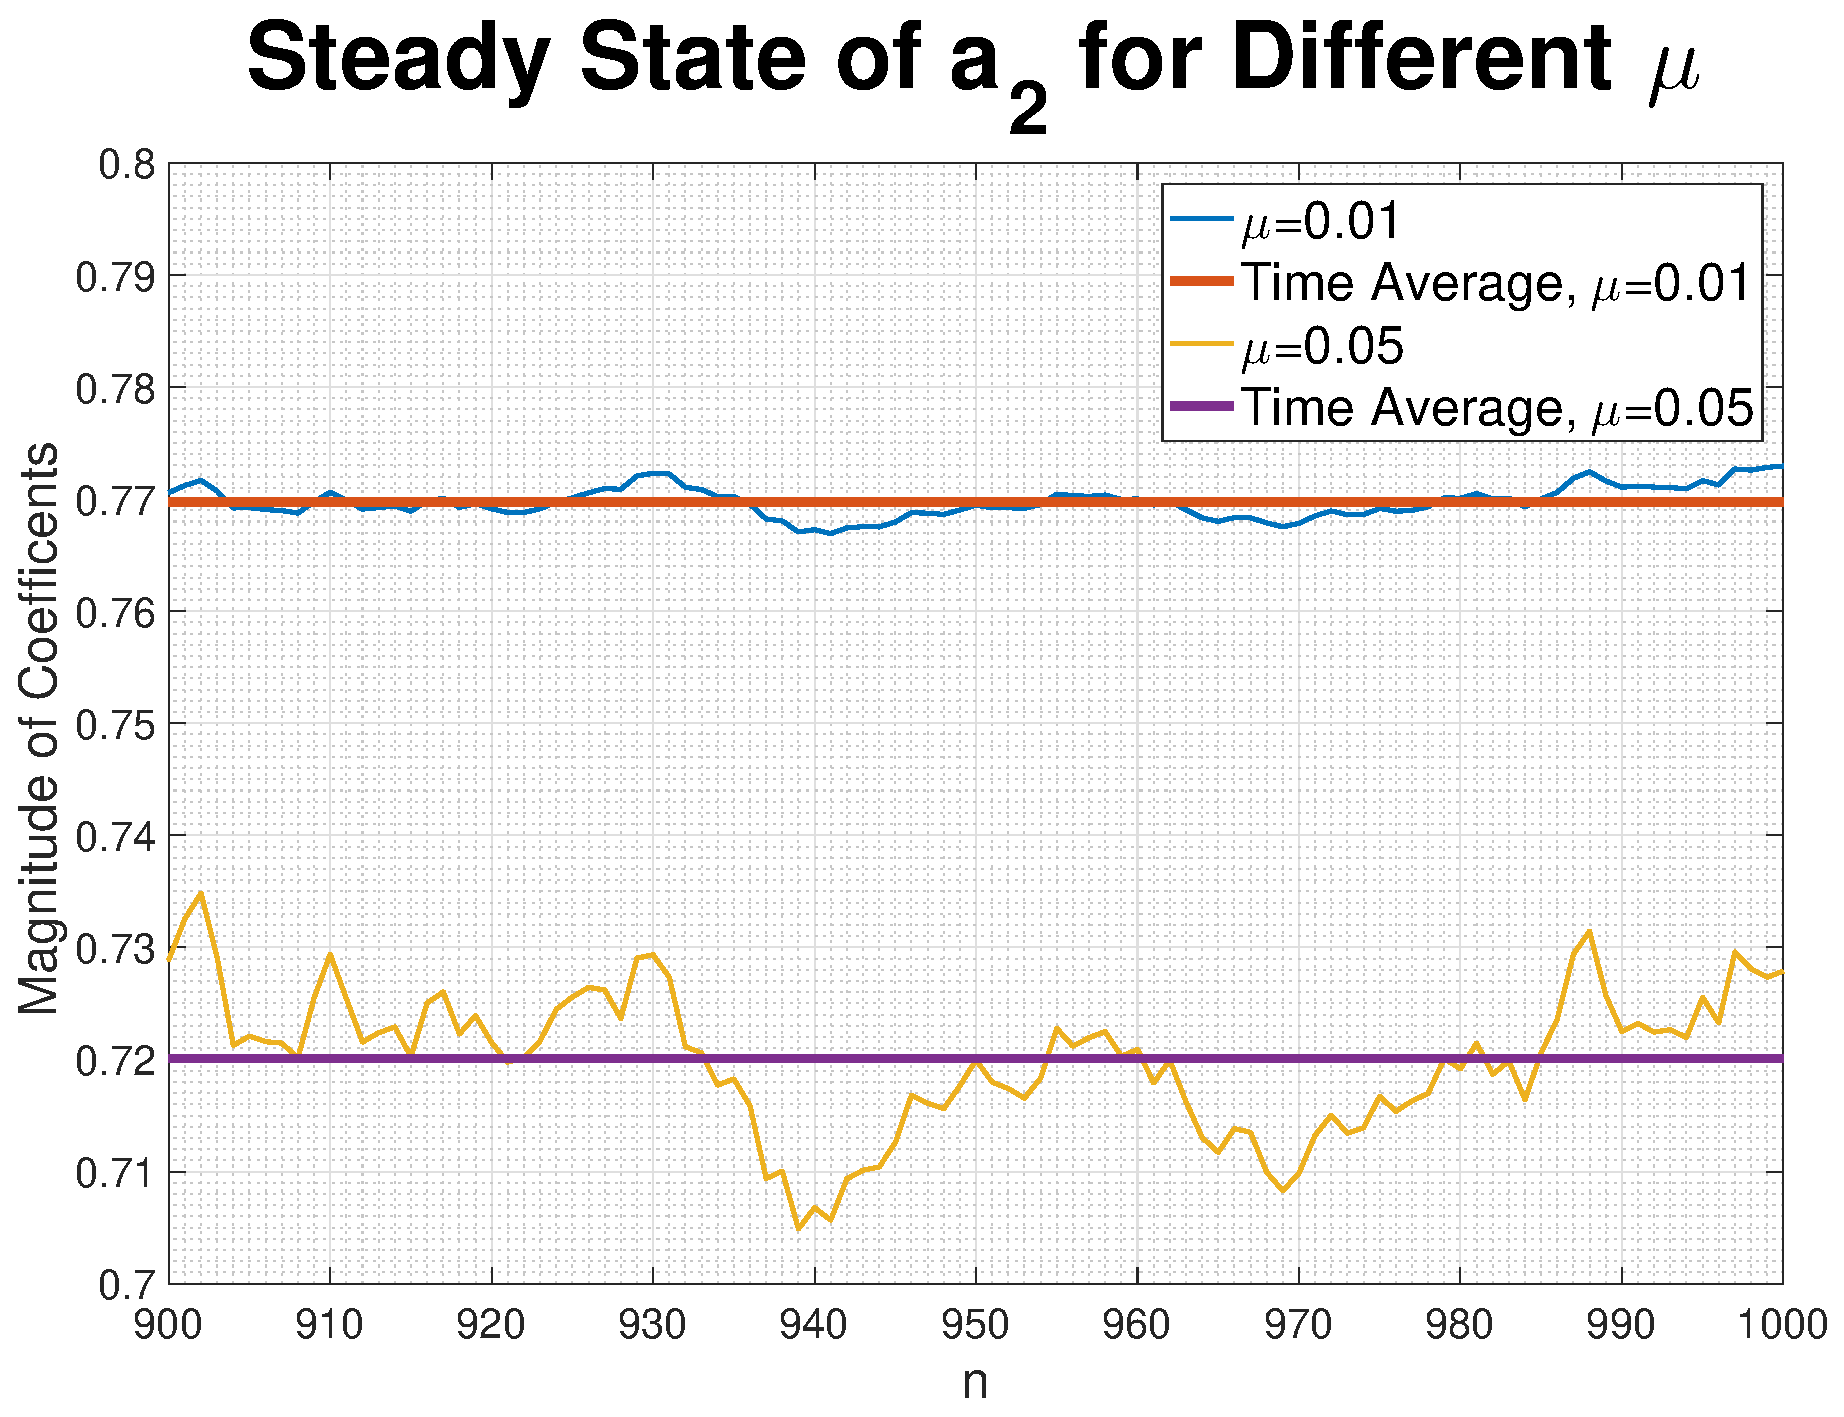
\includegraphics[width=0.32\textwidth]{part3/steady_state_ar_coeff_2}
\caption{Steady State Values of Coefficients $a_1$ and $a_2$, for $\mu=0.01$ and $\mu=0.05$}
\label{fig:steady_state_AR}
\end{figure}

\noindent{}e. In order to minimize the cost function, we differentiate it and set the derivative to 0. Mathematically, we obtain:

\begin{align}
J(n) &= \frac{1}{2}\Bigg(e^2(n)+\gamma||\textbf{w}(n)||^2\Bigg) \label{eq:cost_func}\\ 
\frac{\partial J}{\partial \textbf{w}} &= e(n)\frac{\partial e}{\partial \textbf{w}} + \gamma \textbf{w}(n) = 0 \nonumber
\end{align}

\noindent{}Since,

\begin{align*}
\frac{\partial e}{\partial \textbf{w}} = \frac{\partial}{\partial \textbf{w}}\Bigg(\textbf{x}(n) - \textbf{w}^T(n)\textbf{x}(n)\Bigg) = -\textbf{x}(n)
\end{align*}

\noindent{}Then,

\begin{align*}
\frac{\partial J}{\partial \textbf{w}} = -\gamma \textbf{w}(n) + e(n)
\end{align*}

\noindent{}Now, using the gradient decent method to reach the optimal value of $w$, we have to implement (\ref{eq:w_update})

\begin{align}
\textbf{w}(n) = \textbf{w}(n) - \mu \nabla_{w}J(n) \label{eq:w_update}
\end{align}

\noindent{}Substituting the derivative of the cost function, we obtain:

\begin{align}
\textbf{w}(n+1) &= \textbf{w}(n) - \mu \Bigg(-\gamma \textbf{w}(n) + e(n)\Bigg)\textbf{x}(n) \nonumber\\
\textbf{w}(n+1) &= (1-\mu\gamma)\textbf{w}(n) - \mu e(n)\textbf{x}(n) \label{eq:leaky_lms}
\end{align}

\noindent{}Thereby showing that the leaky LMS equation shown in the notes and derived in (\ref{eq:leaky_lms}) is equivalent to minimizing the cost function shown in (\ref{eq:cost_func}).\\

\noindent{}f. The graphs shown in Figure \ref{fig:leaky_lms} show evolution of coefficients for different values of $\mu$ and $\gamma$ using the leaky LMS algorithm. The steady-state values do not converge to the true values of $a_1$ and $a_2$. In fact, the larger the value of $\gamma$, the greater the steady-state bias. The Weiner-Hopf solution was briefly mentioned above. It gives the optimal weights calculated using the autocorrelation matrix, $\textbf{R}$, and the cross correlation vector, $\textbf{p}$:

\begin{align*}
\textbf{w}_{opt} = \textbf{R}^{-1}\textbf{p}
\end{align*}

\noindent{}The LMS, under certain bounds on the value of $\mu$, iteratively arrives at the Weiner-Hopf solution. The motivation of the algorithm is to prevent the inverting the autocorrelation matrix. The leaky LMS however does not converge to the Wiener-Hopf solution. The leaky LMS minimizing a cost function that is slightly different than the cost function that the LMS algorithm minimizes and thus it converges to:

\begin{align*}
\lim_{k \rightarrow \infty} \mathbb{E}[\textbf{w}_{k}] = (\textbf{R} + \gamma\textbf{I})^{-1}\textbf{p}
\end{align*}

\noindent{}The additional, $\gamma\textbf{I}$ term causes a bias that means that the leaky LMS does not actually converge to the Wiener-Hopf solution. In fact, since $\textbf{p} = [\gamma(1), \gamma(2)]^T$, we can mathematically determine the values to which the algorithm converges:

\begin{table}[H]
\centering
\label{my-label}
\begin{tabular}{|c|c|c|}
\hline
$\gamma$ & $a_1$     & $a_2$     \\ \hline
0.1   & 0.1542 & 0.3919 \\ \hline
0.5   & 0.1626 & 0.4992 \\ \hline
0.9   & 0.1319 & 0.7076 \\ \hline
\end{tabular}
\end{table}

\noindent{}Notice that the graphs confirm the theoretical results calculated above. The leaky LMS displays the same properties with regards to $\mu$. A smaller $\mu$ means slower convergence but a smaller steady-state error whereas a larger $\mu$ means faster convergence but a larger steady-state error. 

\begin{figure}[H]
\centering{}
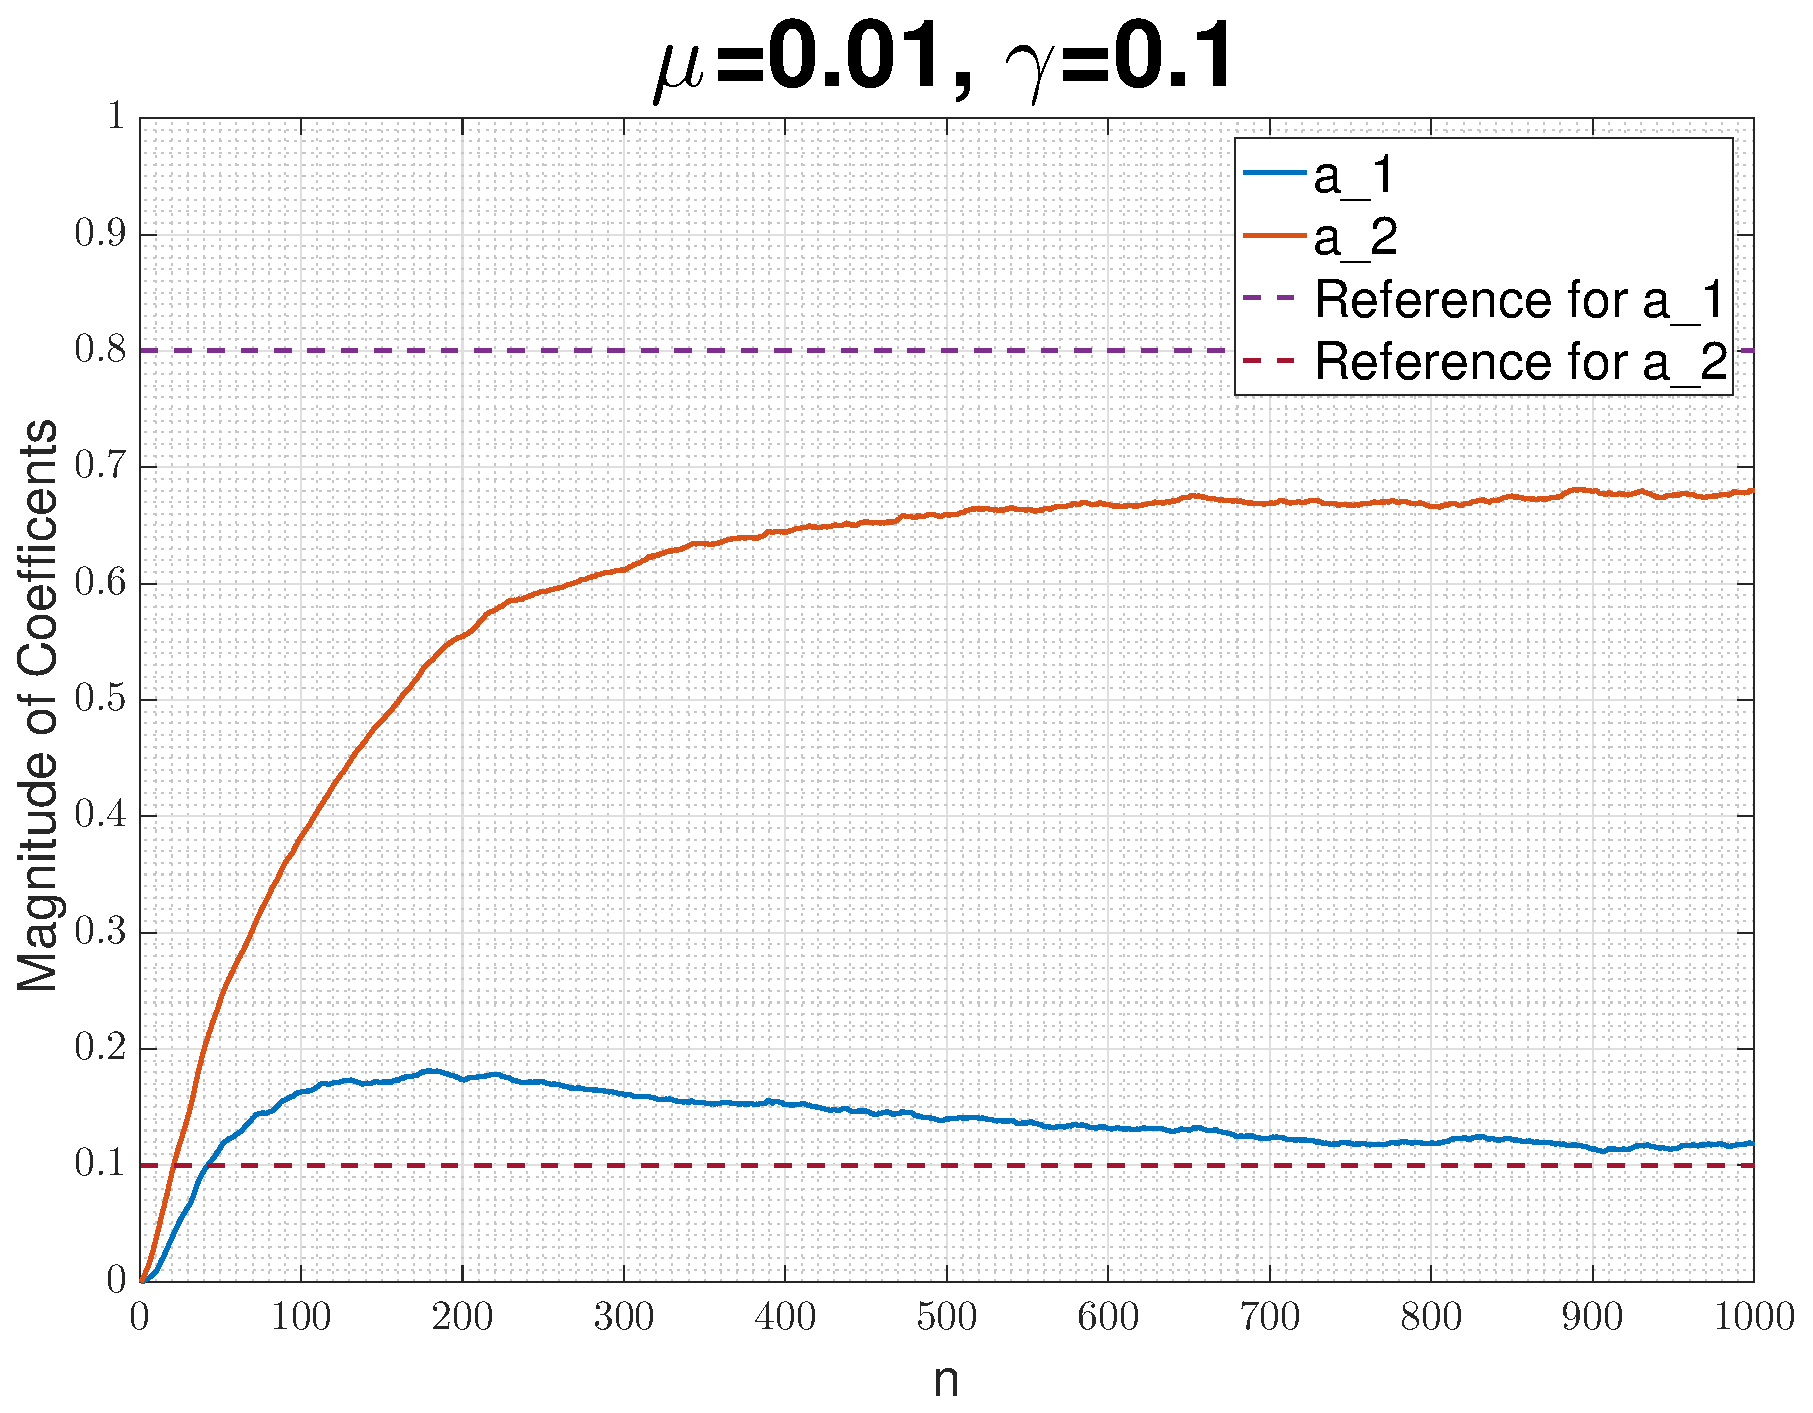
\includegraphics[width=0.32\textwidth]{part3/leaky_mu_01_gamma_01}
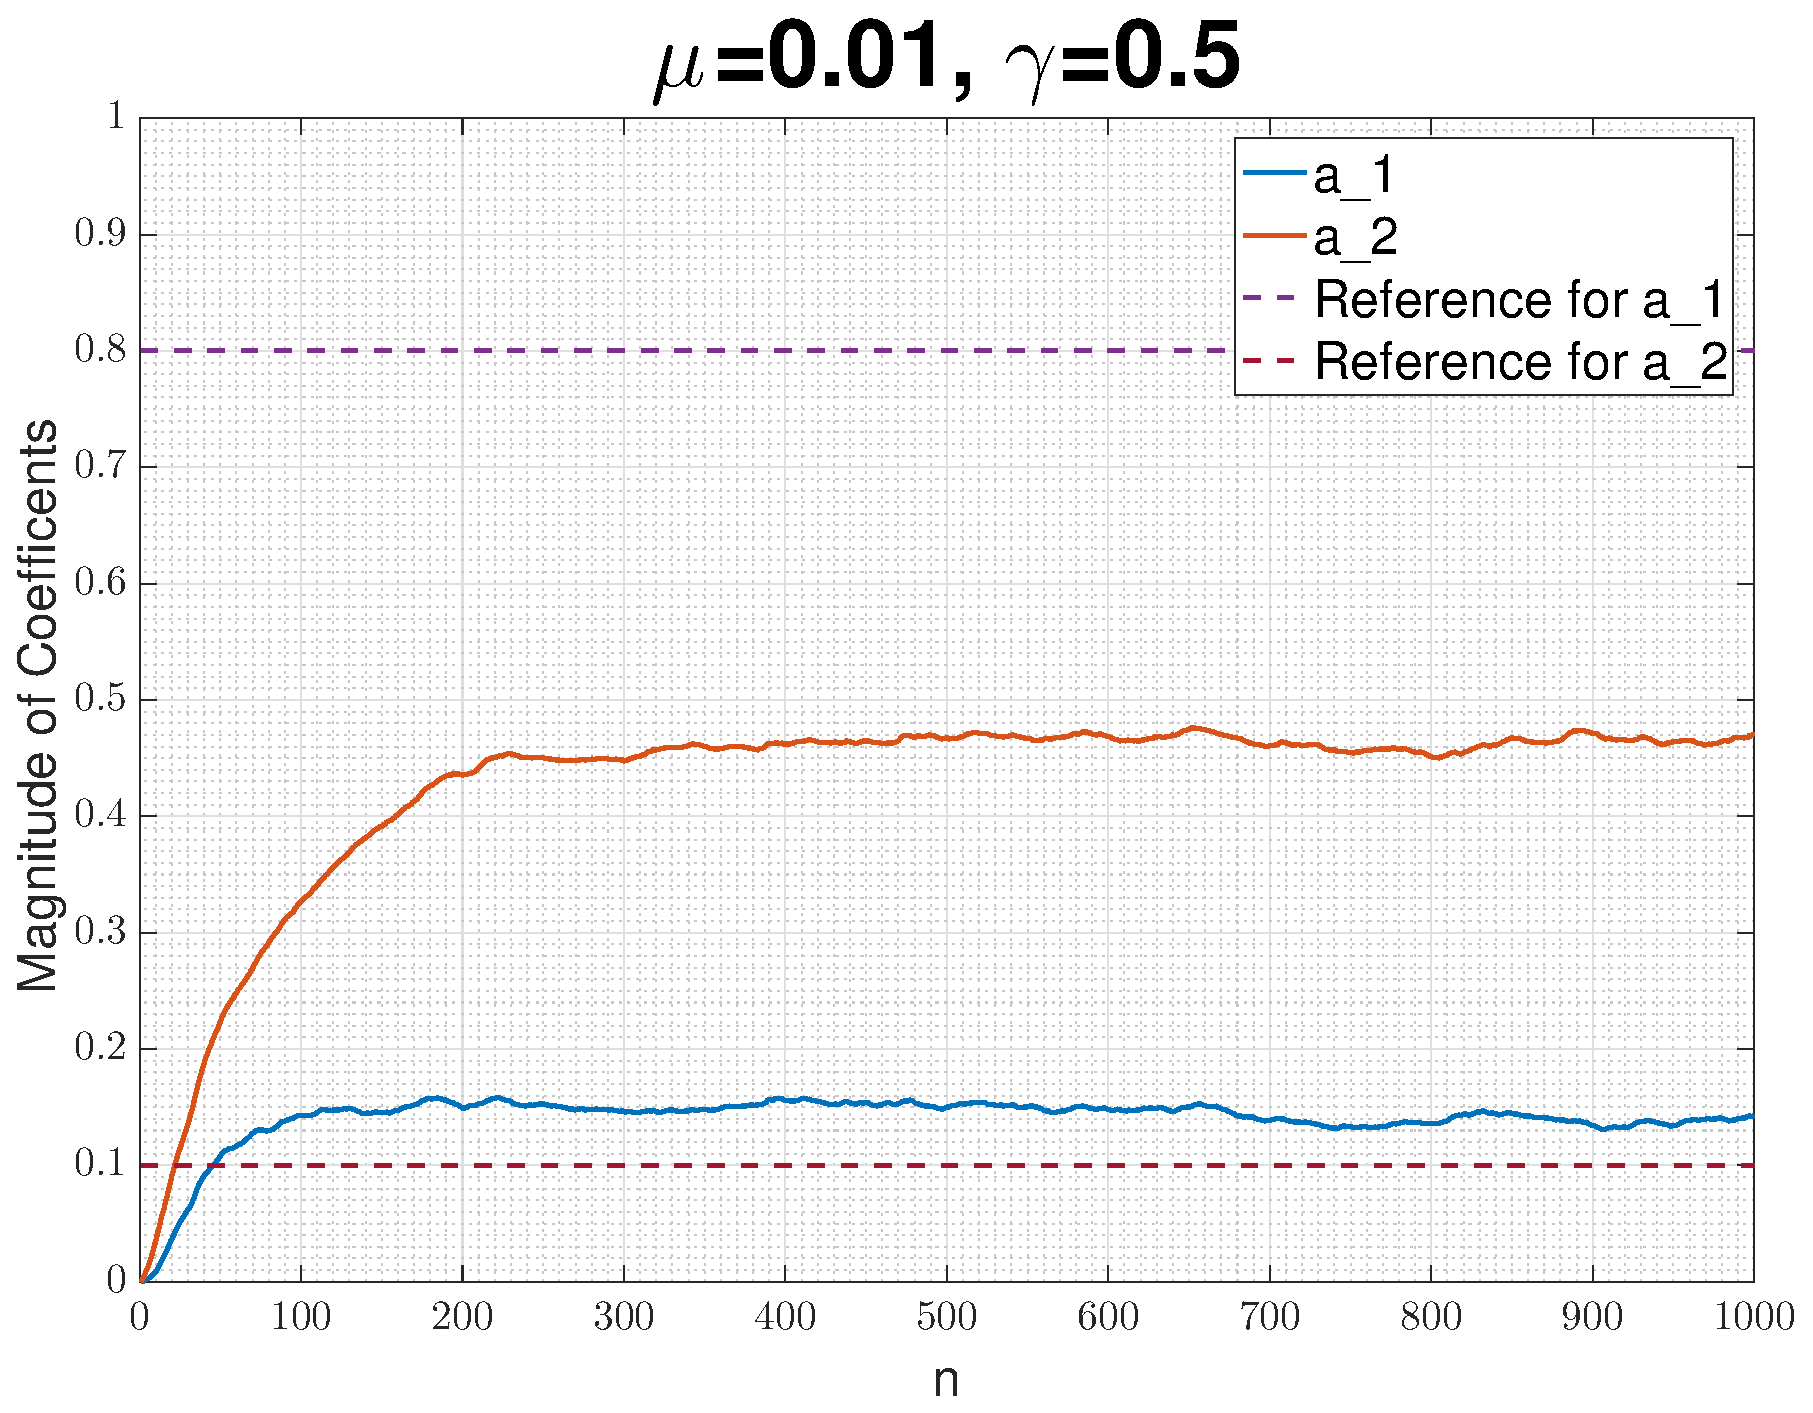
\includegraphics[width=0.32\textwidth]{part3/leaky_mu_01_gamma_05}
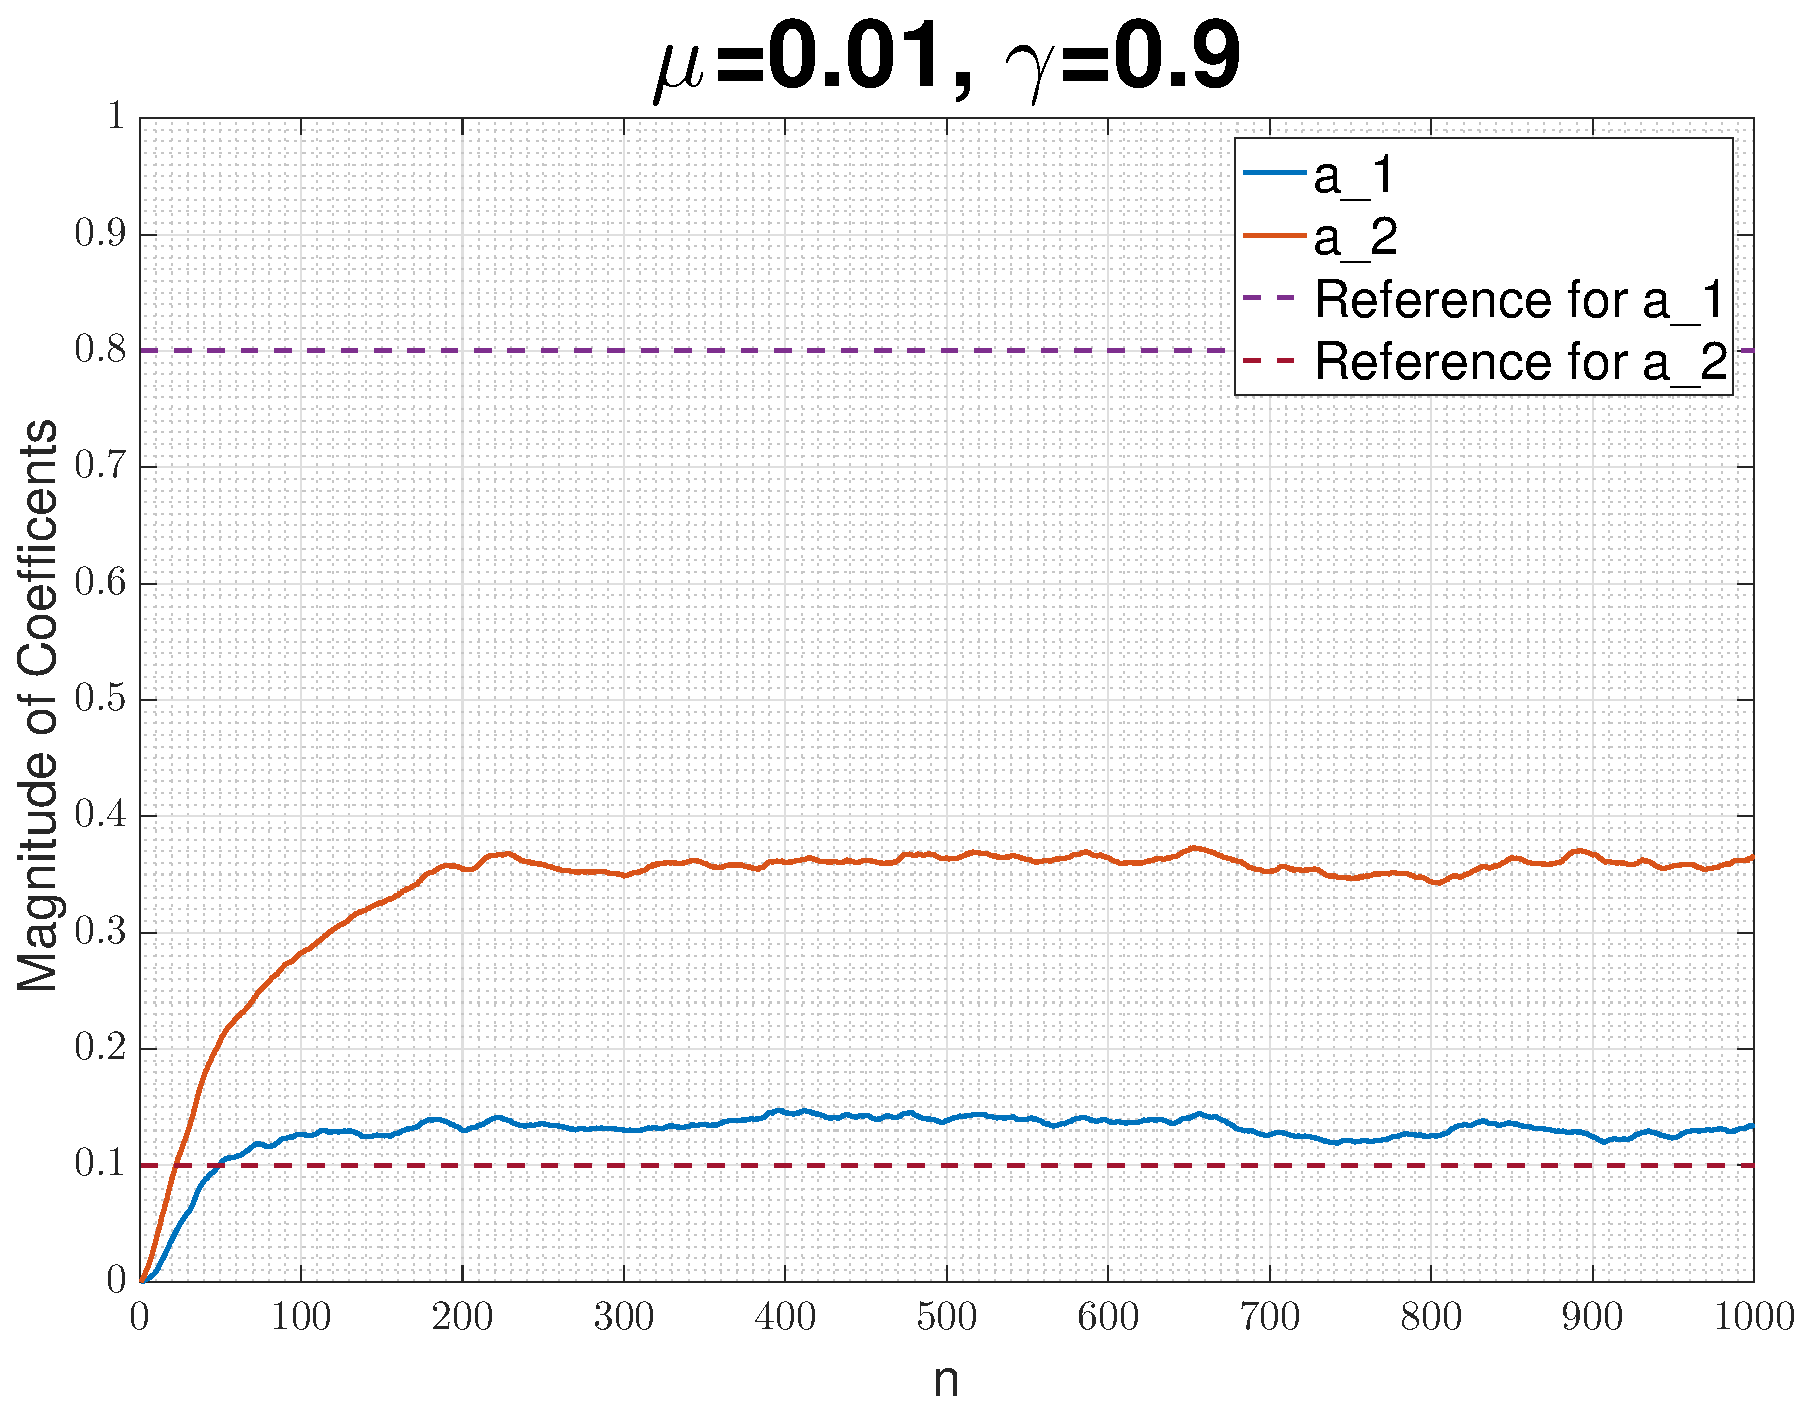
\includegraphics[width=0.32\textwidth]{part3/leaky_mu_01_gamma_09}
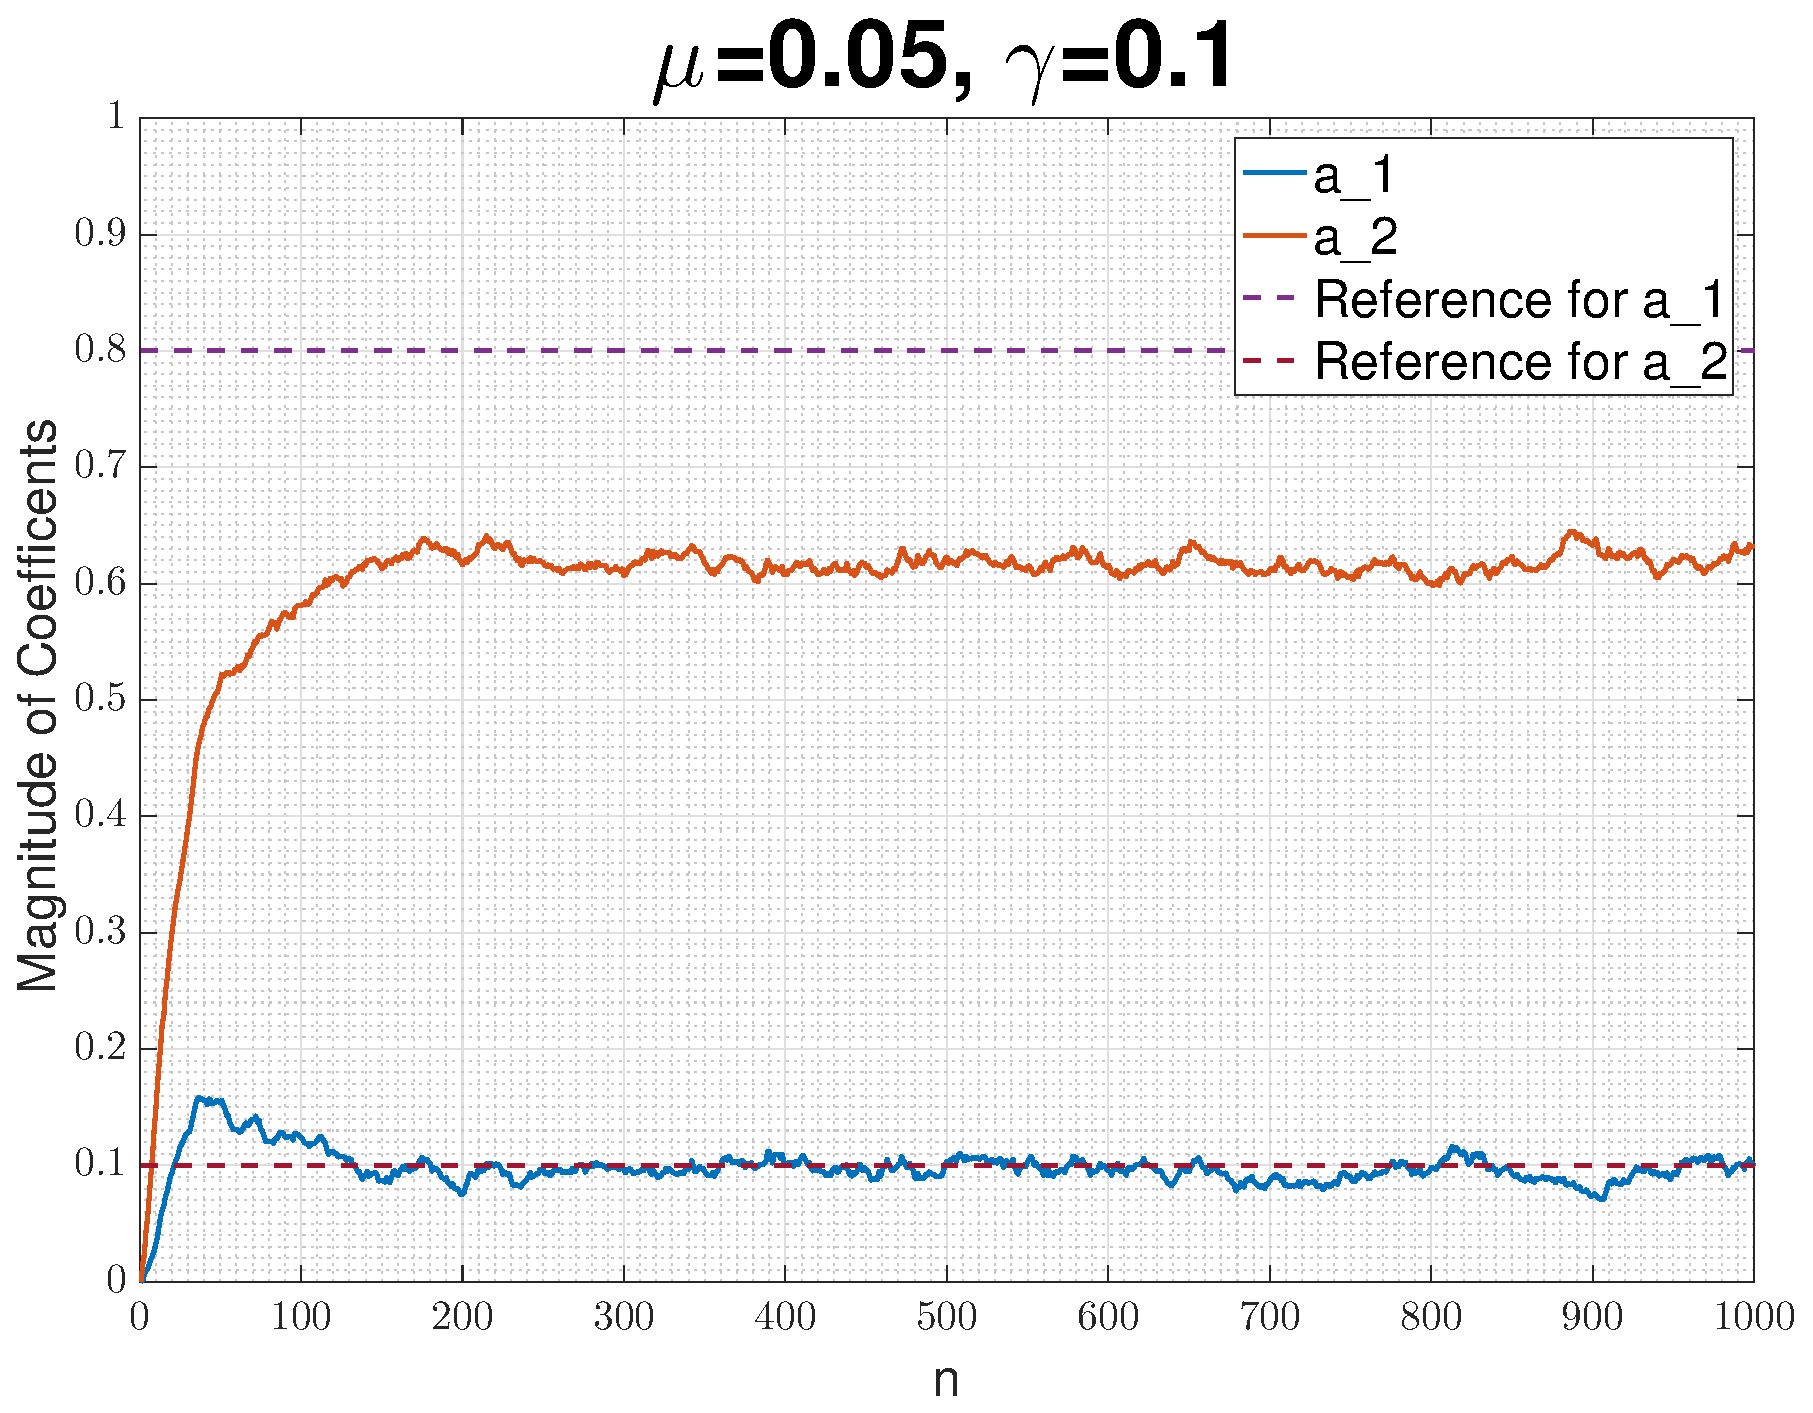
\includegraphics[width=0.32\textwidth]{part3/leaky_mu_05_gamma_01}
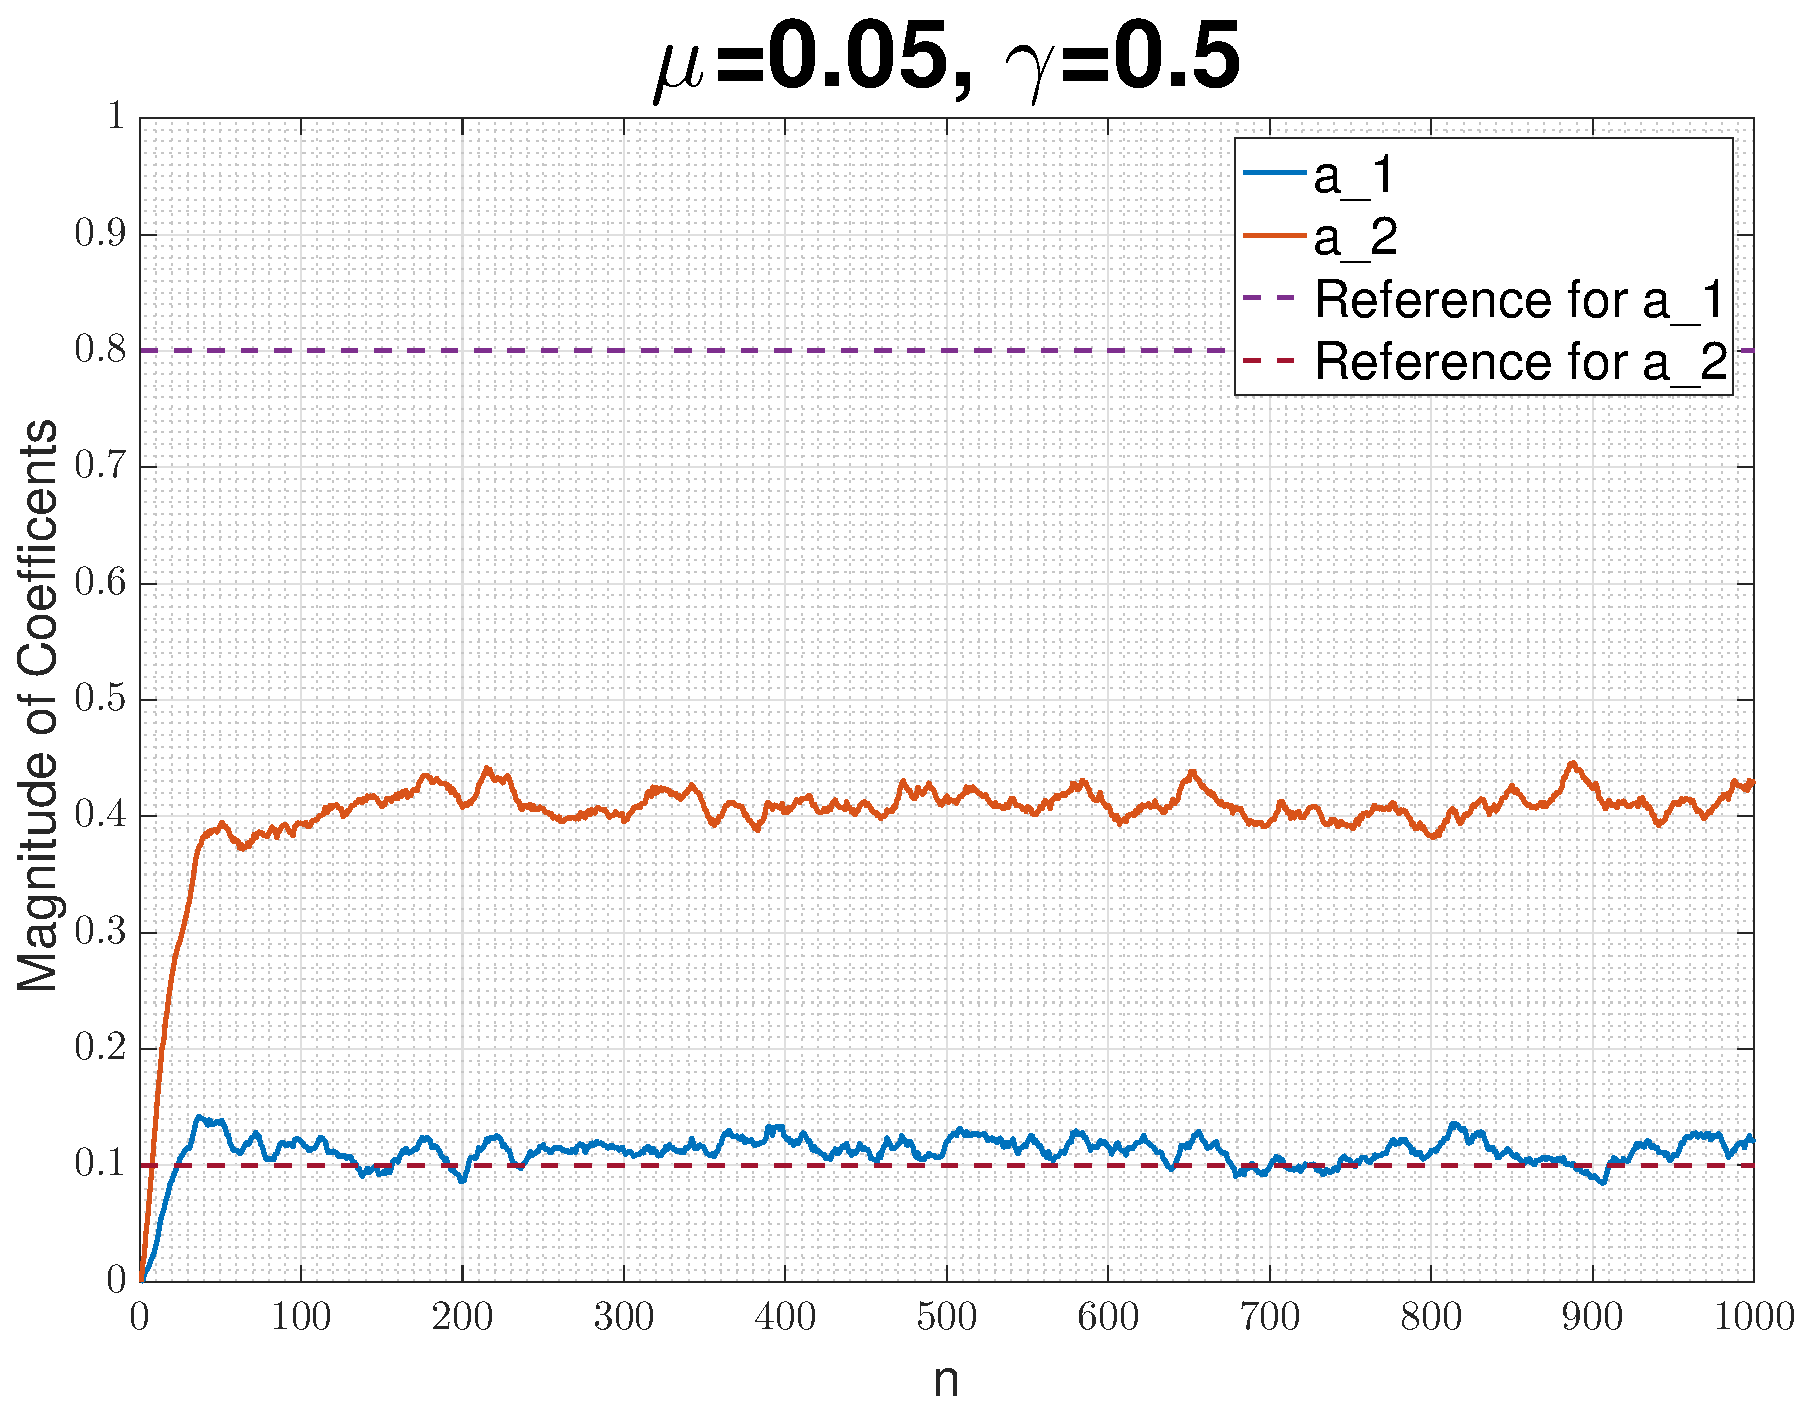
\includegraphics[width=0.32\textwidth]{part3/leaky_mu_05_gamma_05}
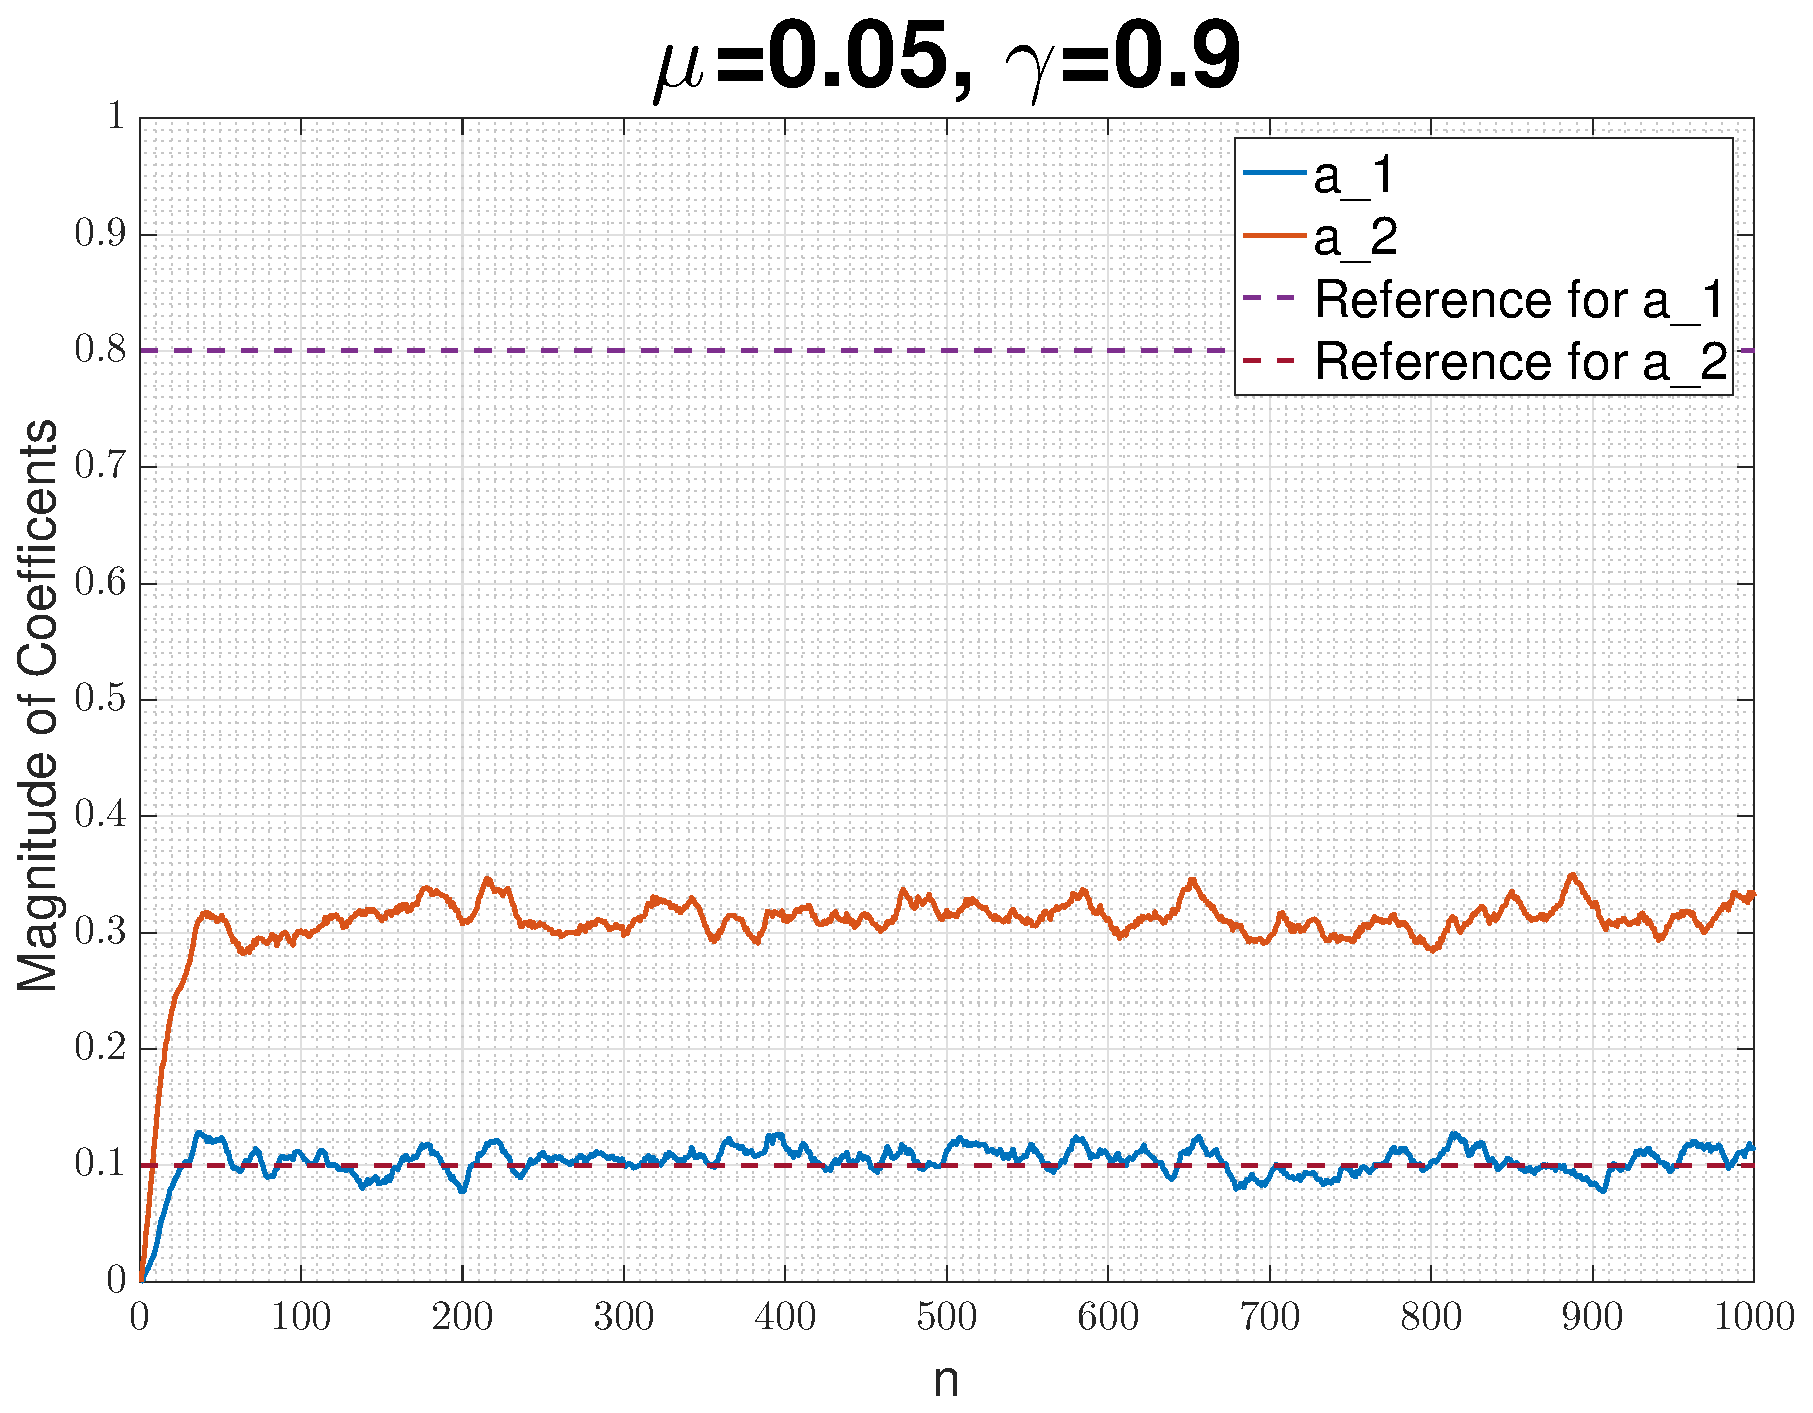
\includegraphics[width=0.32\textwidth]{part3/leaky_mu_05_gamma_09}
\caption{Effect of increasing $\gamma$ on the Steady State Values of Coefficients $a_1$ and $a_2$, for $\mu=0.01$ and $\mu=0.05$}
\label{fig:leaky_lms}
\end{figure}

\subsection{Adaptive Step Sizes}

\noindent{}a. Using the LMS algorithm, we have shown the effect that $\mu$ has on the convergence time as well as the misadjustment. Depending on the application, we can vary $\mu$ to satisfy constraints on convergence time or overshoot or steady-state error. The non-varying nature of $\mu$ makes the LMS algorithm computationally cheap. However, the flexibility the choice of $\mu$ has certain shortcomings, a major one being that certain choices if $\mu$ can cause the algorithm to diverge instead of converging. \\

\noindent{}The Gradient Adaptive Step Size (GASS) algorithms allow $\mu$ to be time-varying. The algorithms are generally implemented such that the steady-state learning rates approach 0, thereby ensuring stability and convergence. 

\begin{figure}[H]
\centering{}
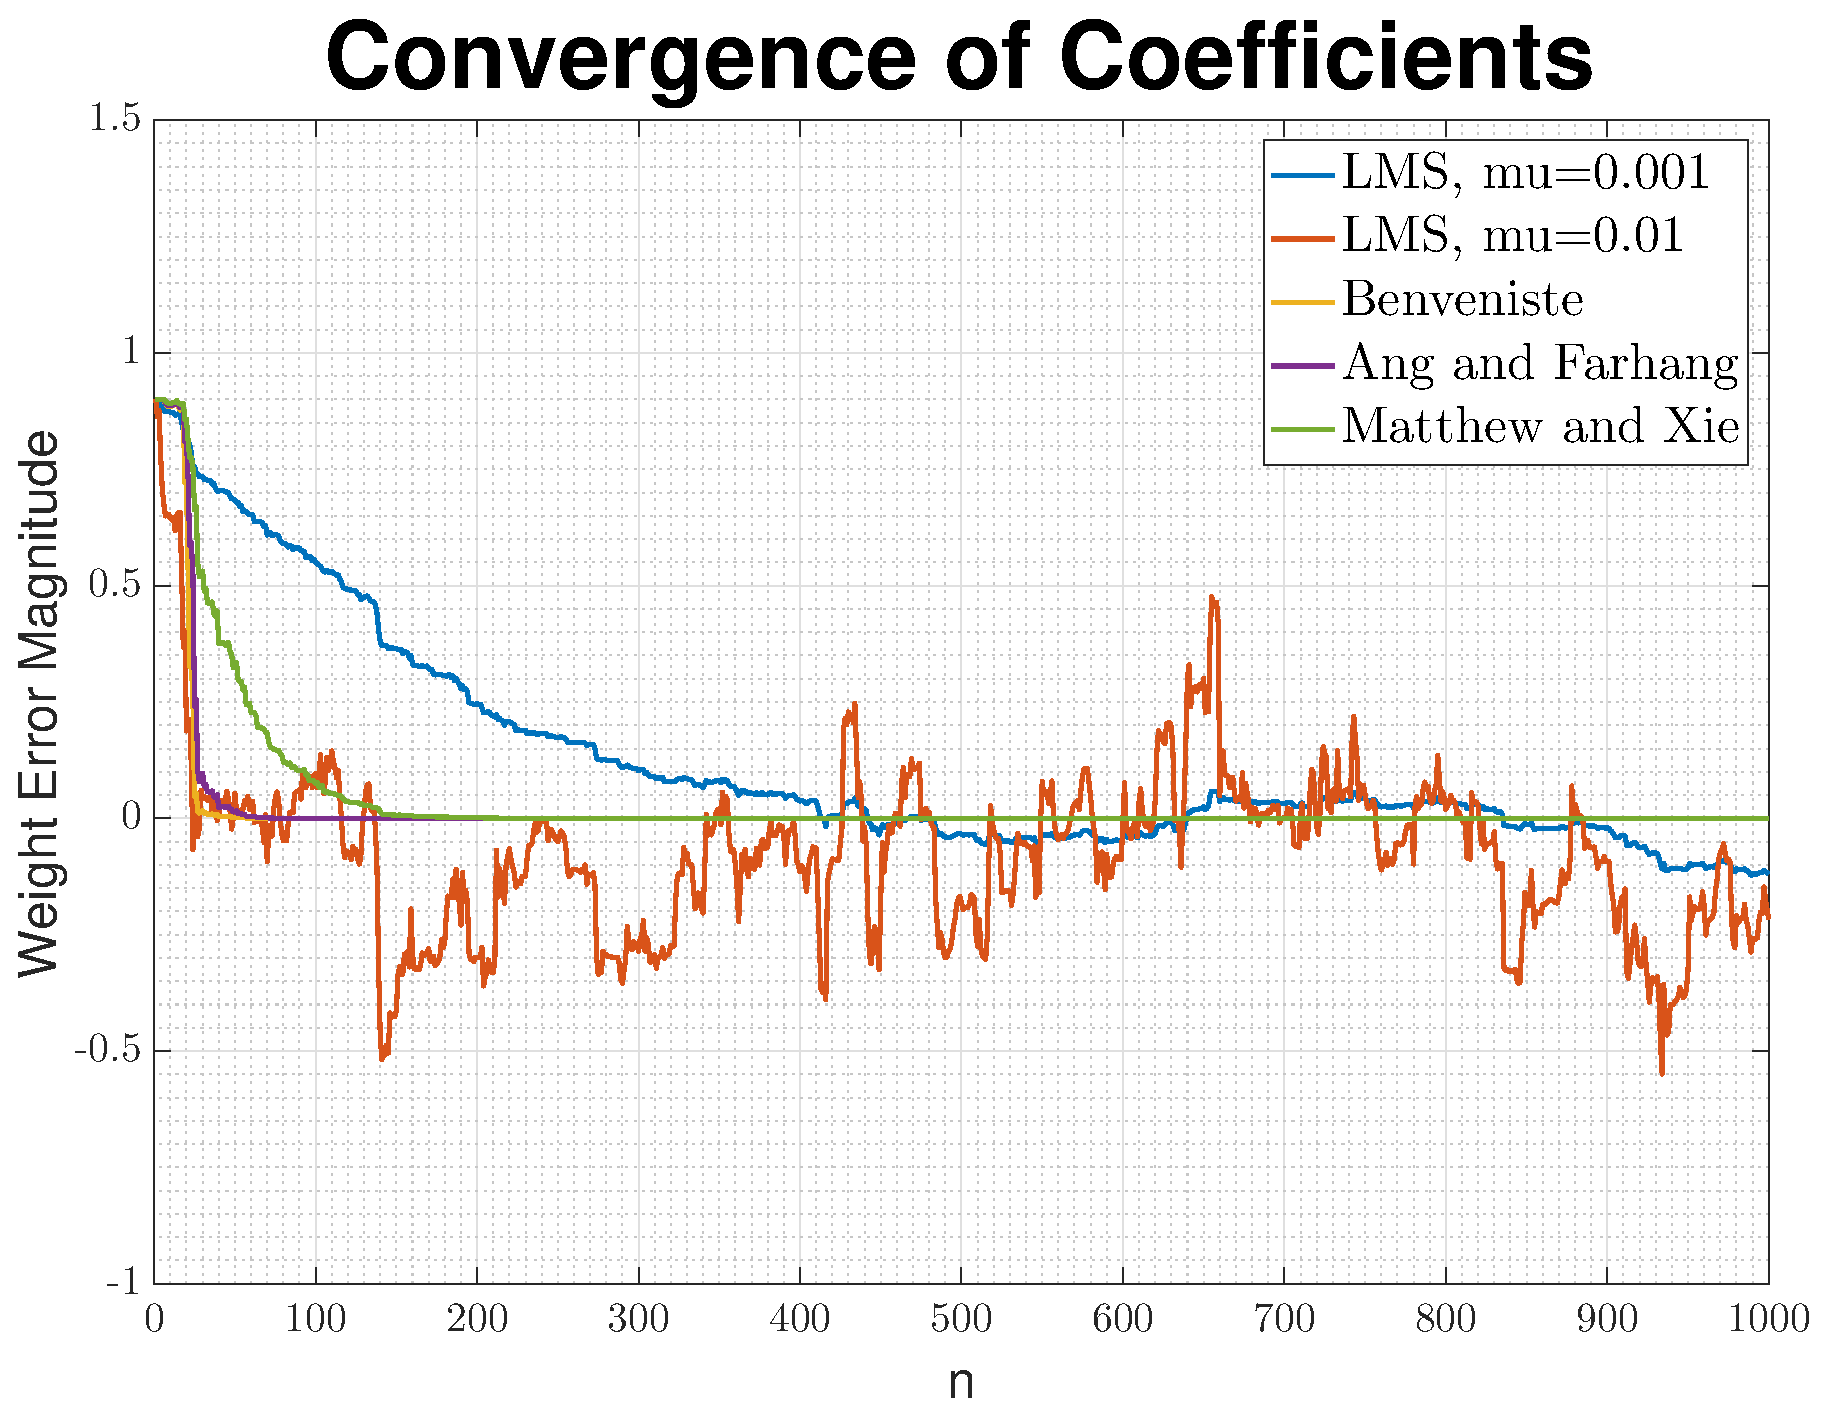
\includegraphics[width=0.32\textwidth]{part3/convergence_of_weights}
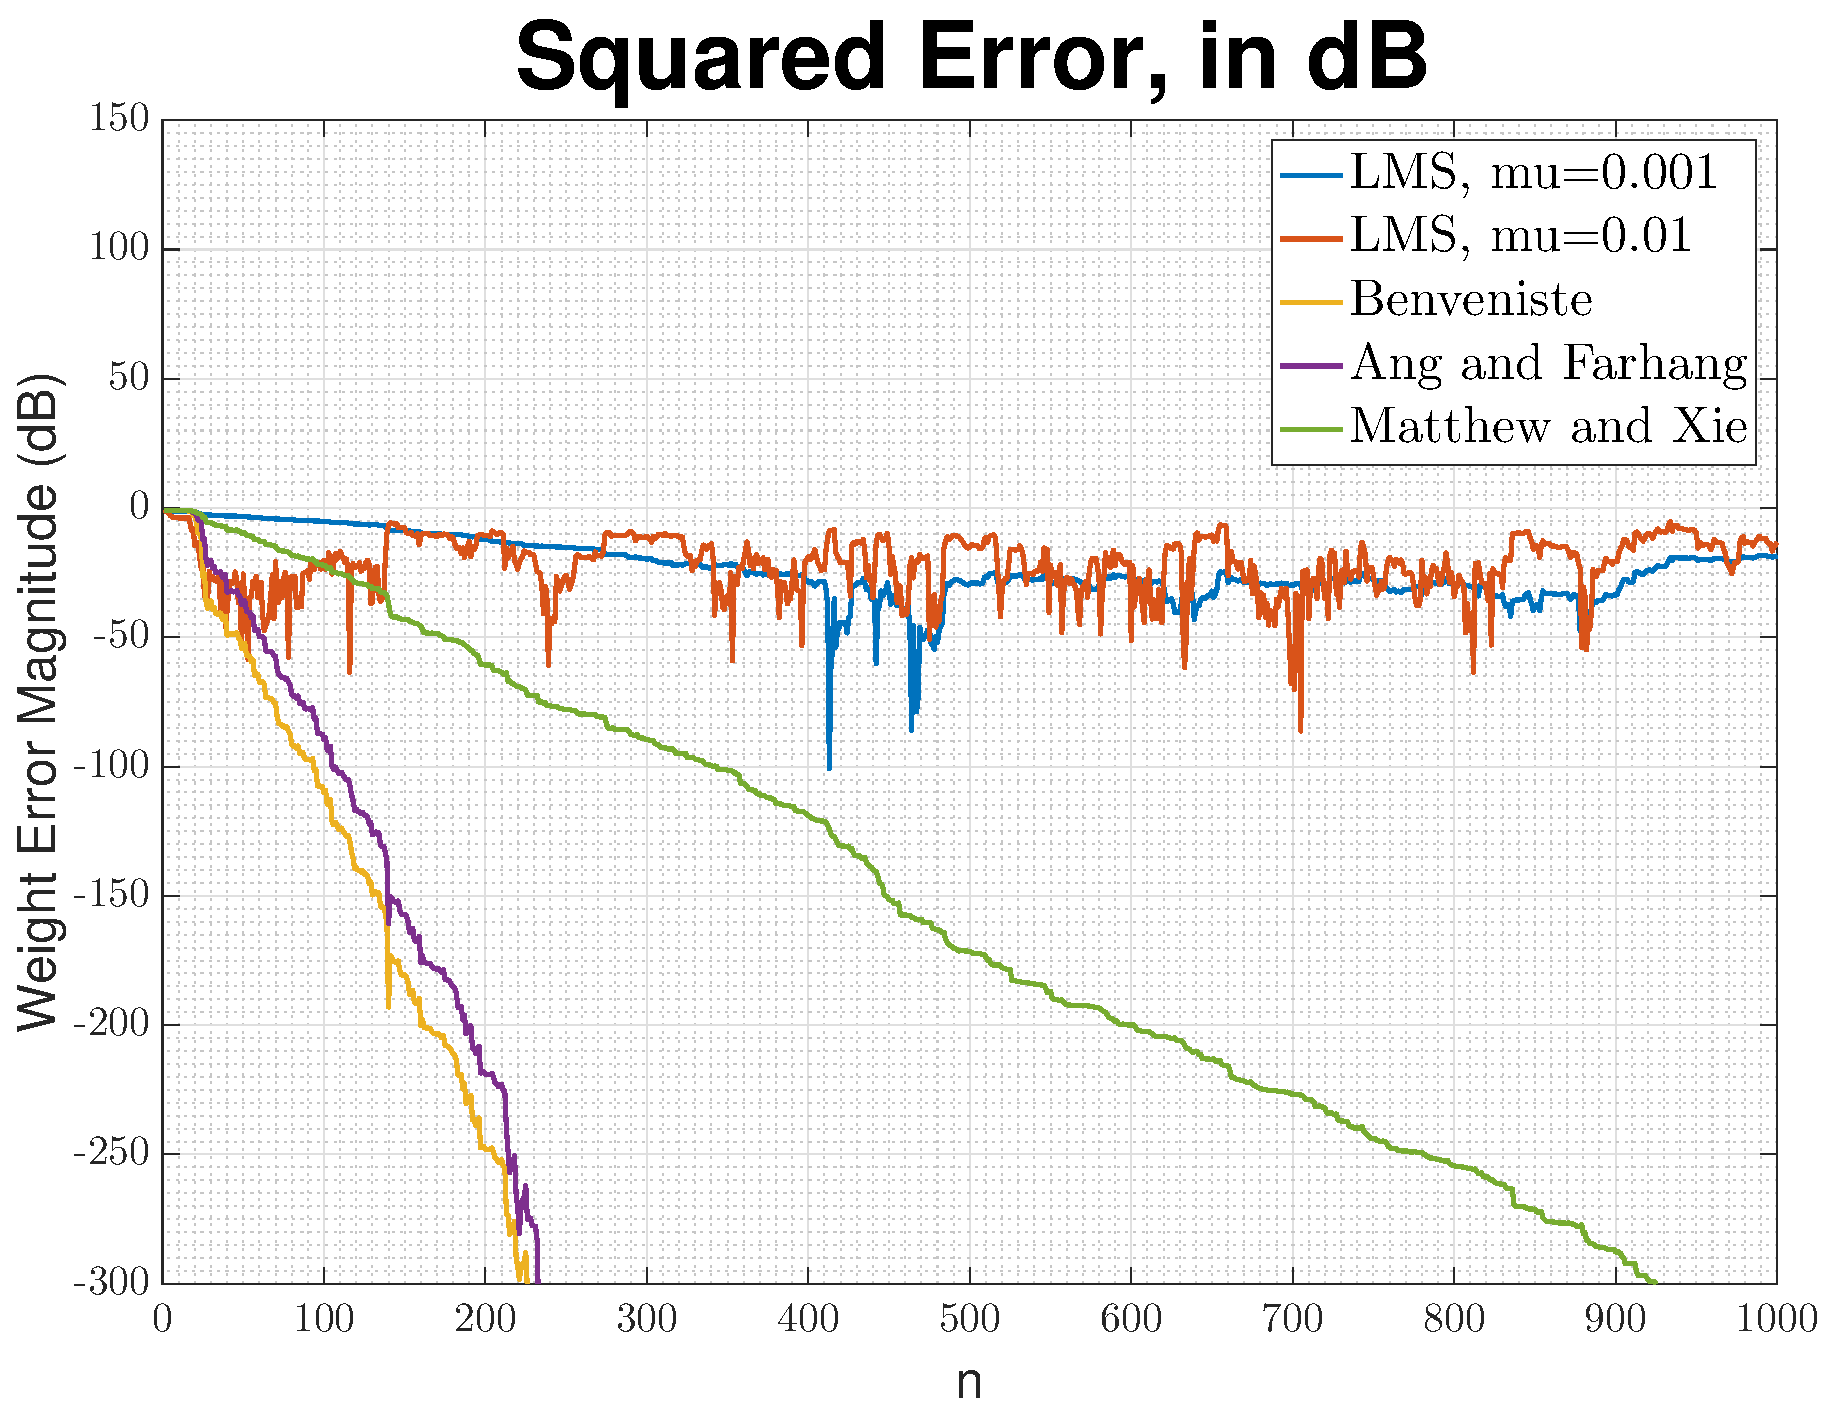
\includegraphics[width=0.32\textwidth]{part3/convergence_of_weights_db}
\caption{Comparison of Convergence Time using Adaptive Step Sizes and Standard LMS Algorithms}
\end{figure}


\begin{figure}[H]
\centering{}
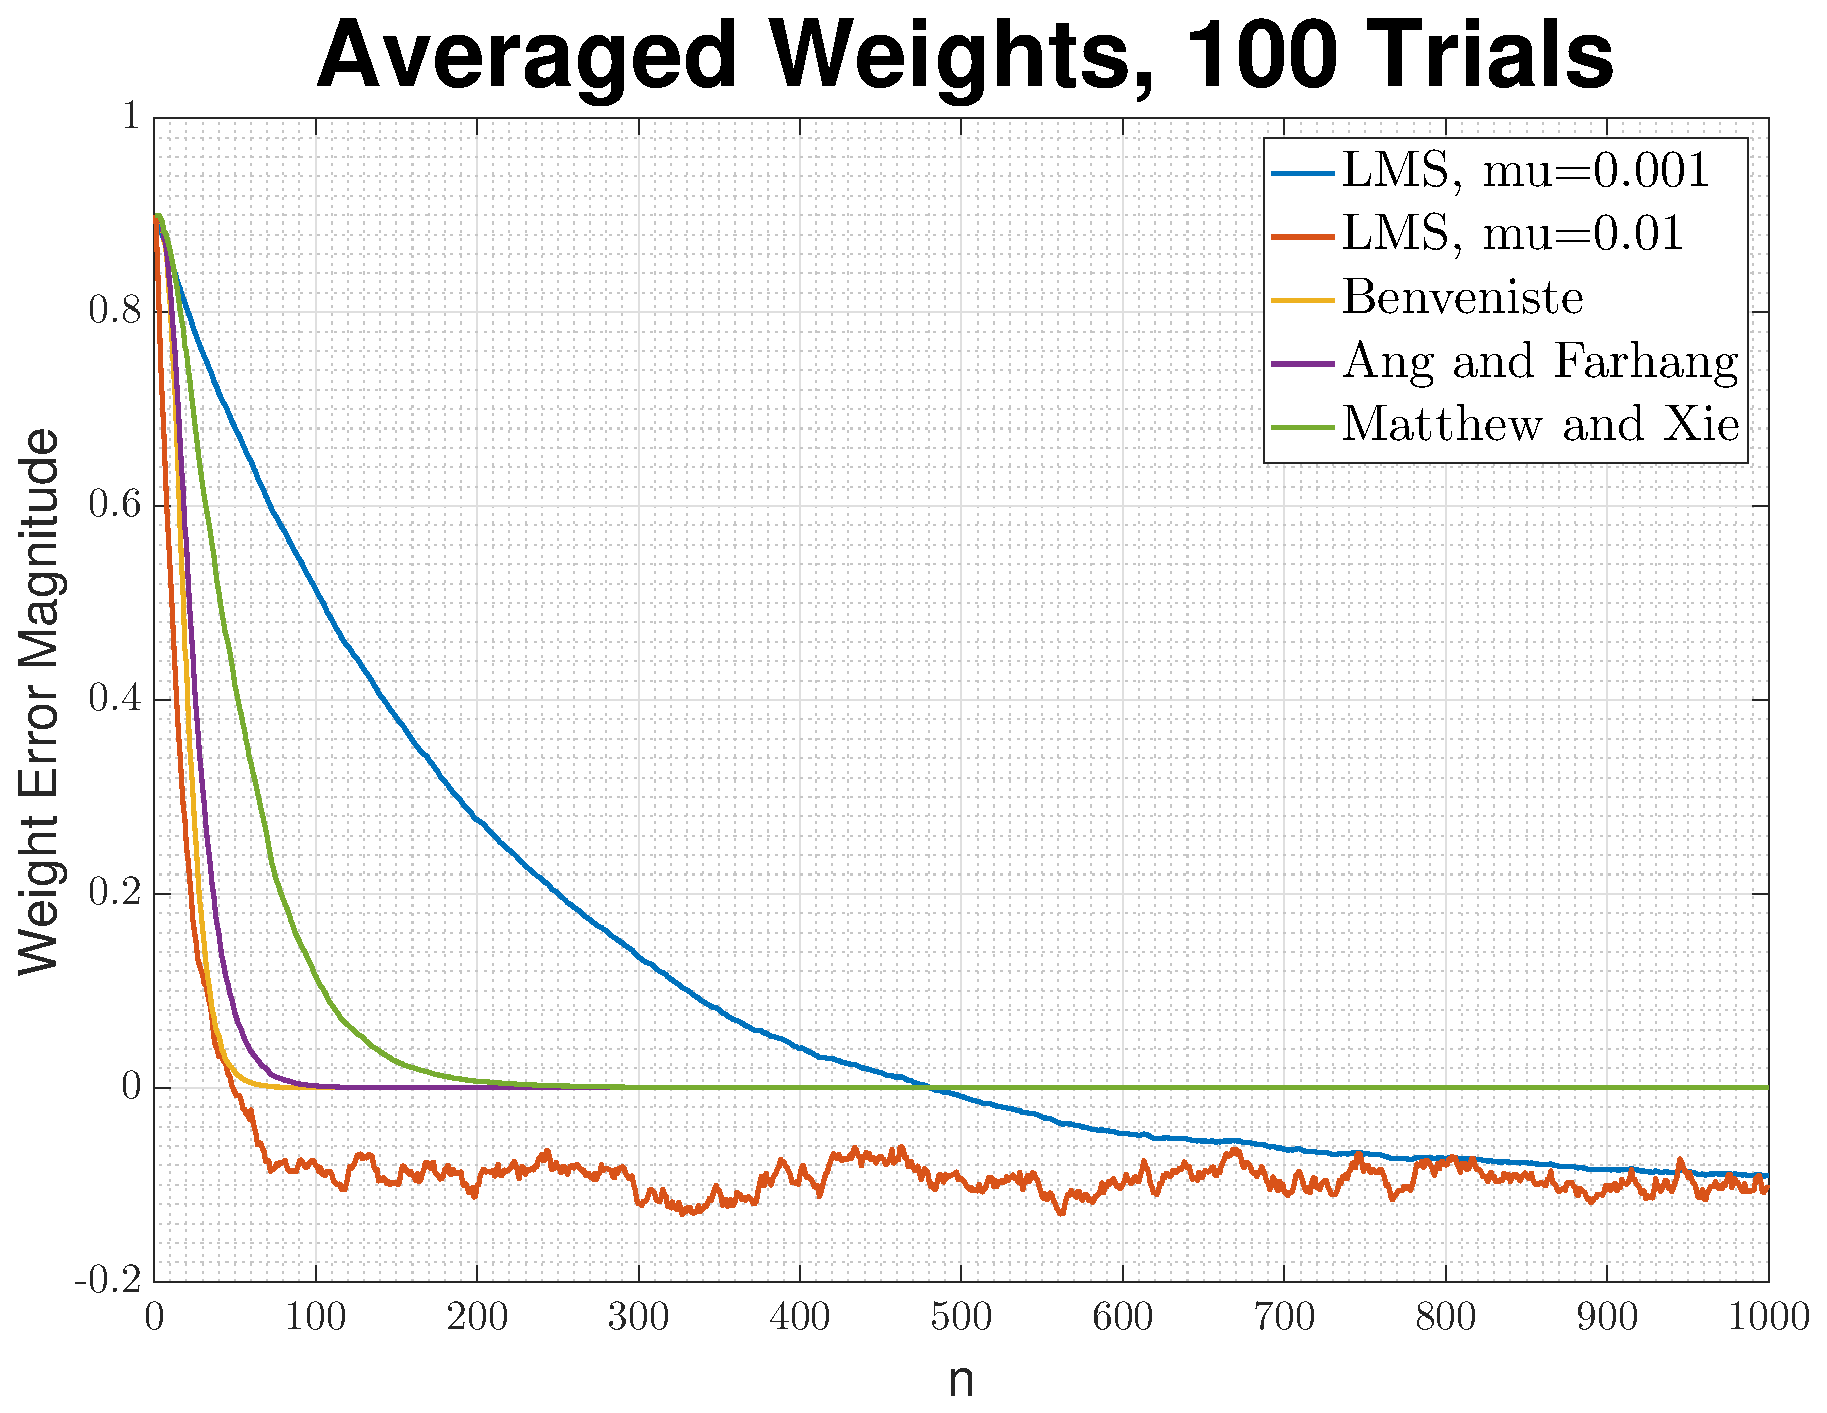
\includegraphics[width=0.32\textwidth]{part3/convergence_of_weights_averaged}
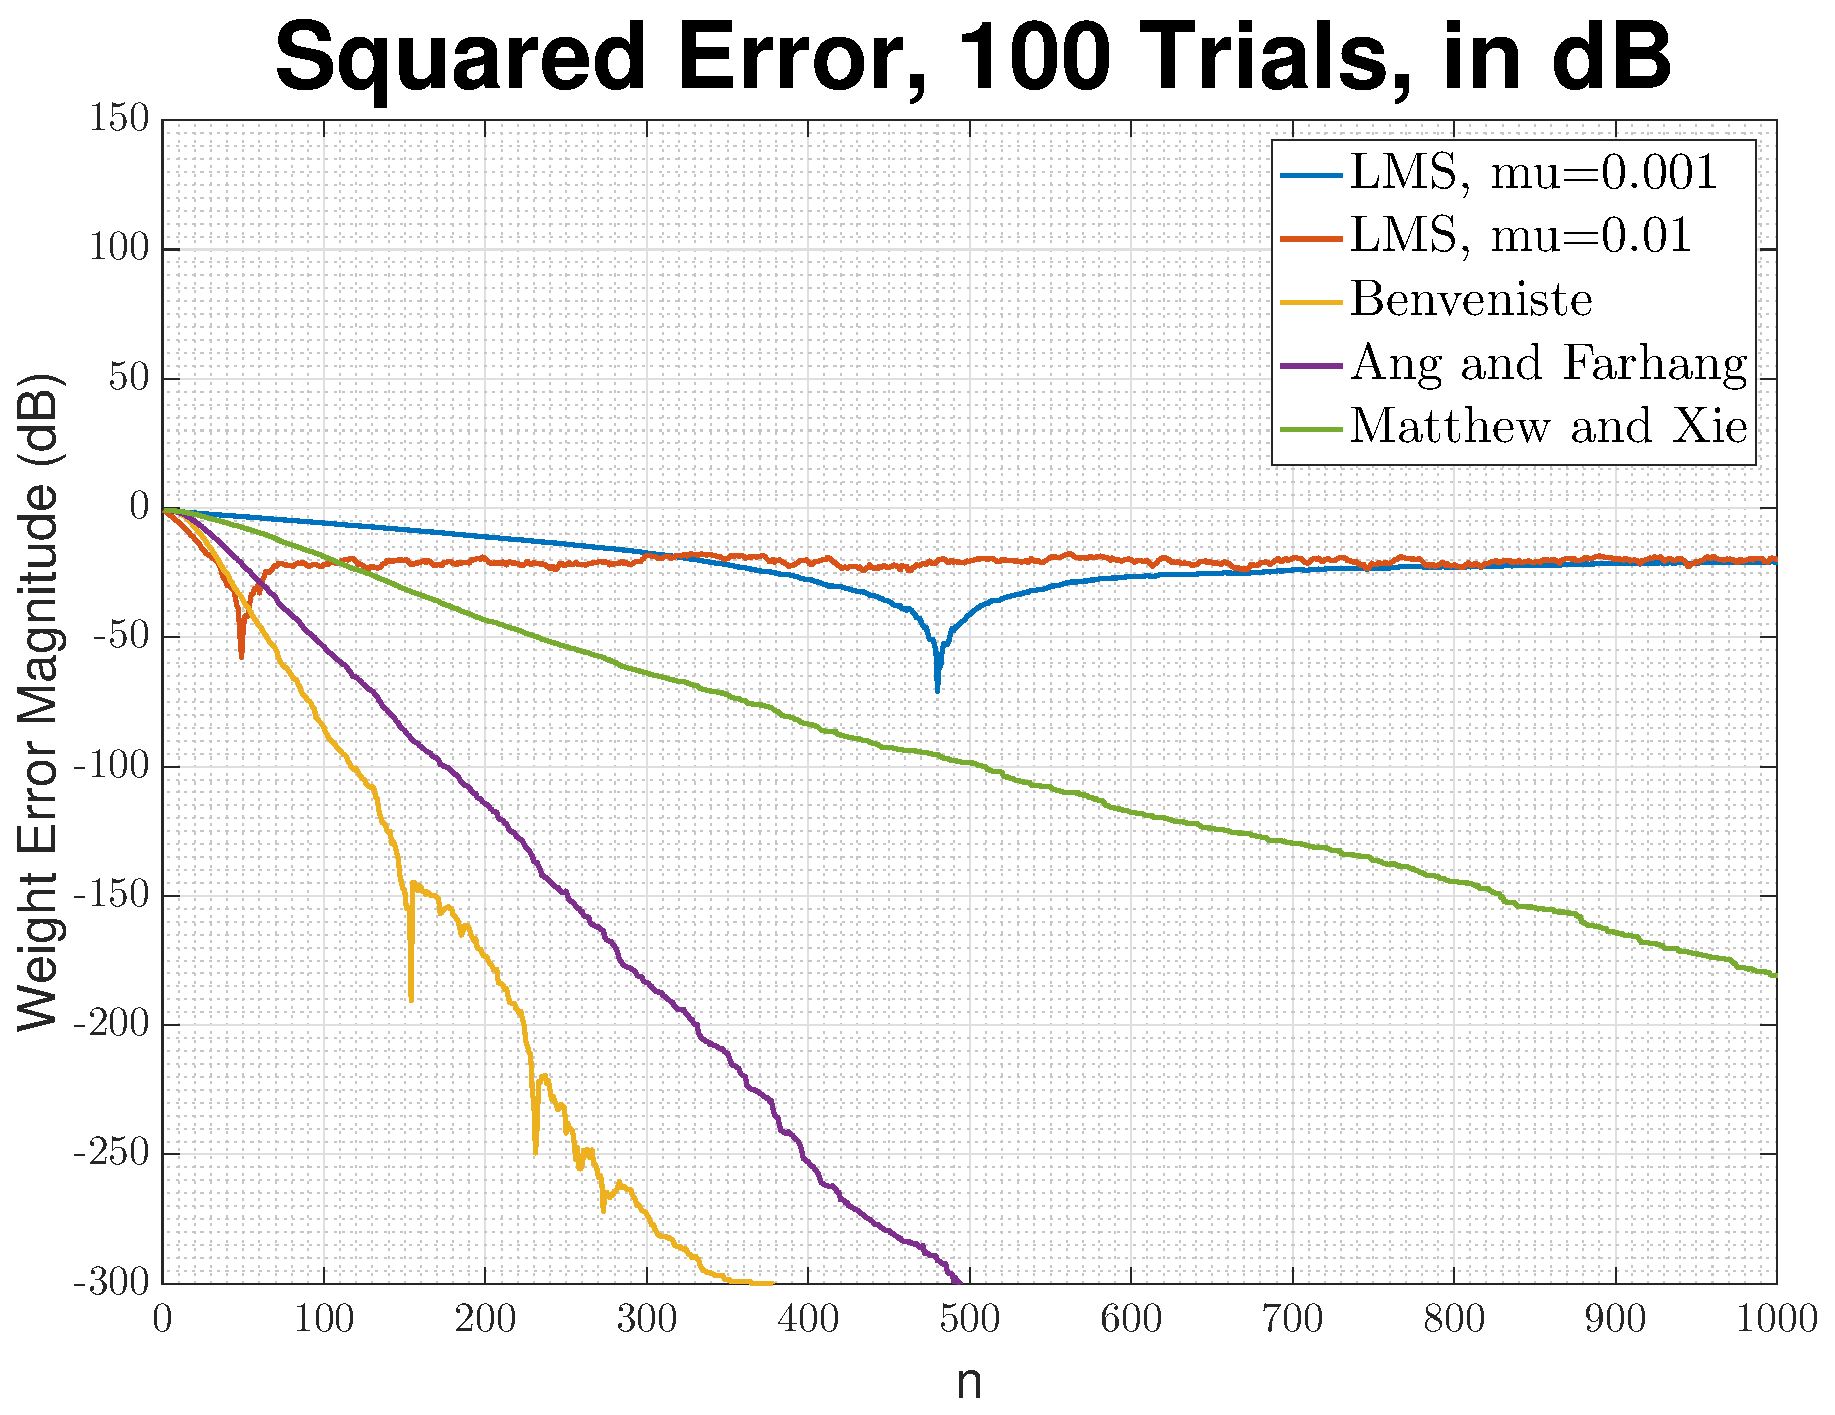
\includegraphics[width=0.32\textwidth]{part3/convergence_of_weights_averaged_db}
\caption{Studying Convergence Time by Averaging Weights over 100 Random Realisations}
\end{figure}


\begin{figure}[H]
\centering{}
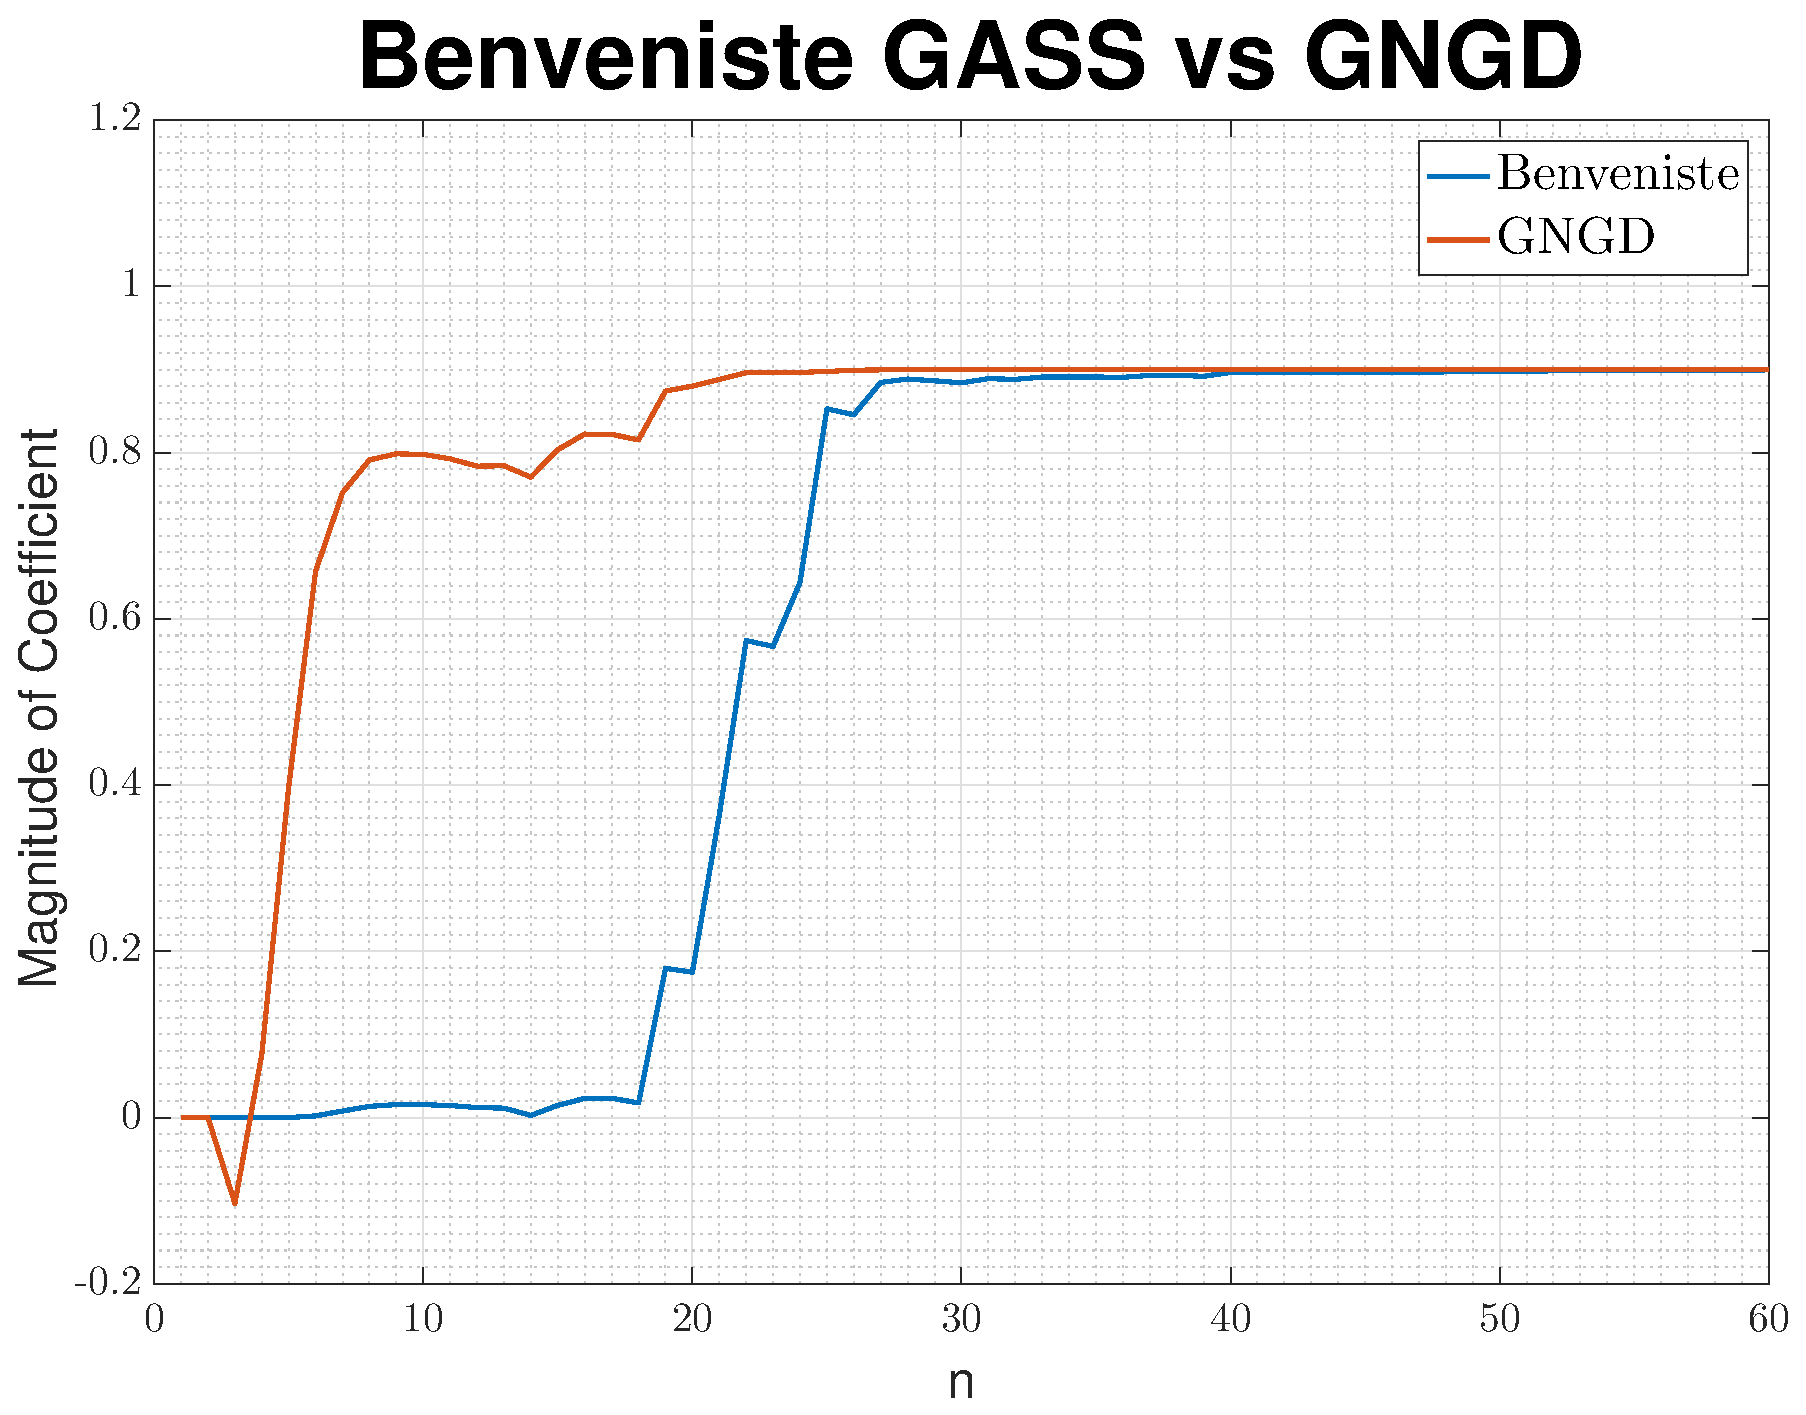
\includegraphics[width=0.32\textwidth]{part3/compare_benveniste_gngd}
\caption{Comparing Convergence Speed of GNGD and Benveniste's GASS Algorithms}
\end{figure}


\begin{figure}[H]
\centering{}
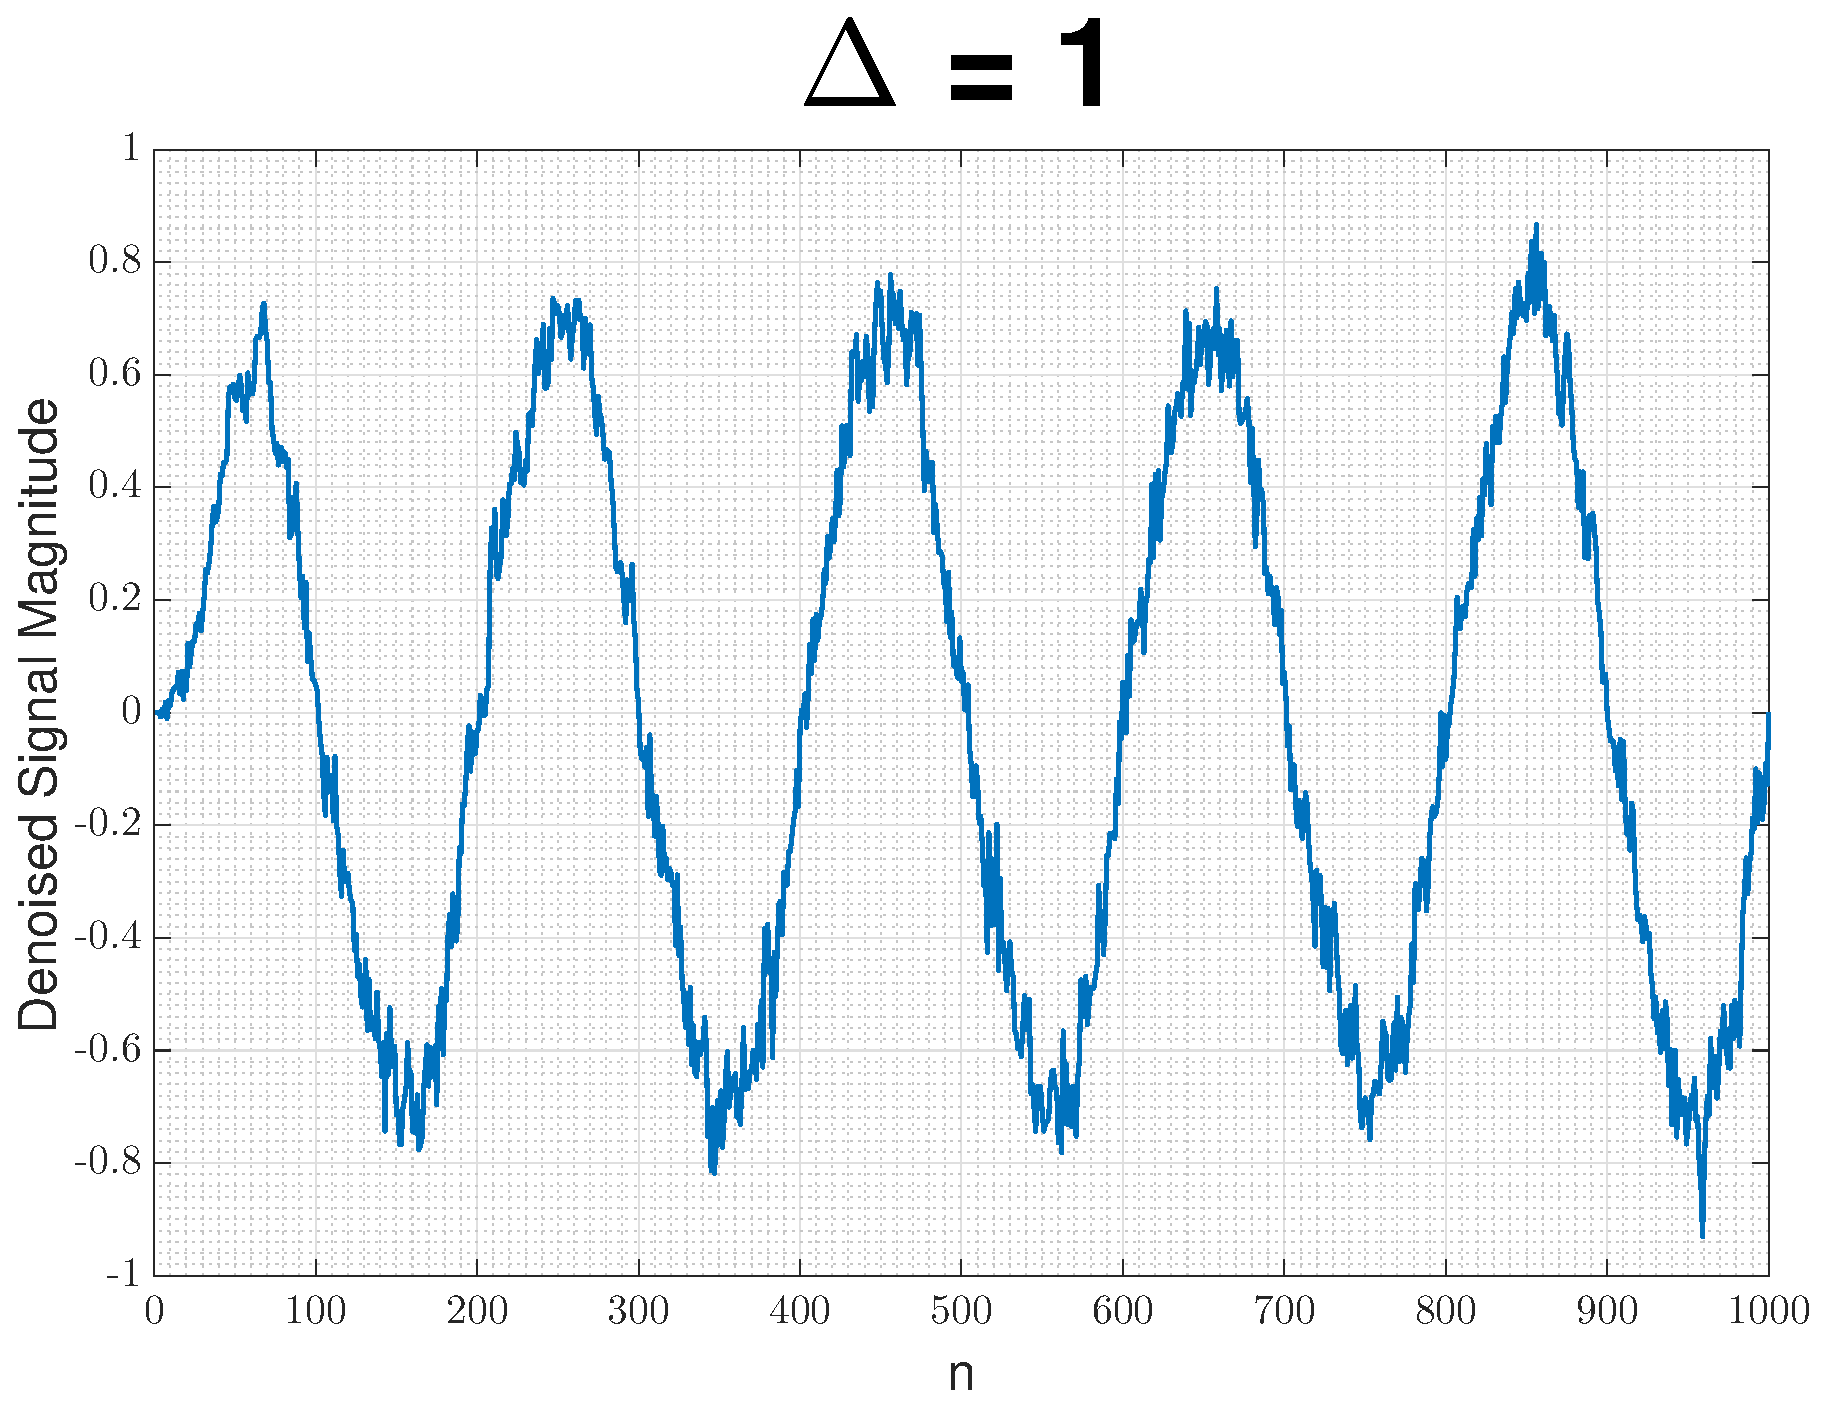
\includegraphics[width=0.24\textwidth]{part3/delay_1}
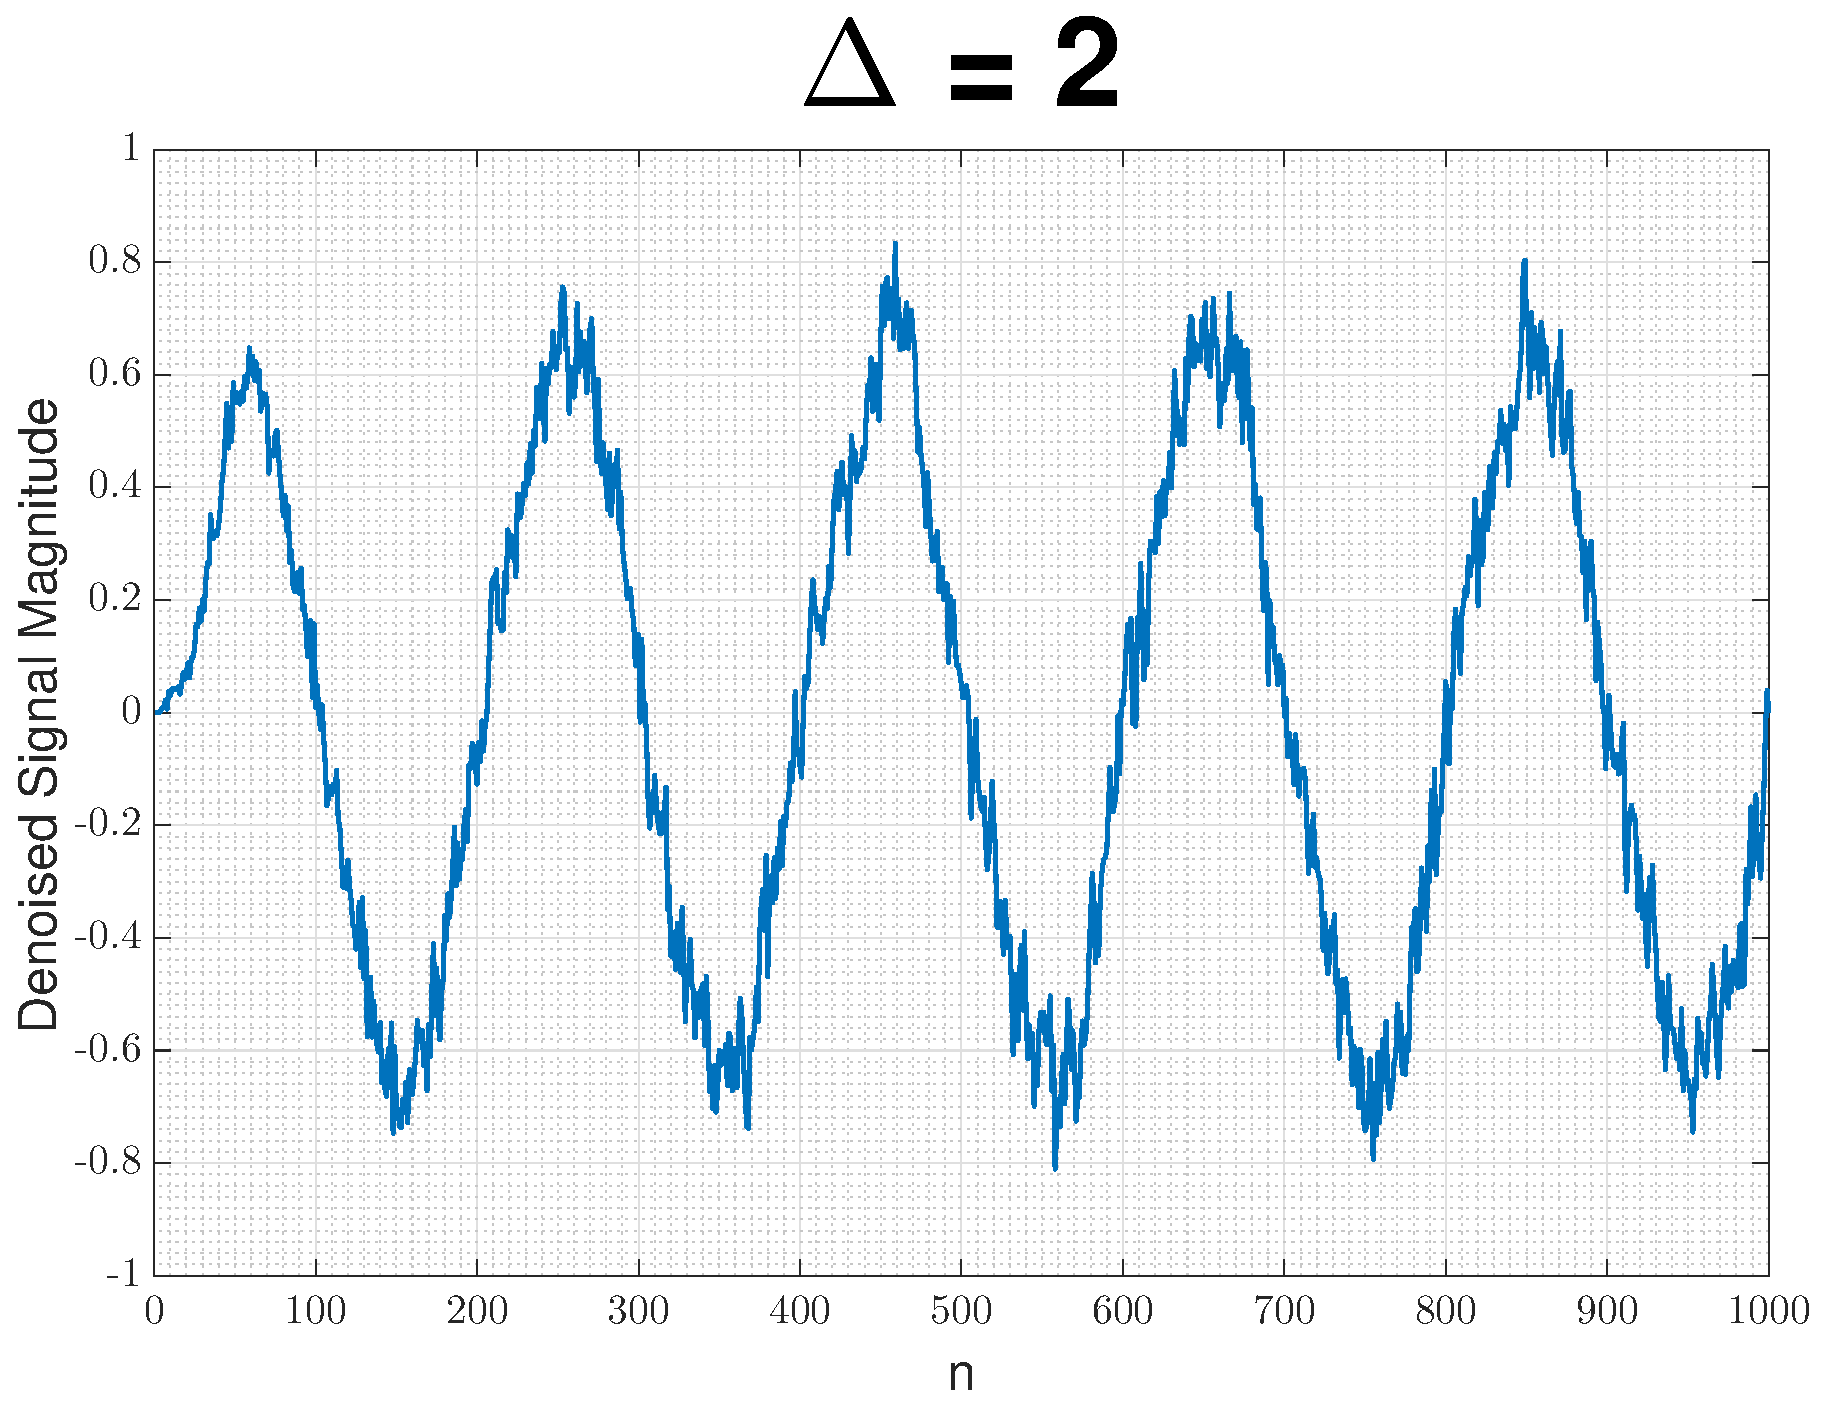
\includegraphics[width=0.24\textwidth]{part3/delay_2}
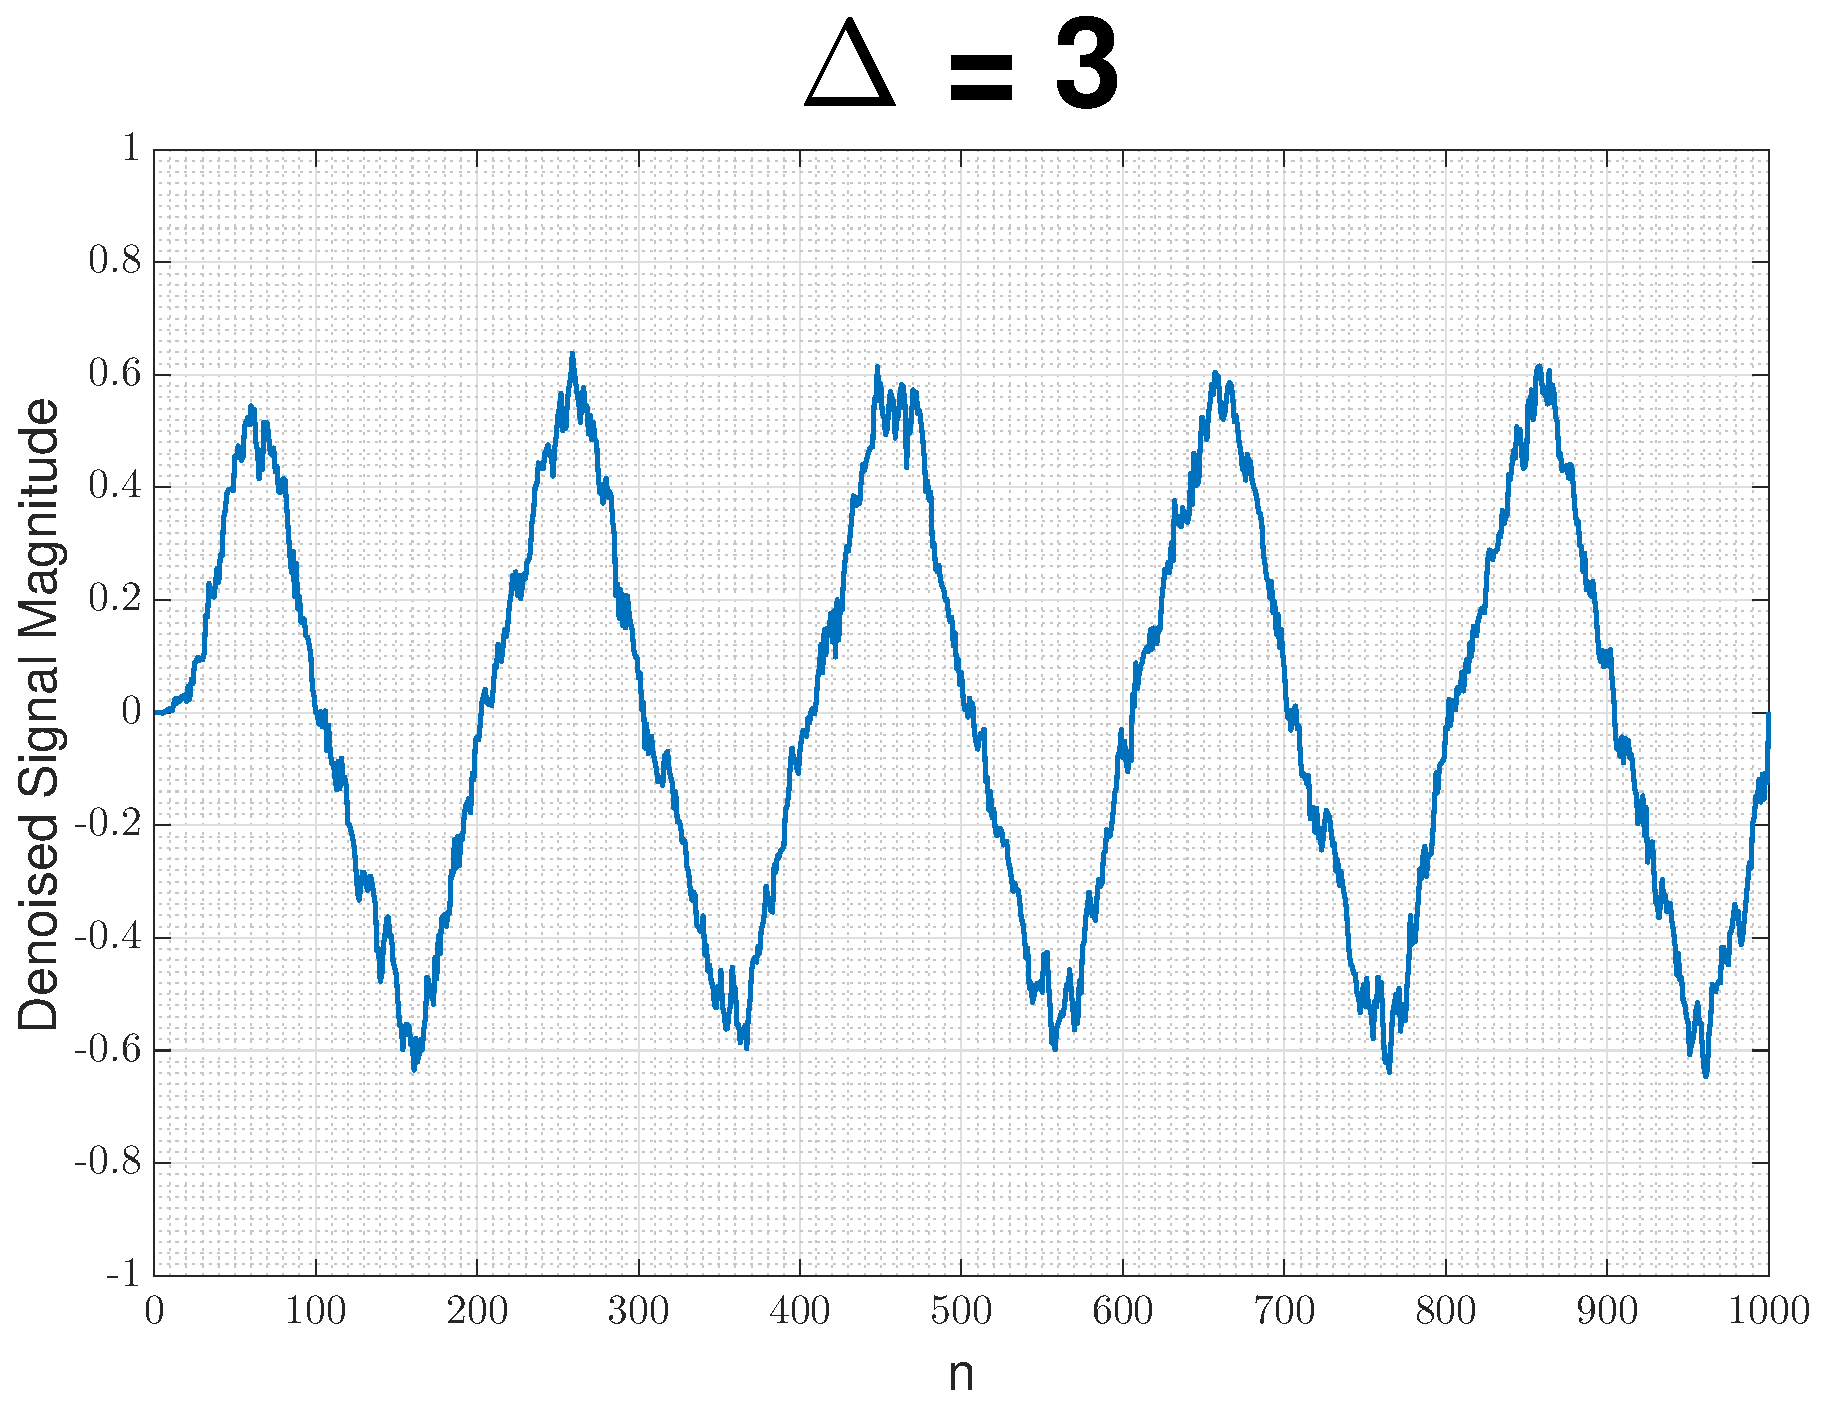
\includegraphics[width=0.24\textwidth]{part3/delay_3}
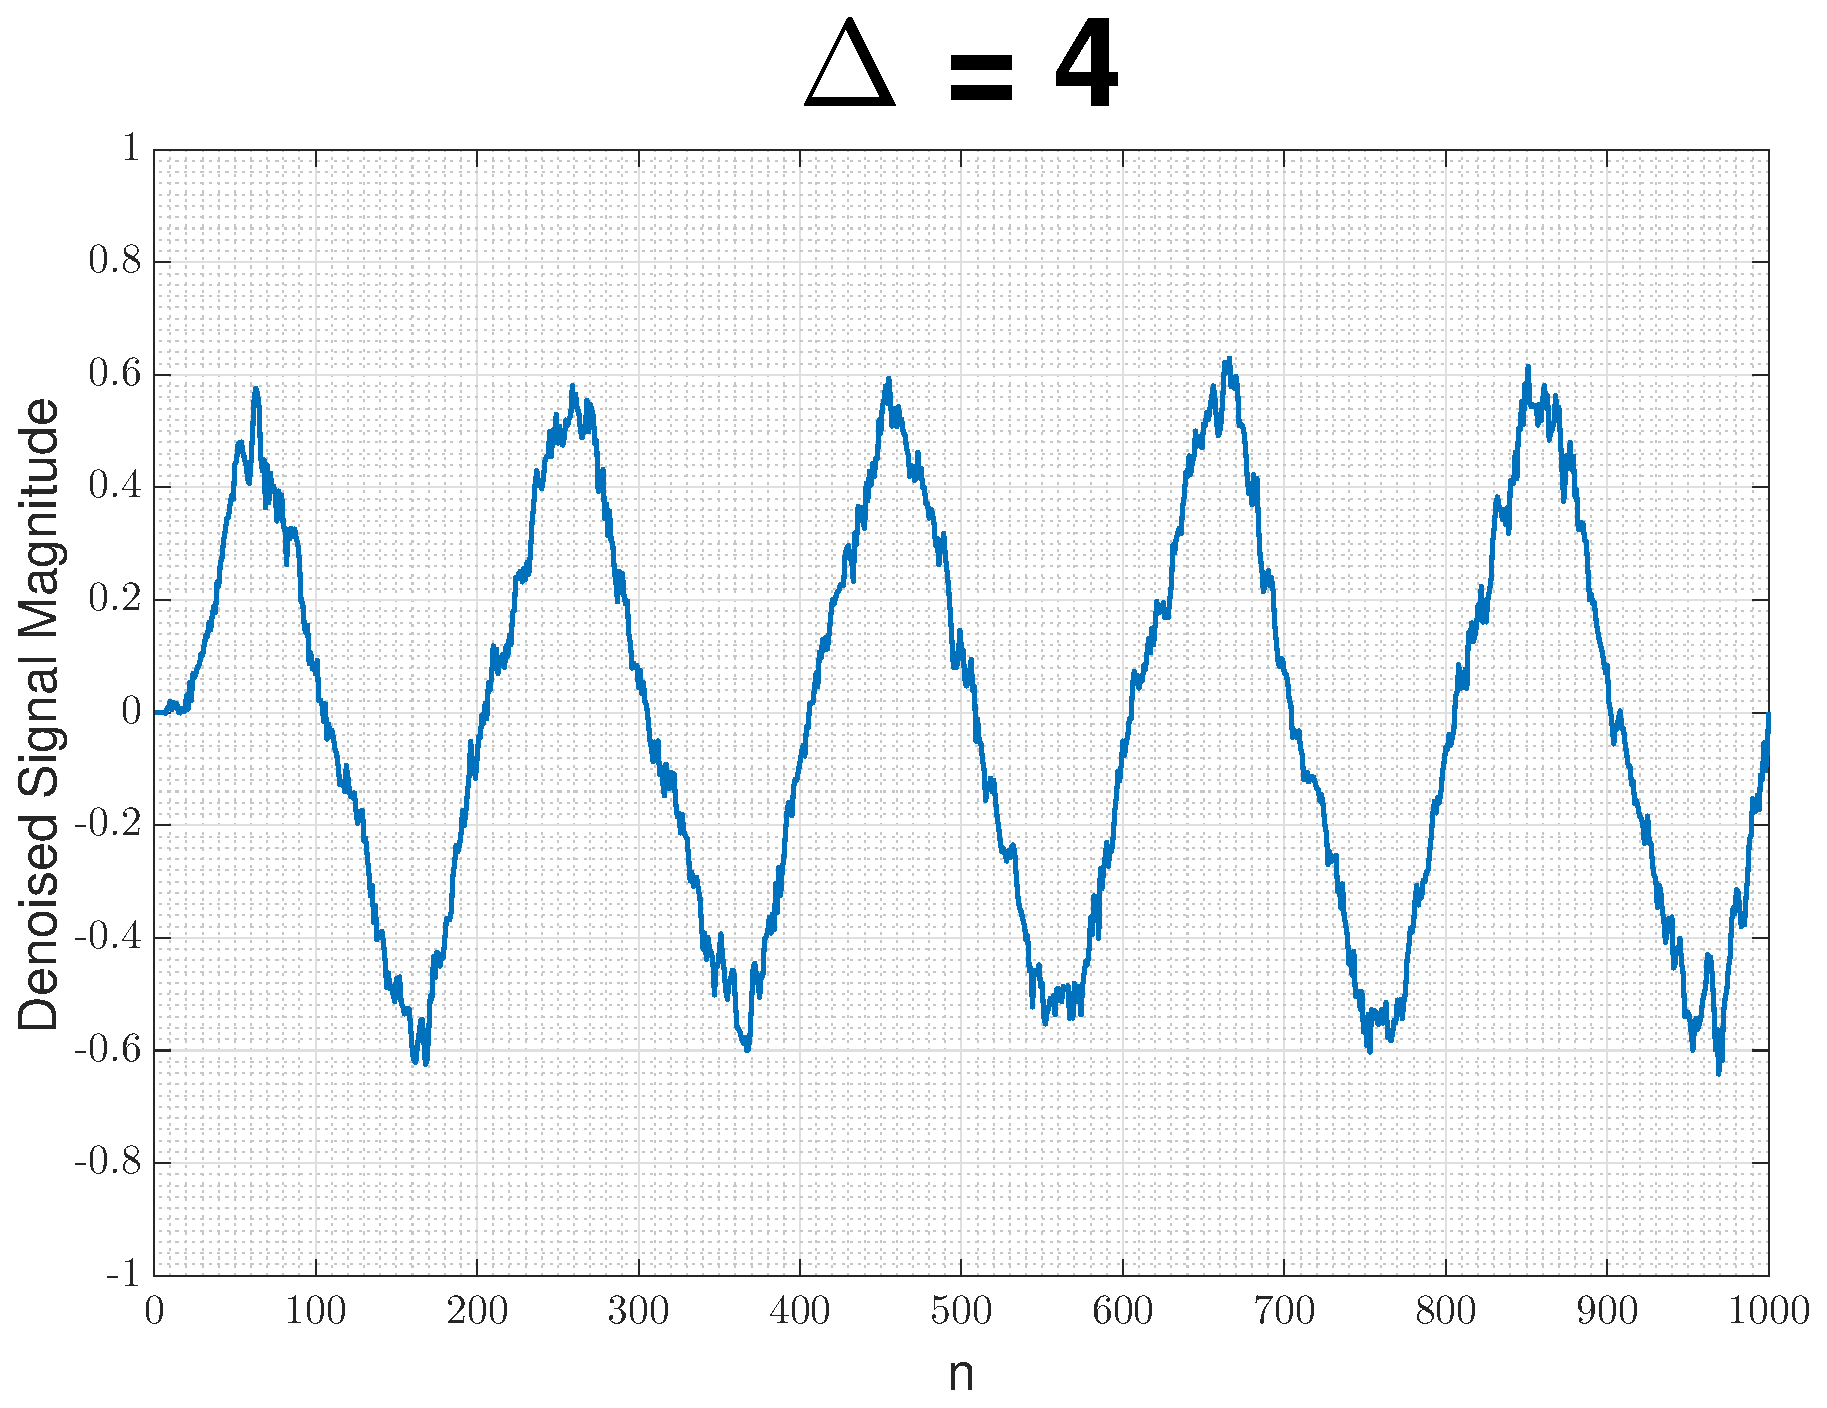
\includegraphics[width=0.24\textwidth]{part3/delay_4}
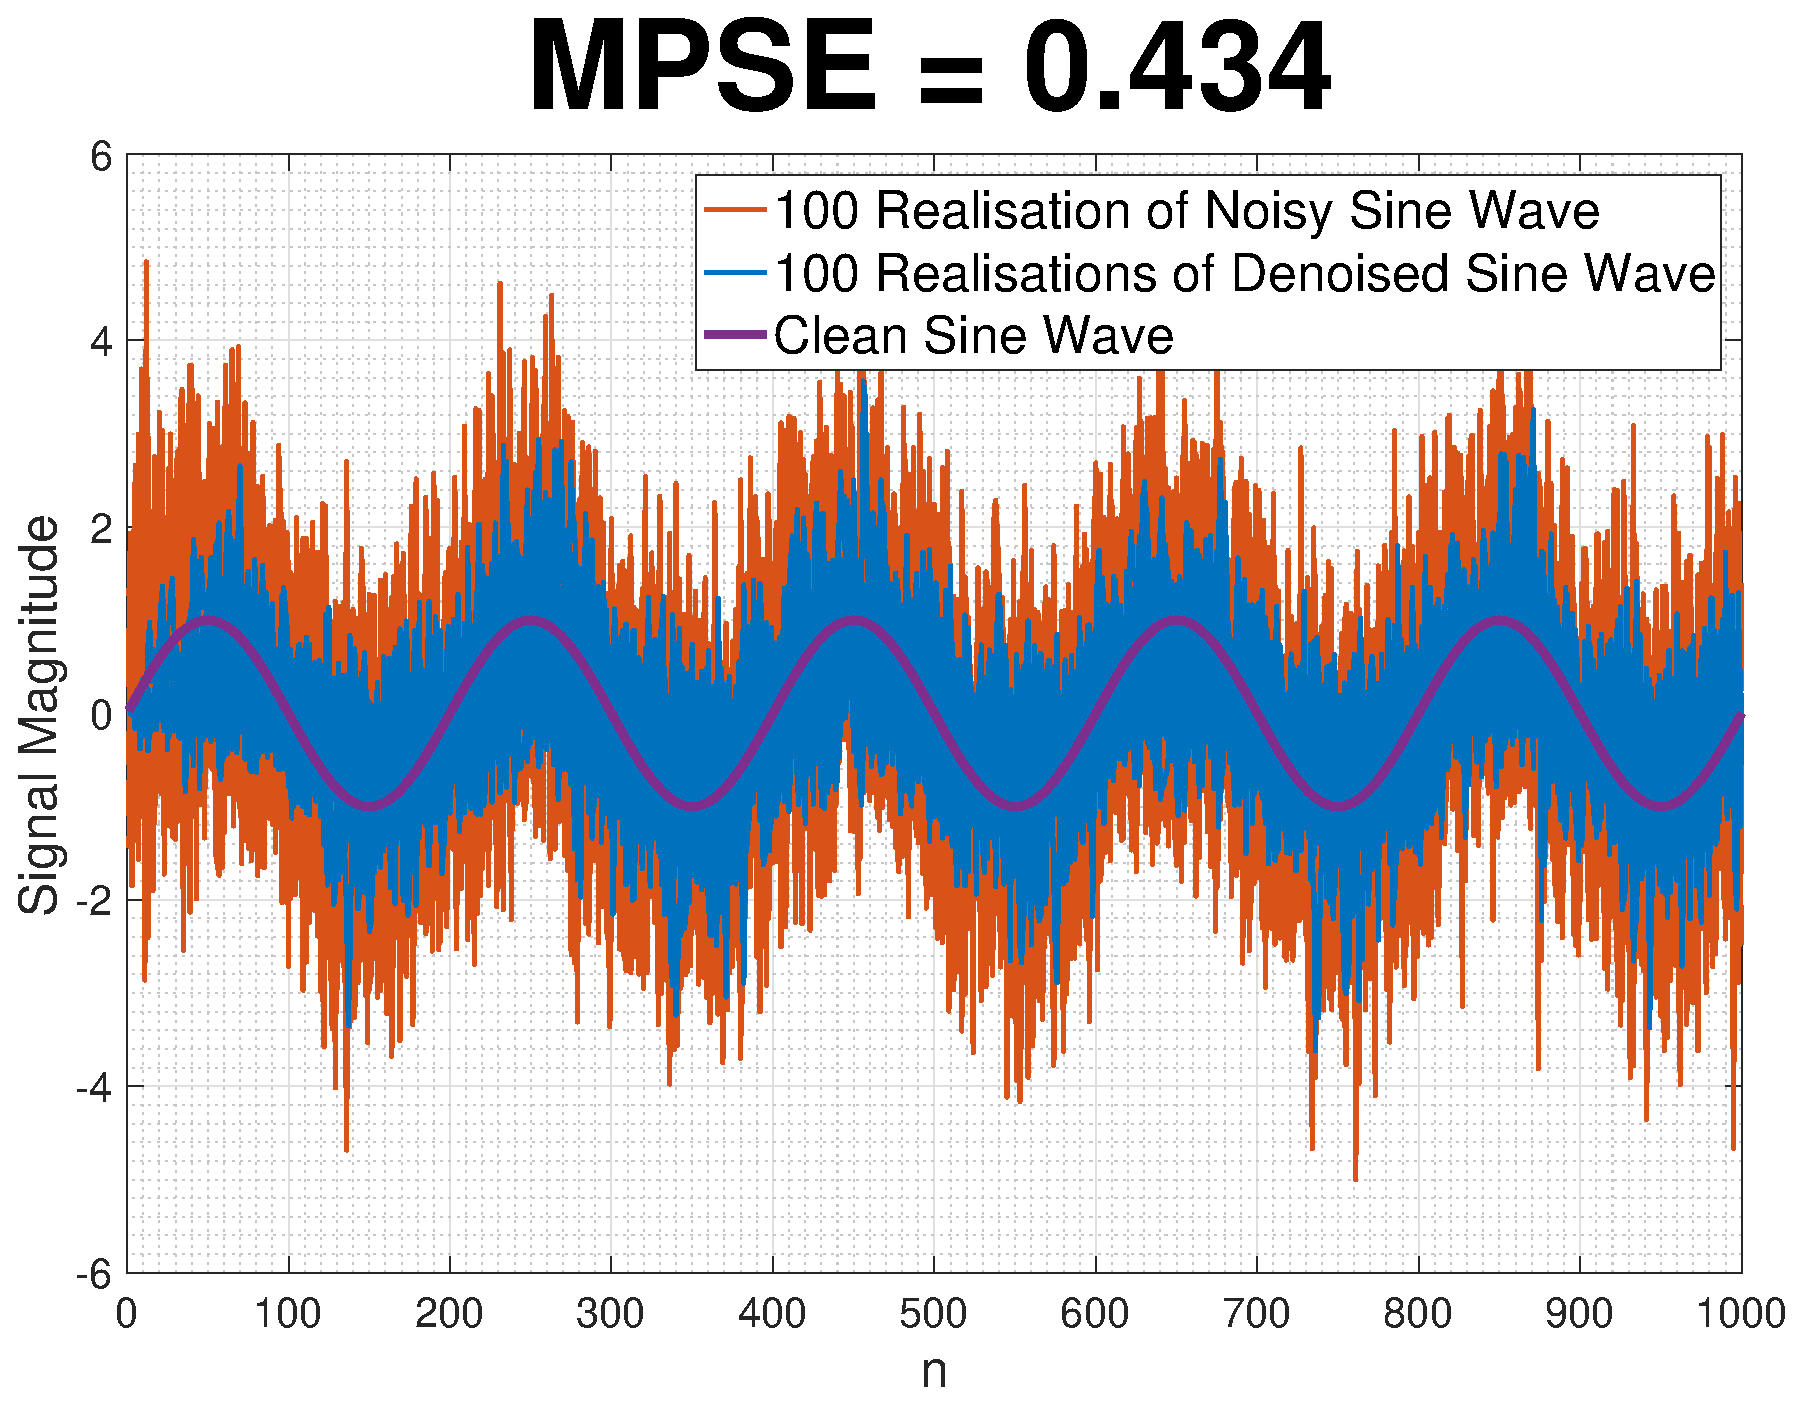
\includegraphics[width=0.24\textwidth]{part3/mpse_delay_1}
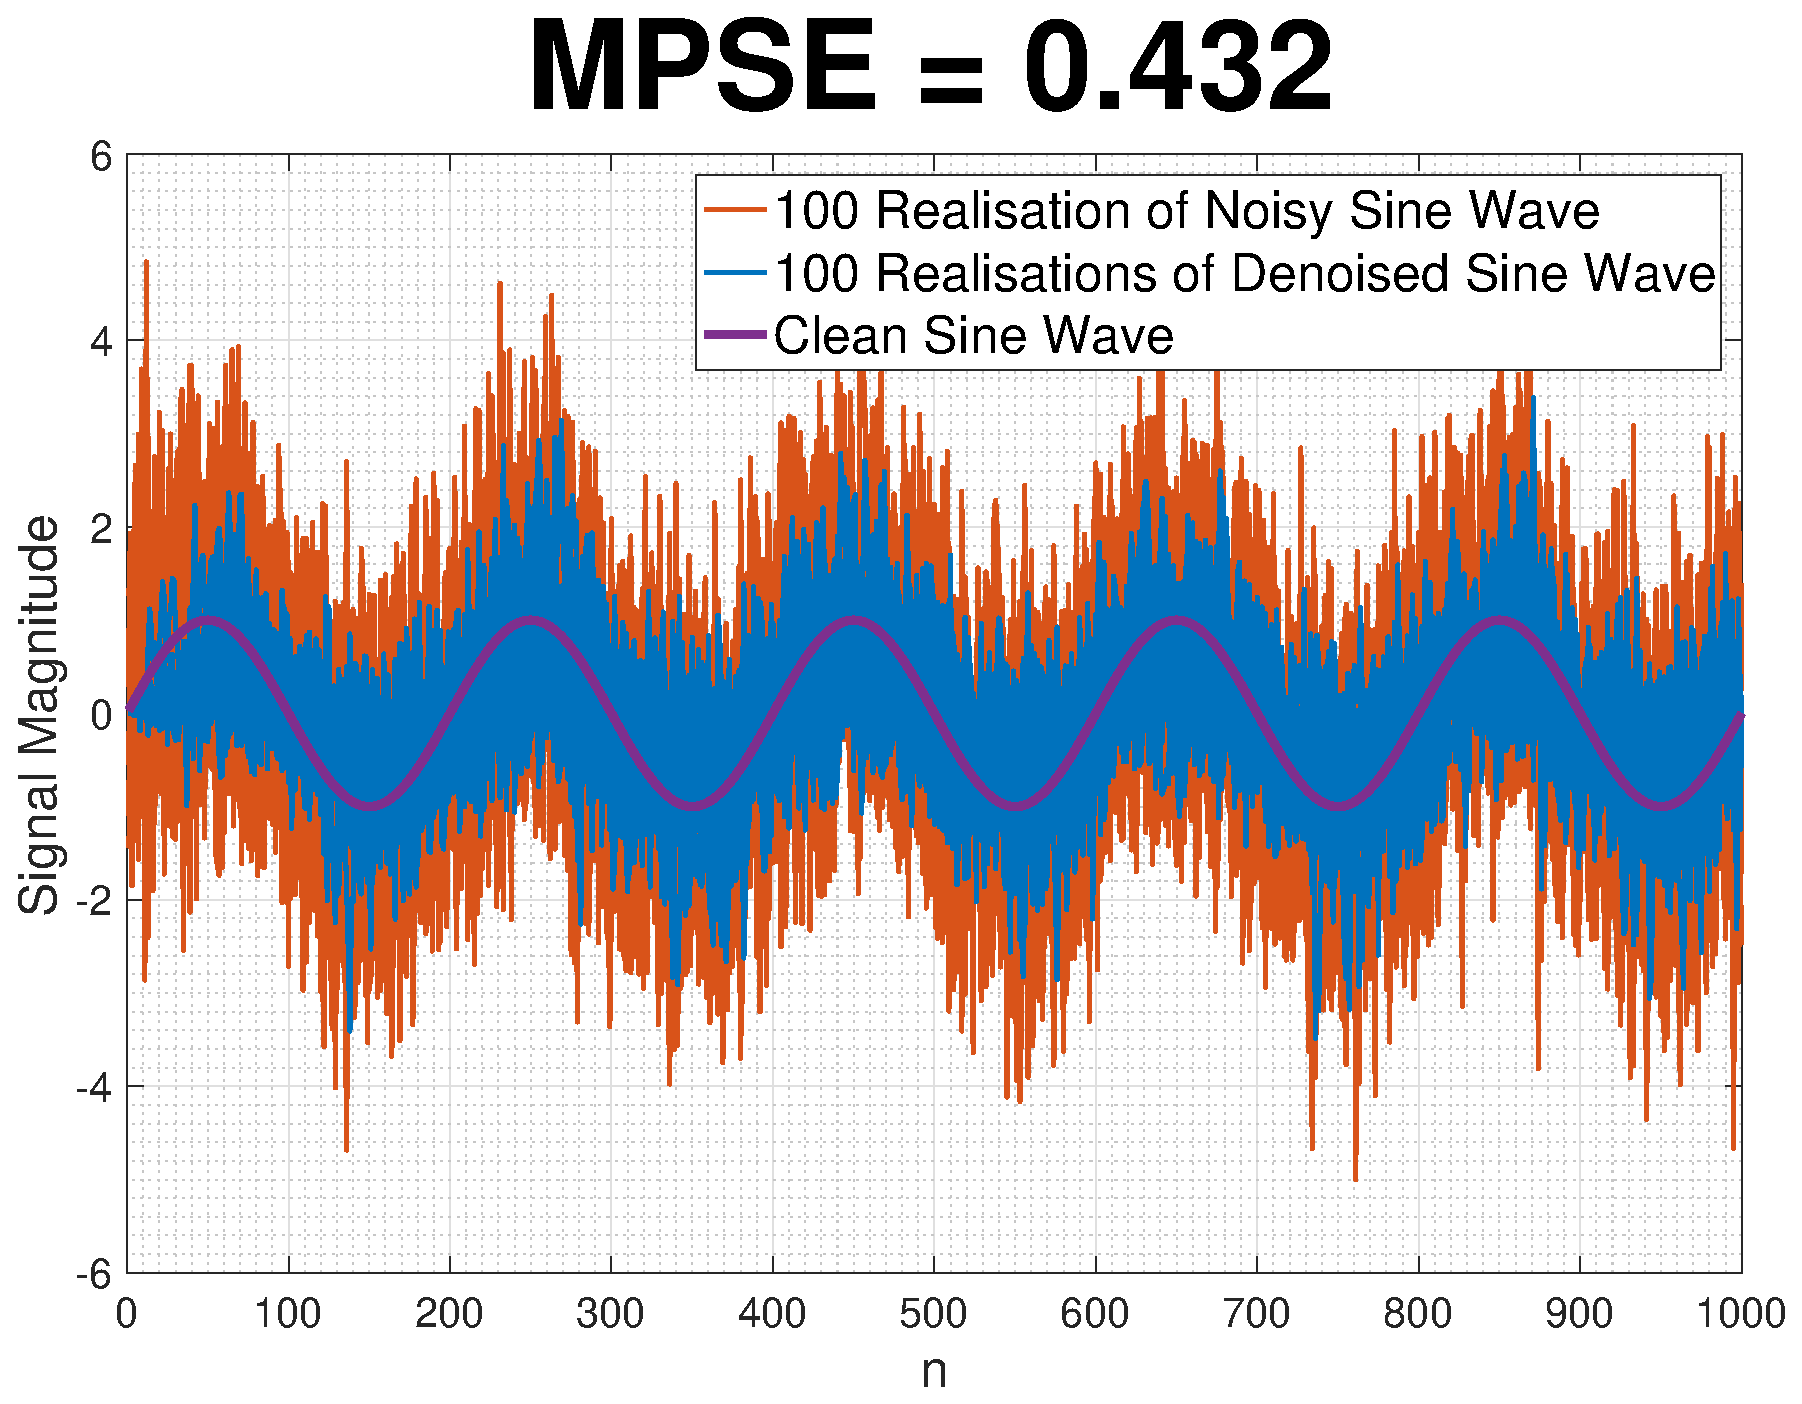
\includegraphics[width=0.24\textwidth]{part3/mpse_delay_2}
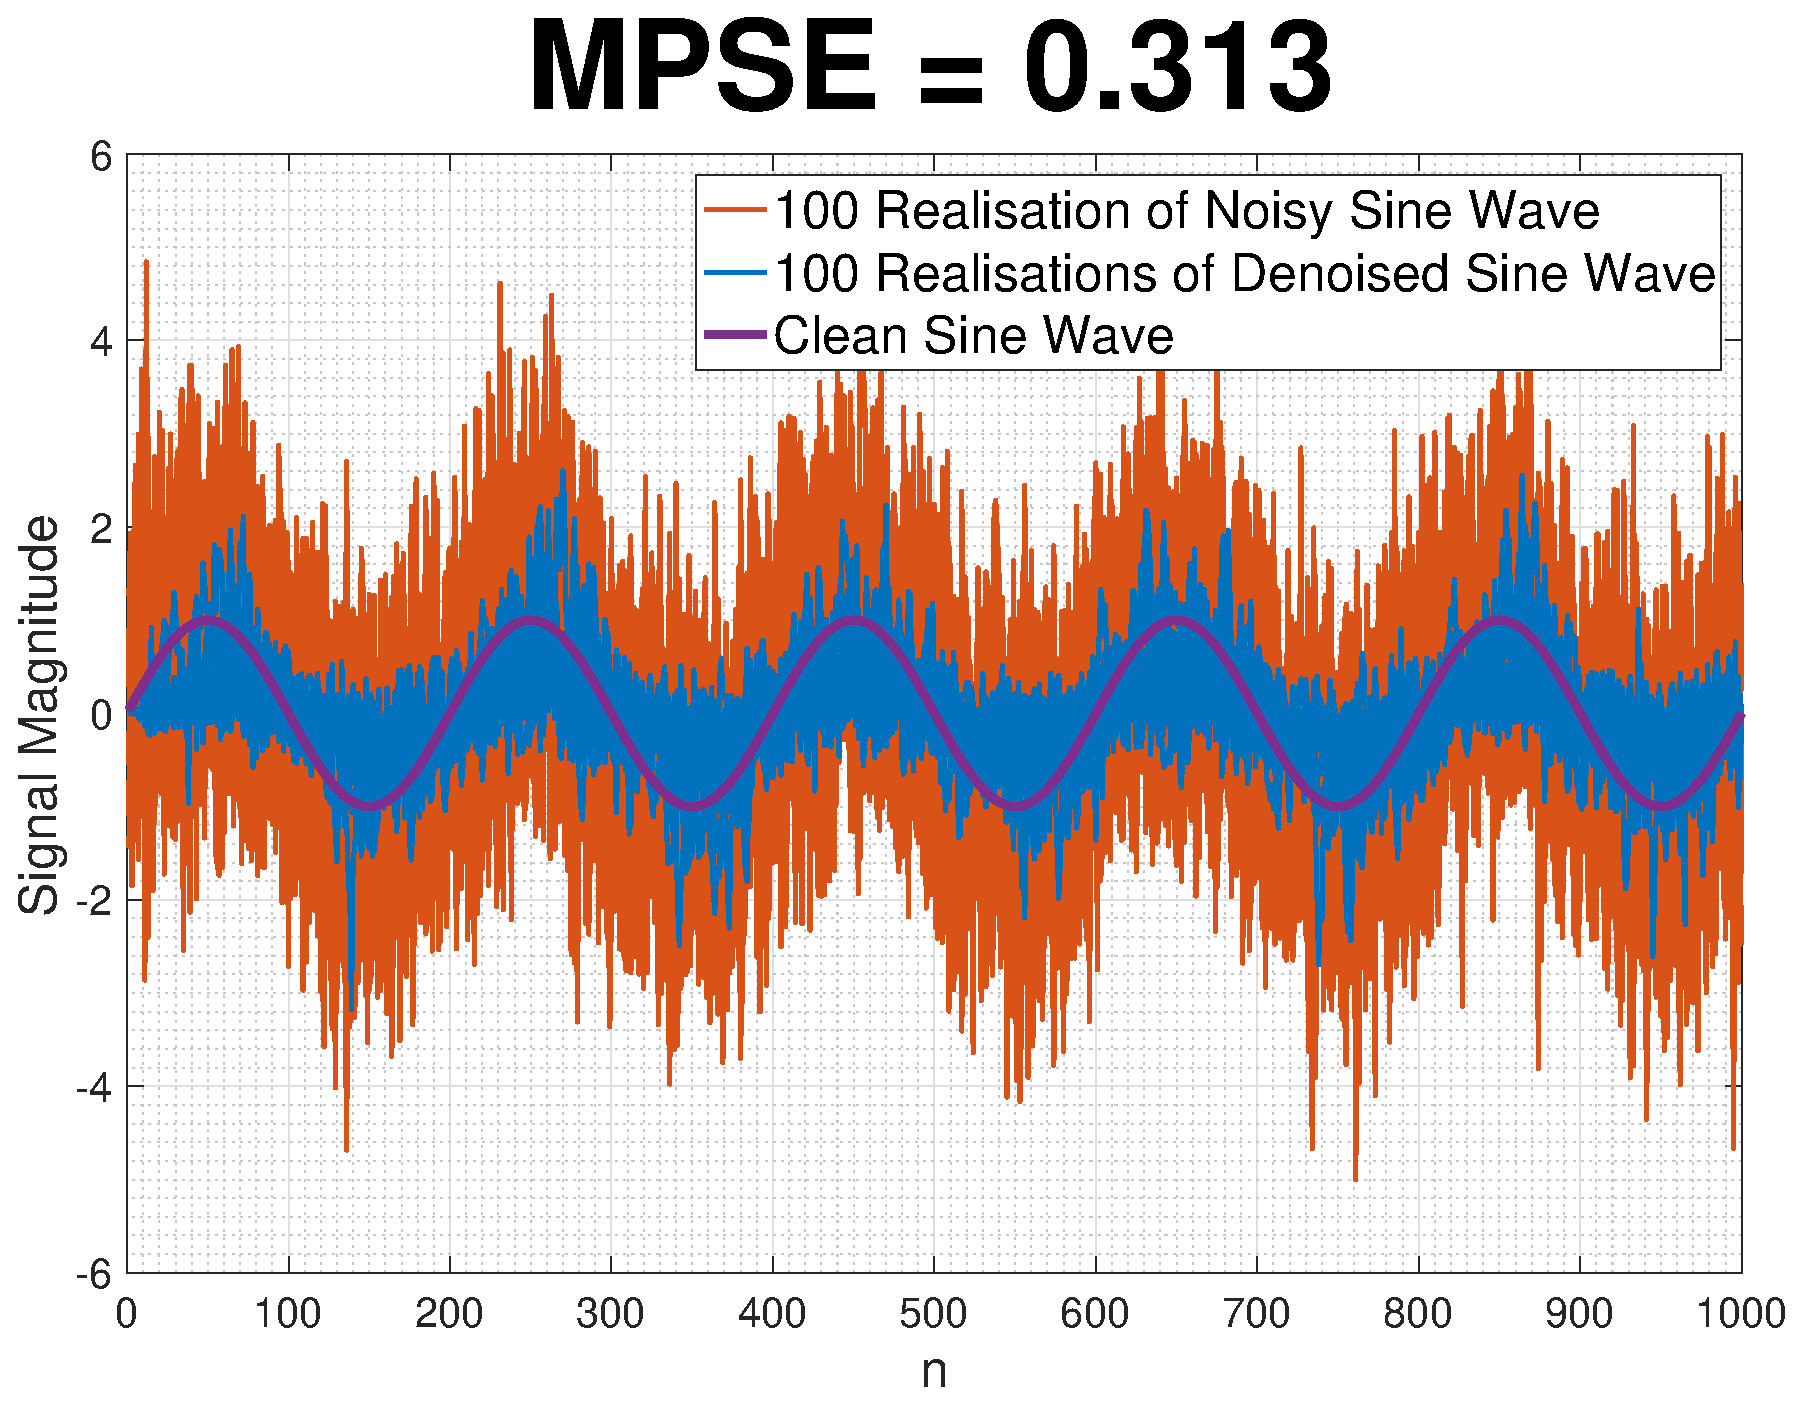
\includegraphics[width=0.24\textwidth]{part3/mpse_delay_3}
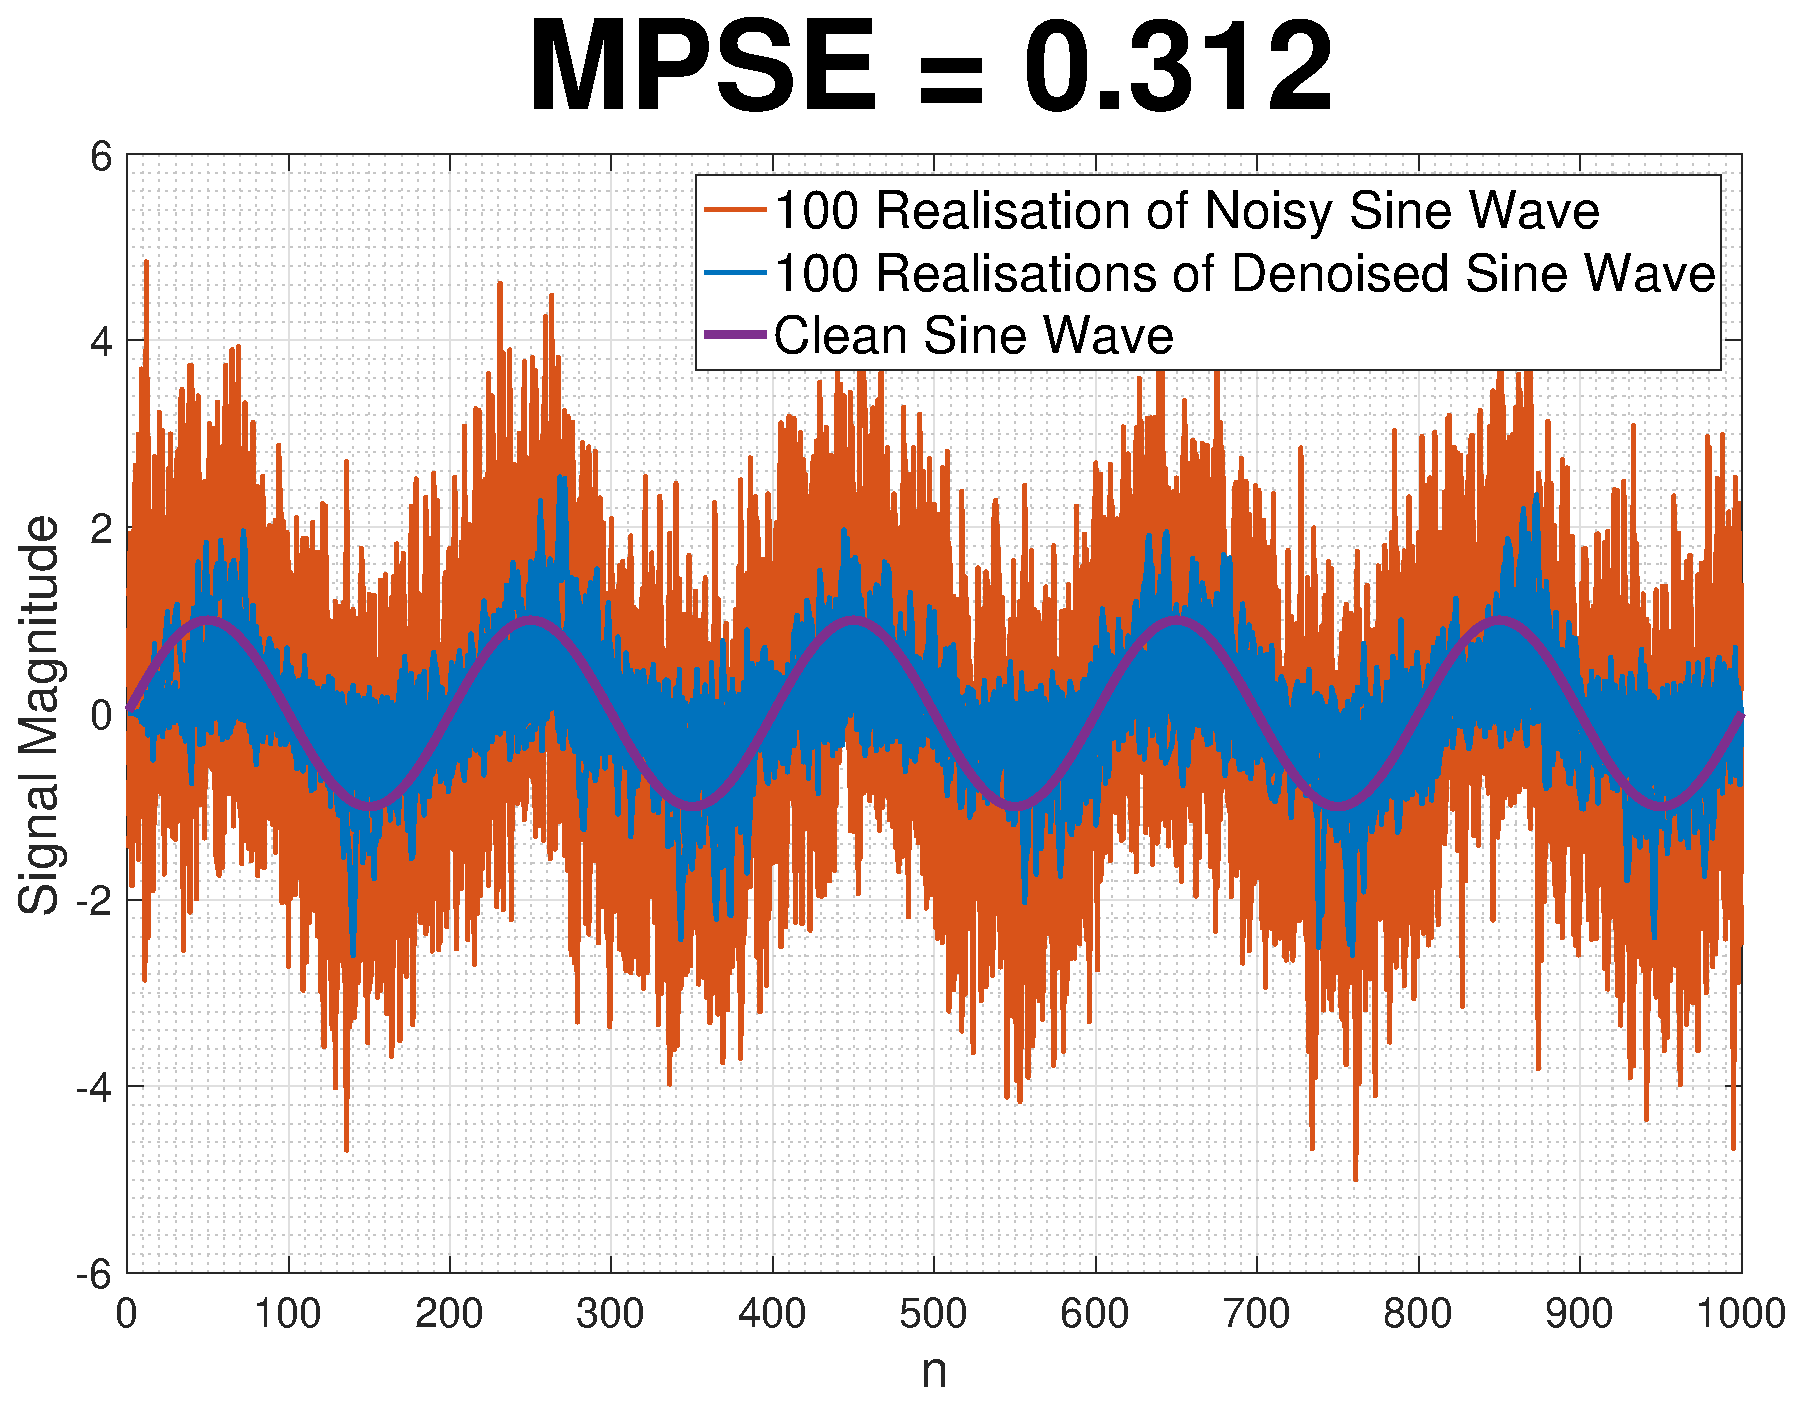
\includegraphics[width=0.24\textwidth]{part3/mpse_delay_4}
\caption{Determining Ideal Value for $\Delta$ to be used in the Adaptive Line Enhancement Algorithm}
\end{figure}

\begin{figure}[H]
\centering{}
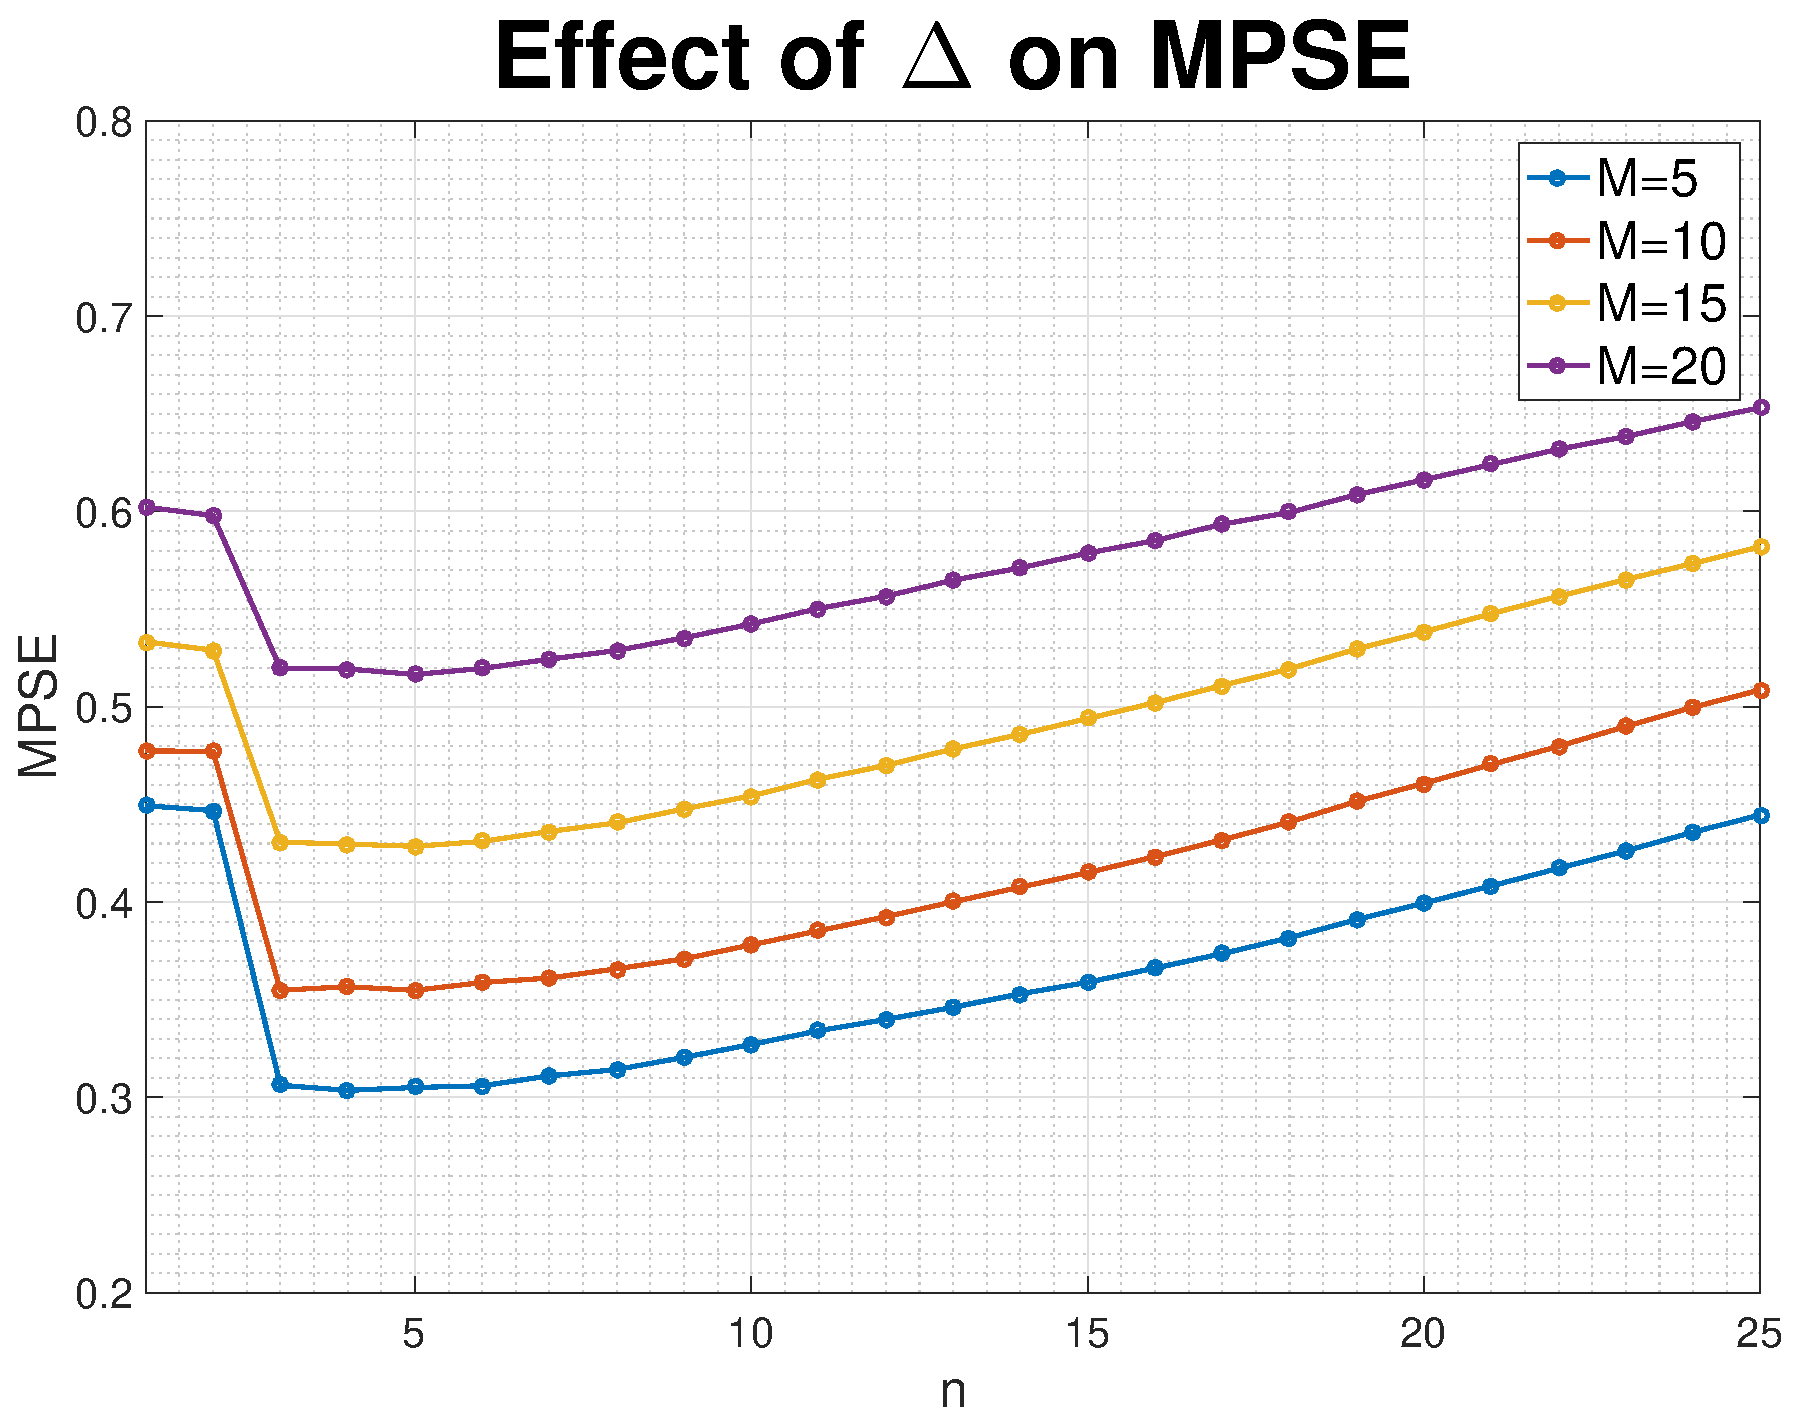
\includegraphics[width=0.32\textwidth]{part3/delay_vs_mpse}
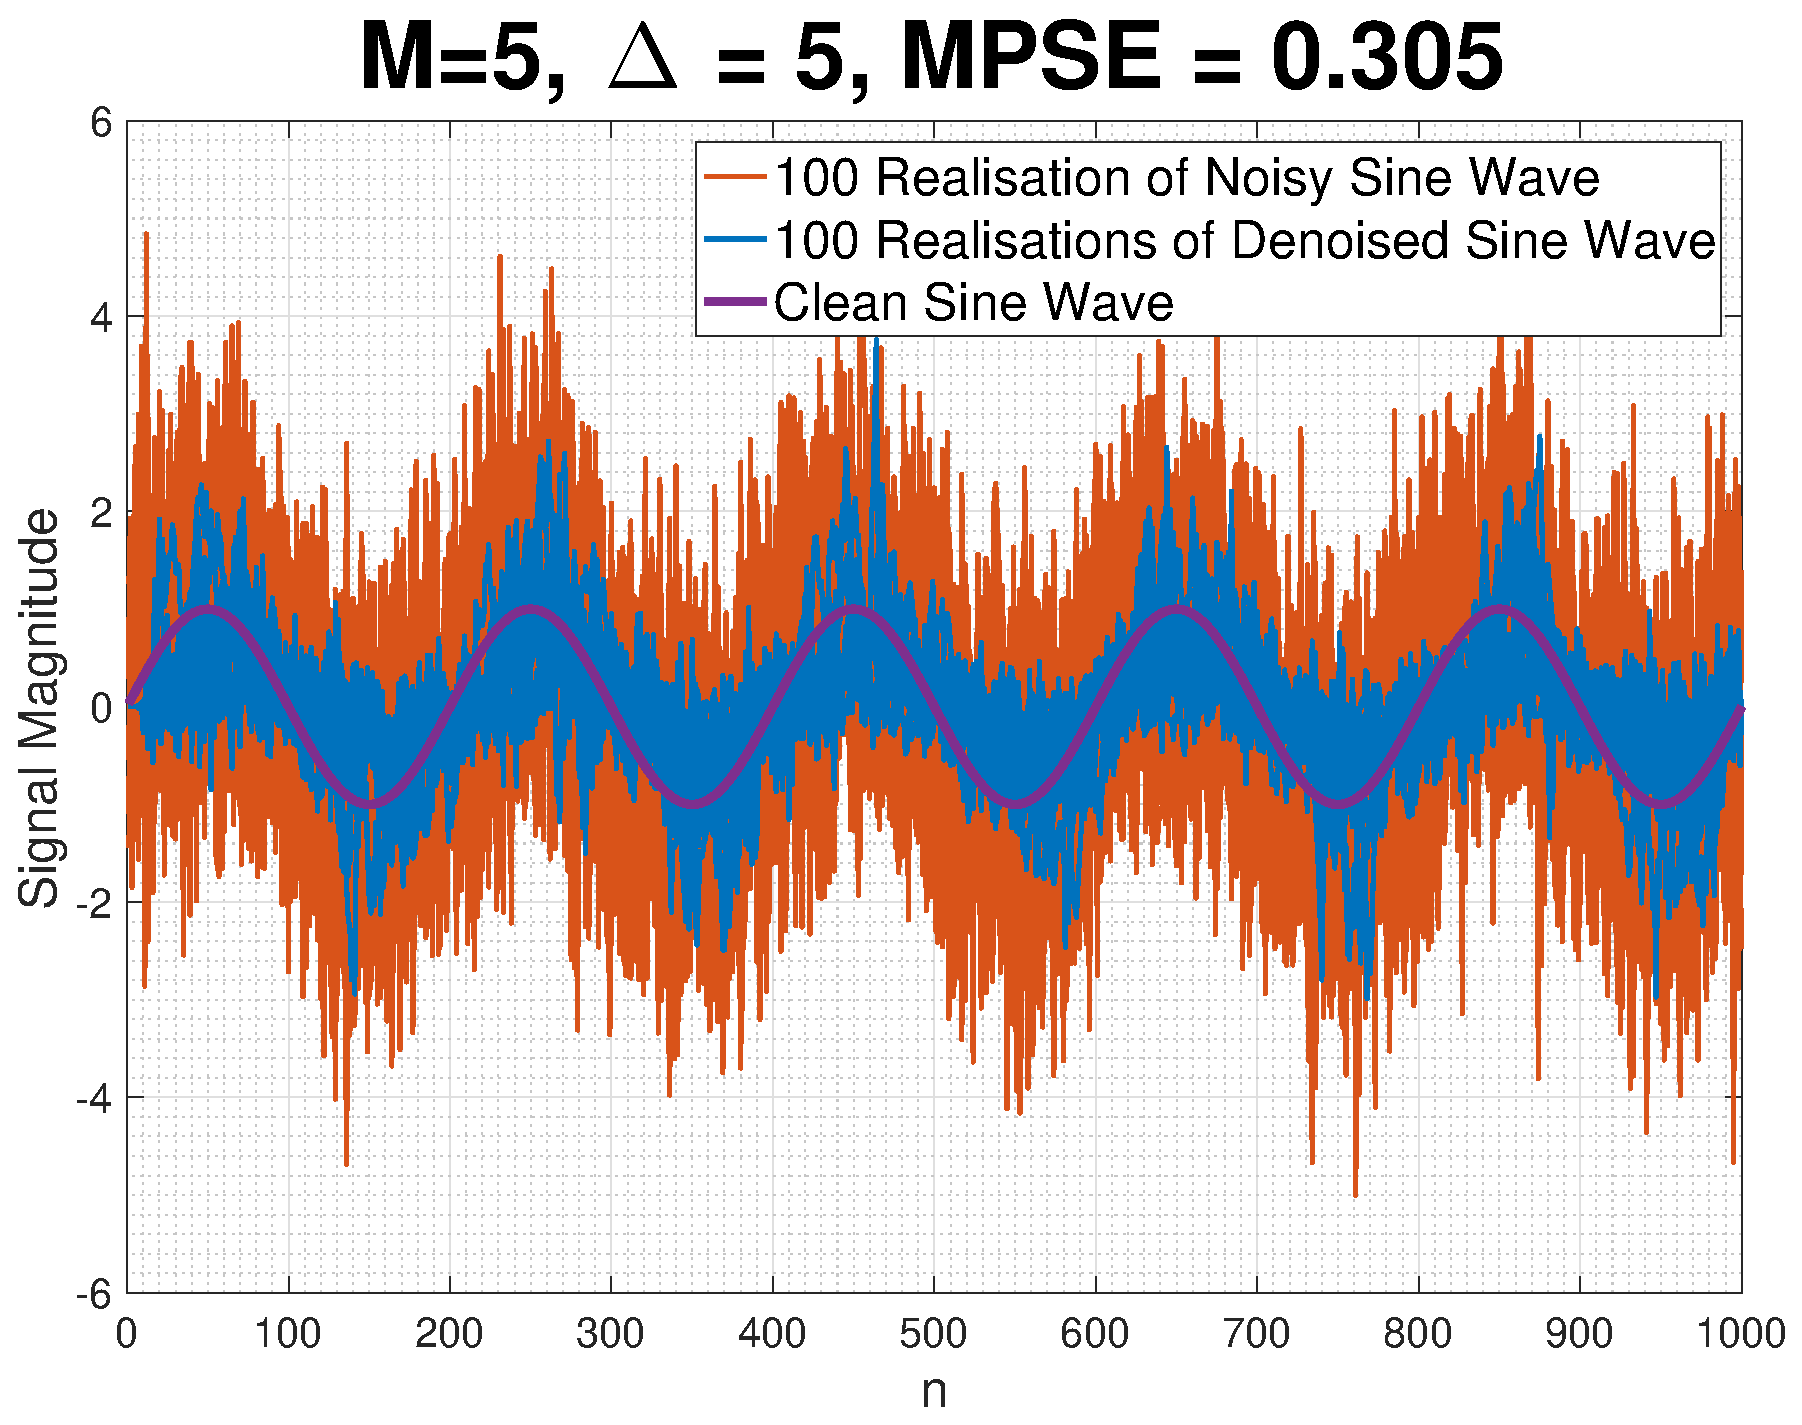
\includegraphics[width=0.32\textwidth]{part3/mpse_delay_5}
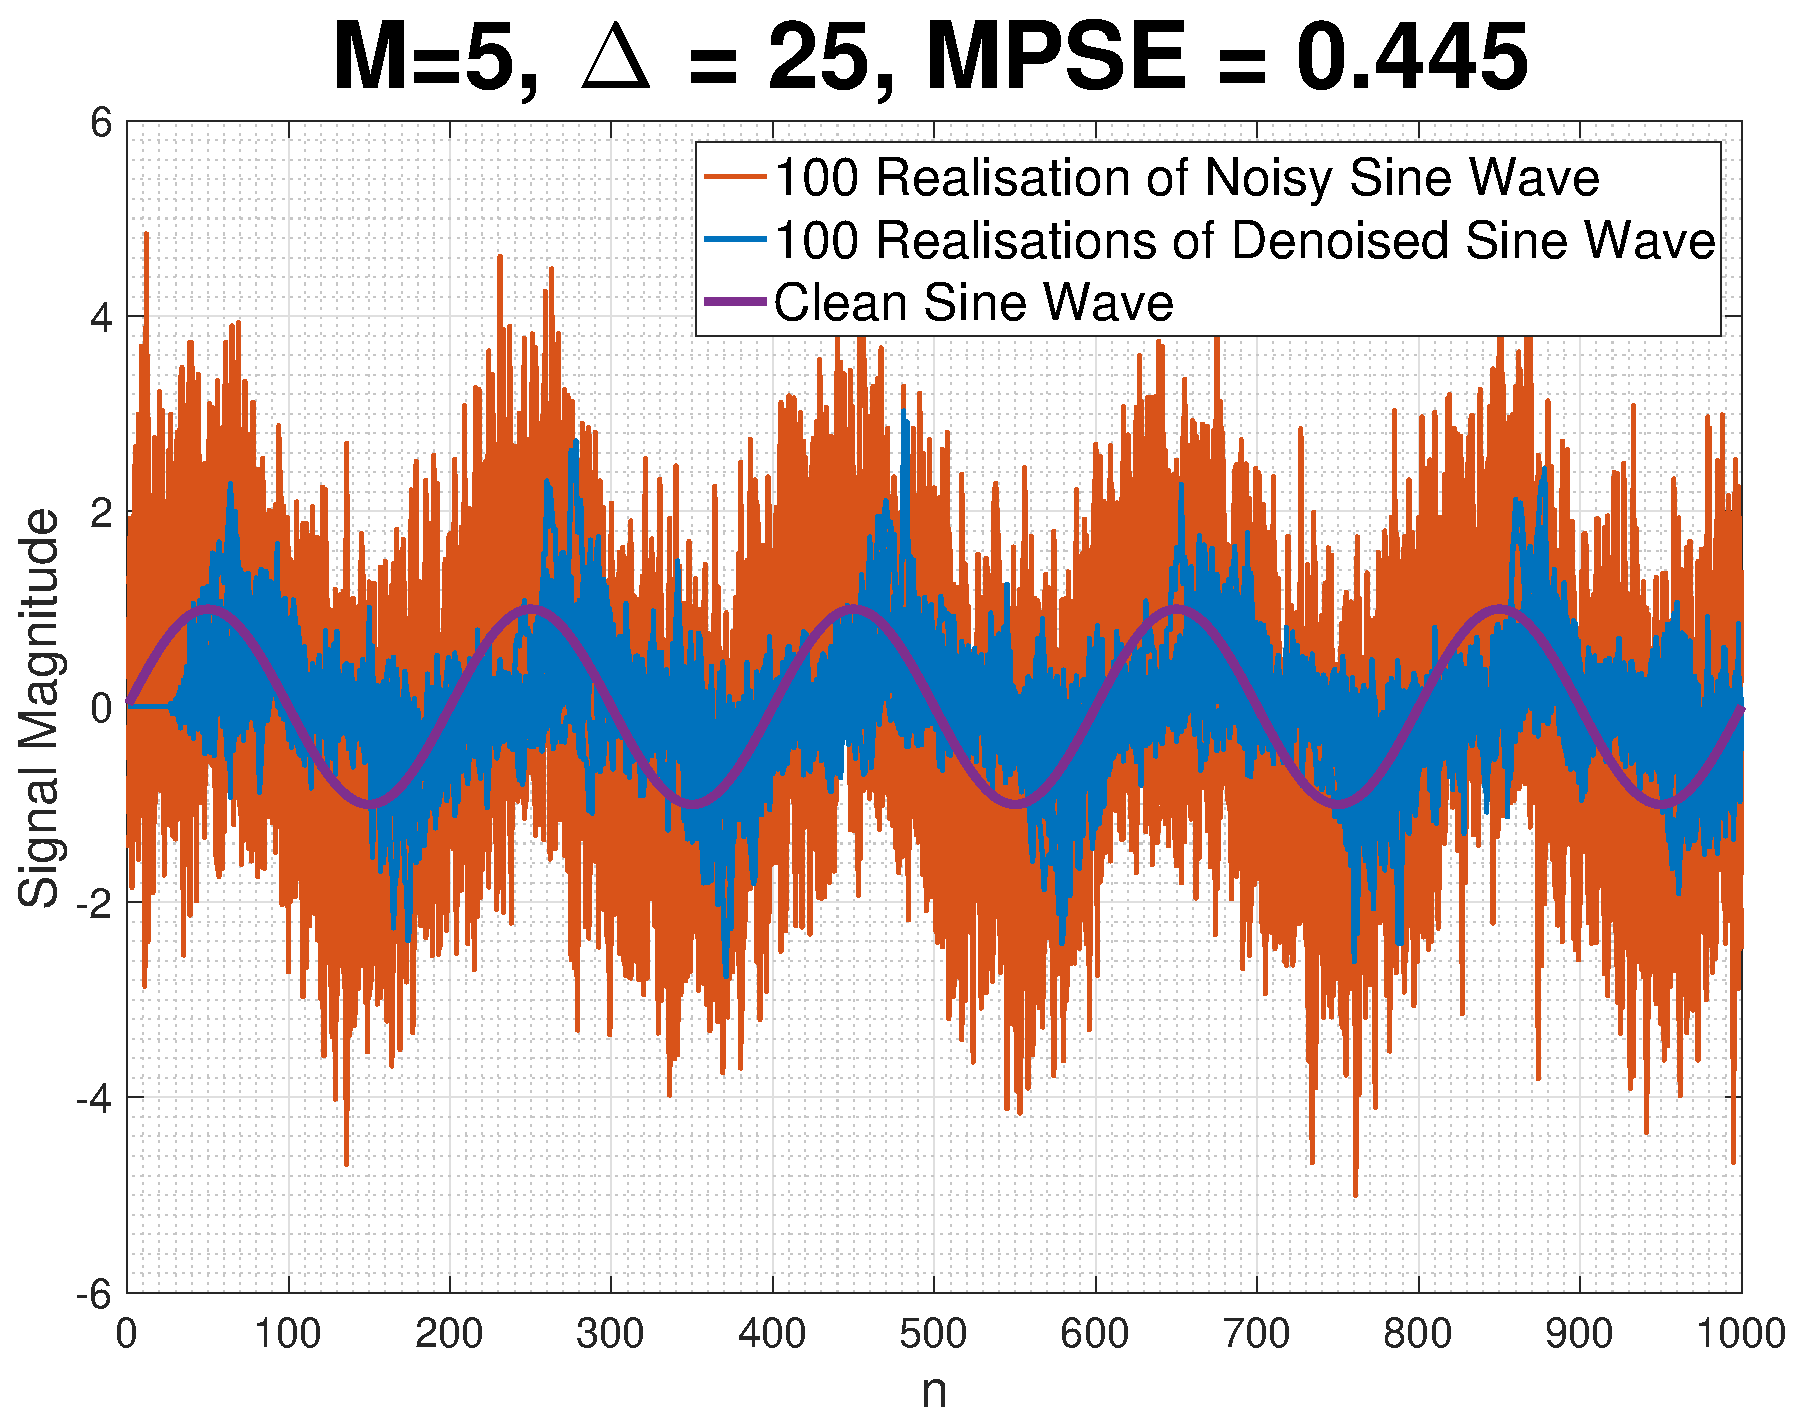
\includegraphics[width=0.32\textwidth]{part3/mpse_delay_25}
\caption{Studying the Effects of Increasing Delay on the MPSE}
\end{figure}

\begin{figure}[H]
\centering{}
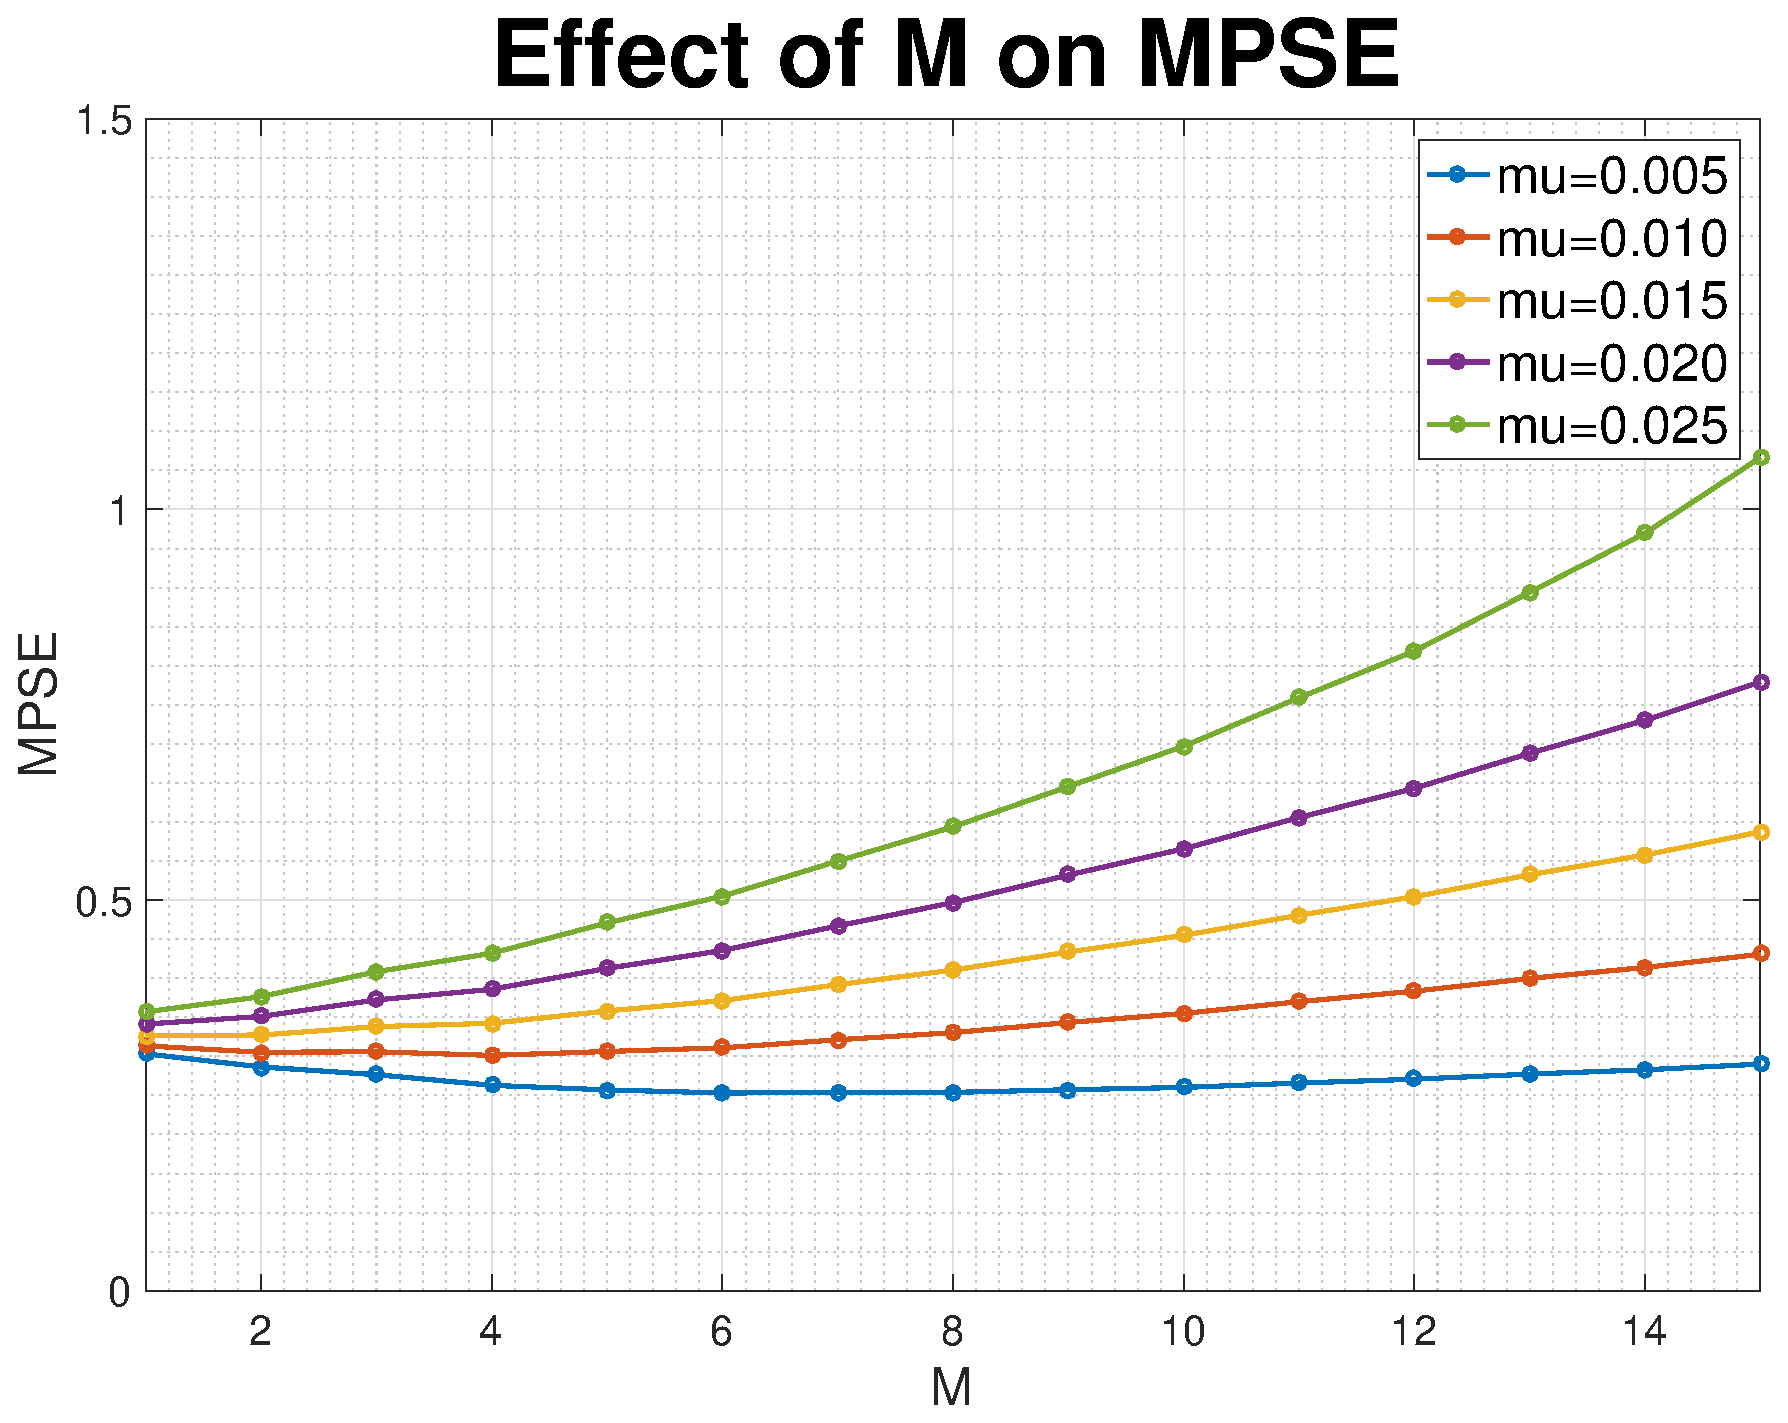
\includegraphics[width=0.32\textwidth]{part3/model_order_mpse}
\caption{Studying the Effects of Increasing Model Order on the MPSE}
\end{figure}

\begin{figure}[H]
\centering{}
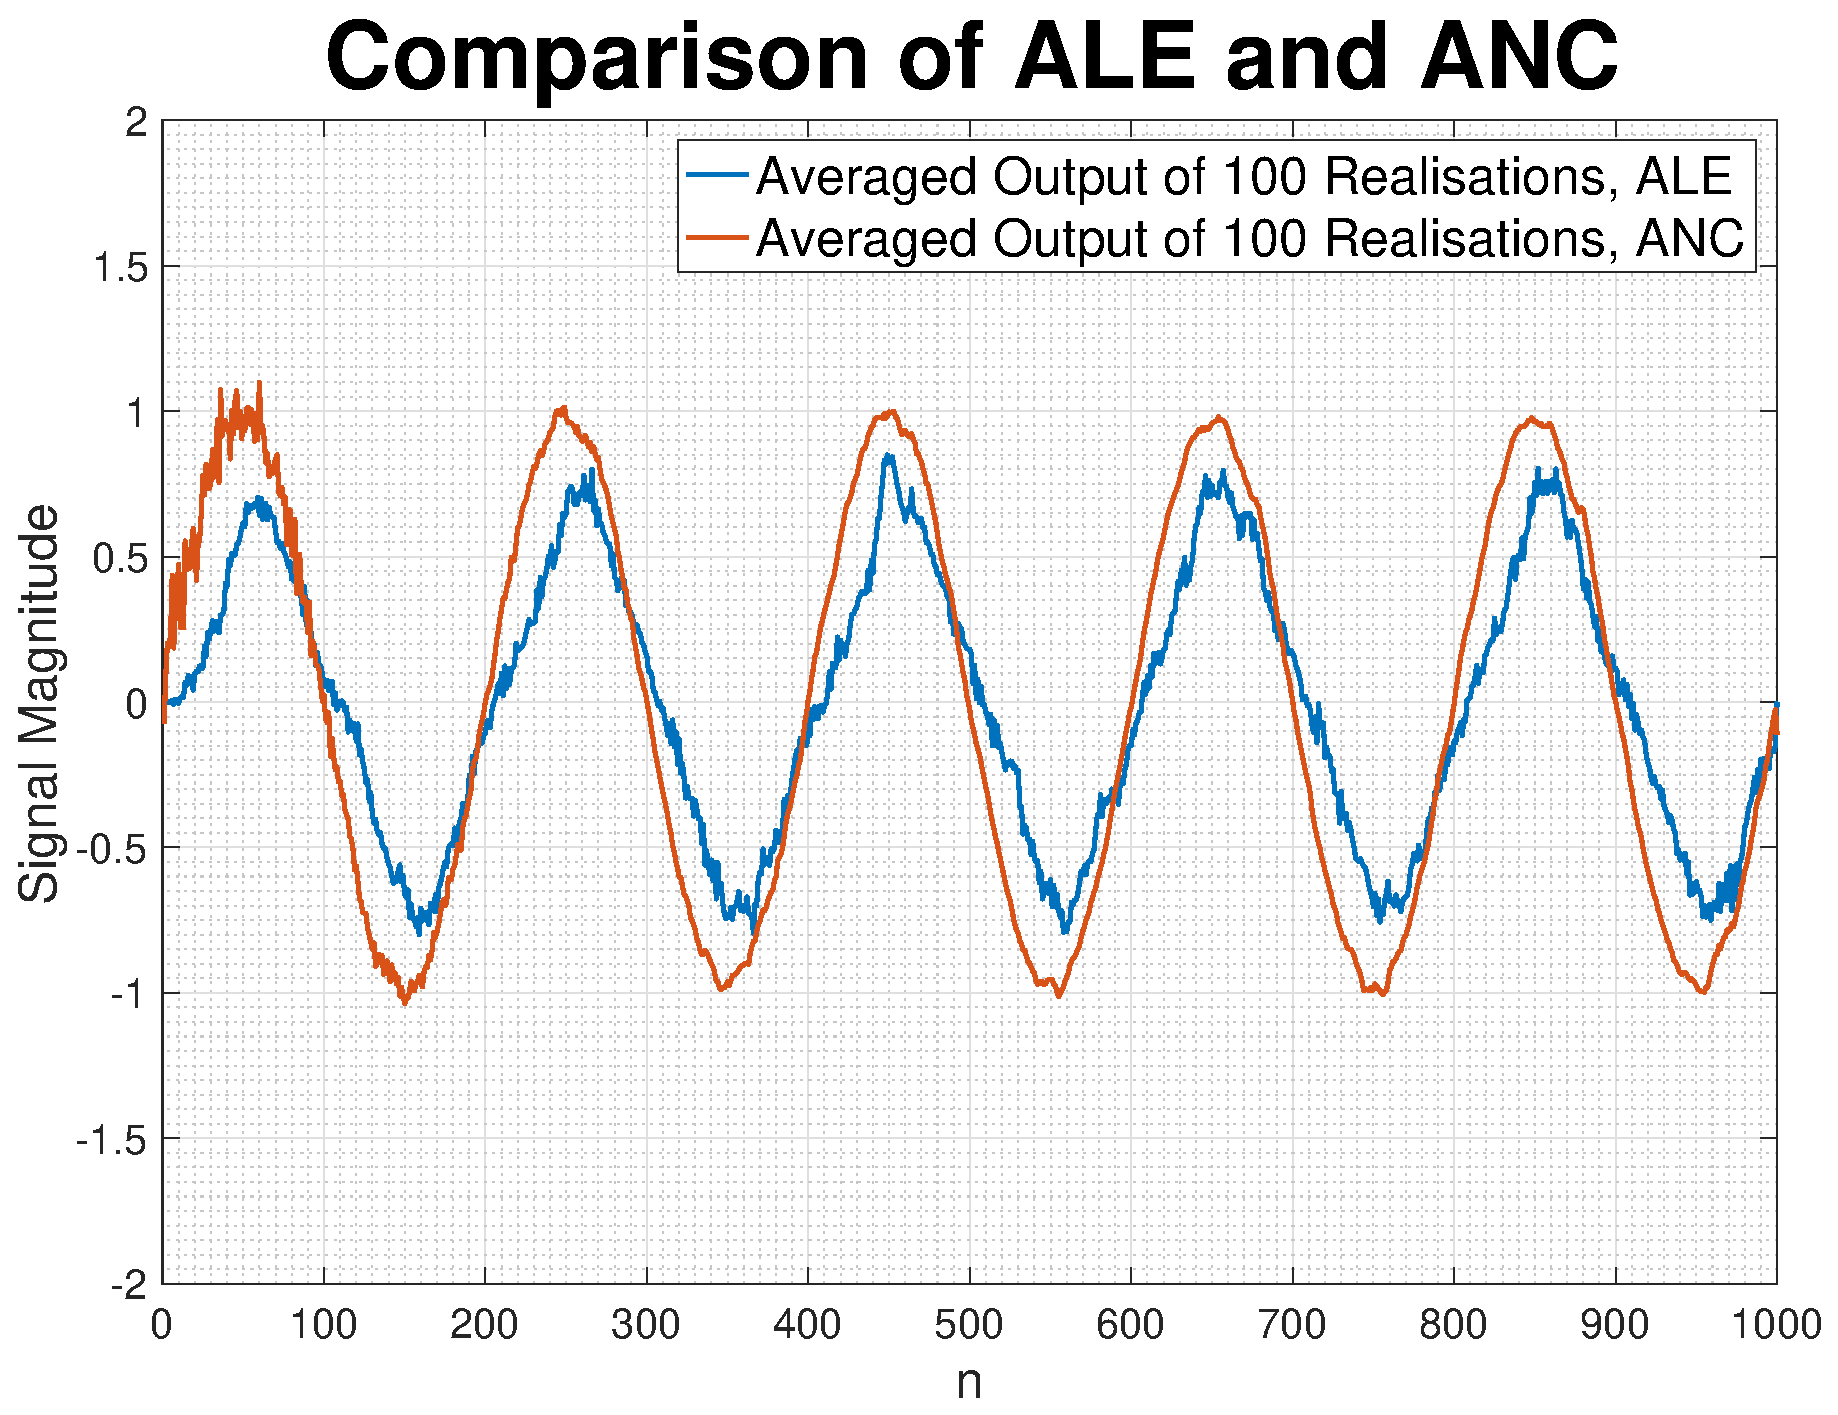
\includegraphics[width=0.32\textwidth]{part3/anc_ale_comparison}
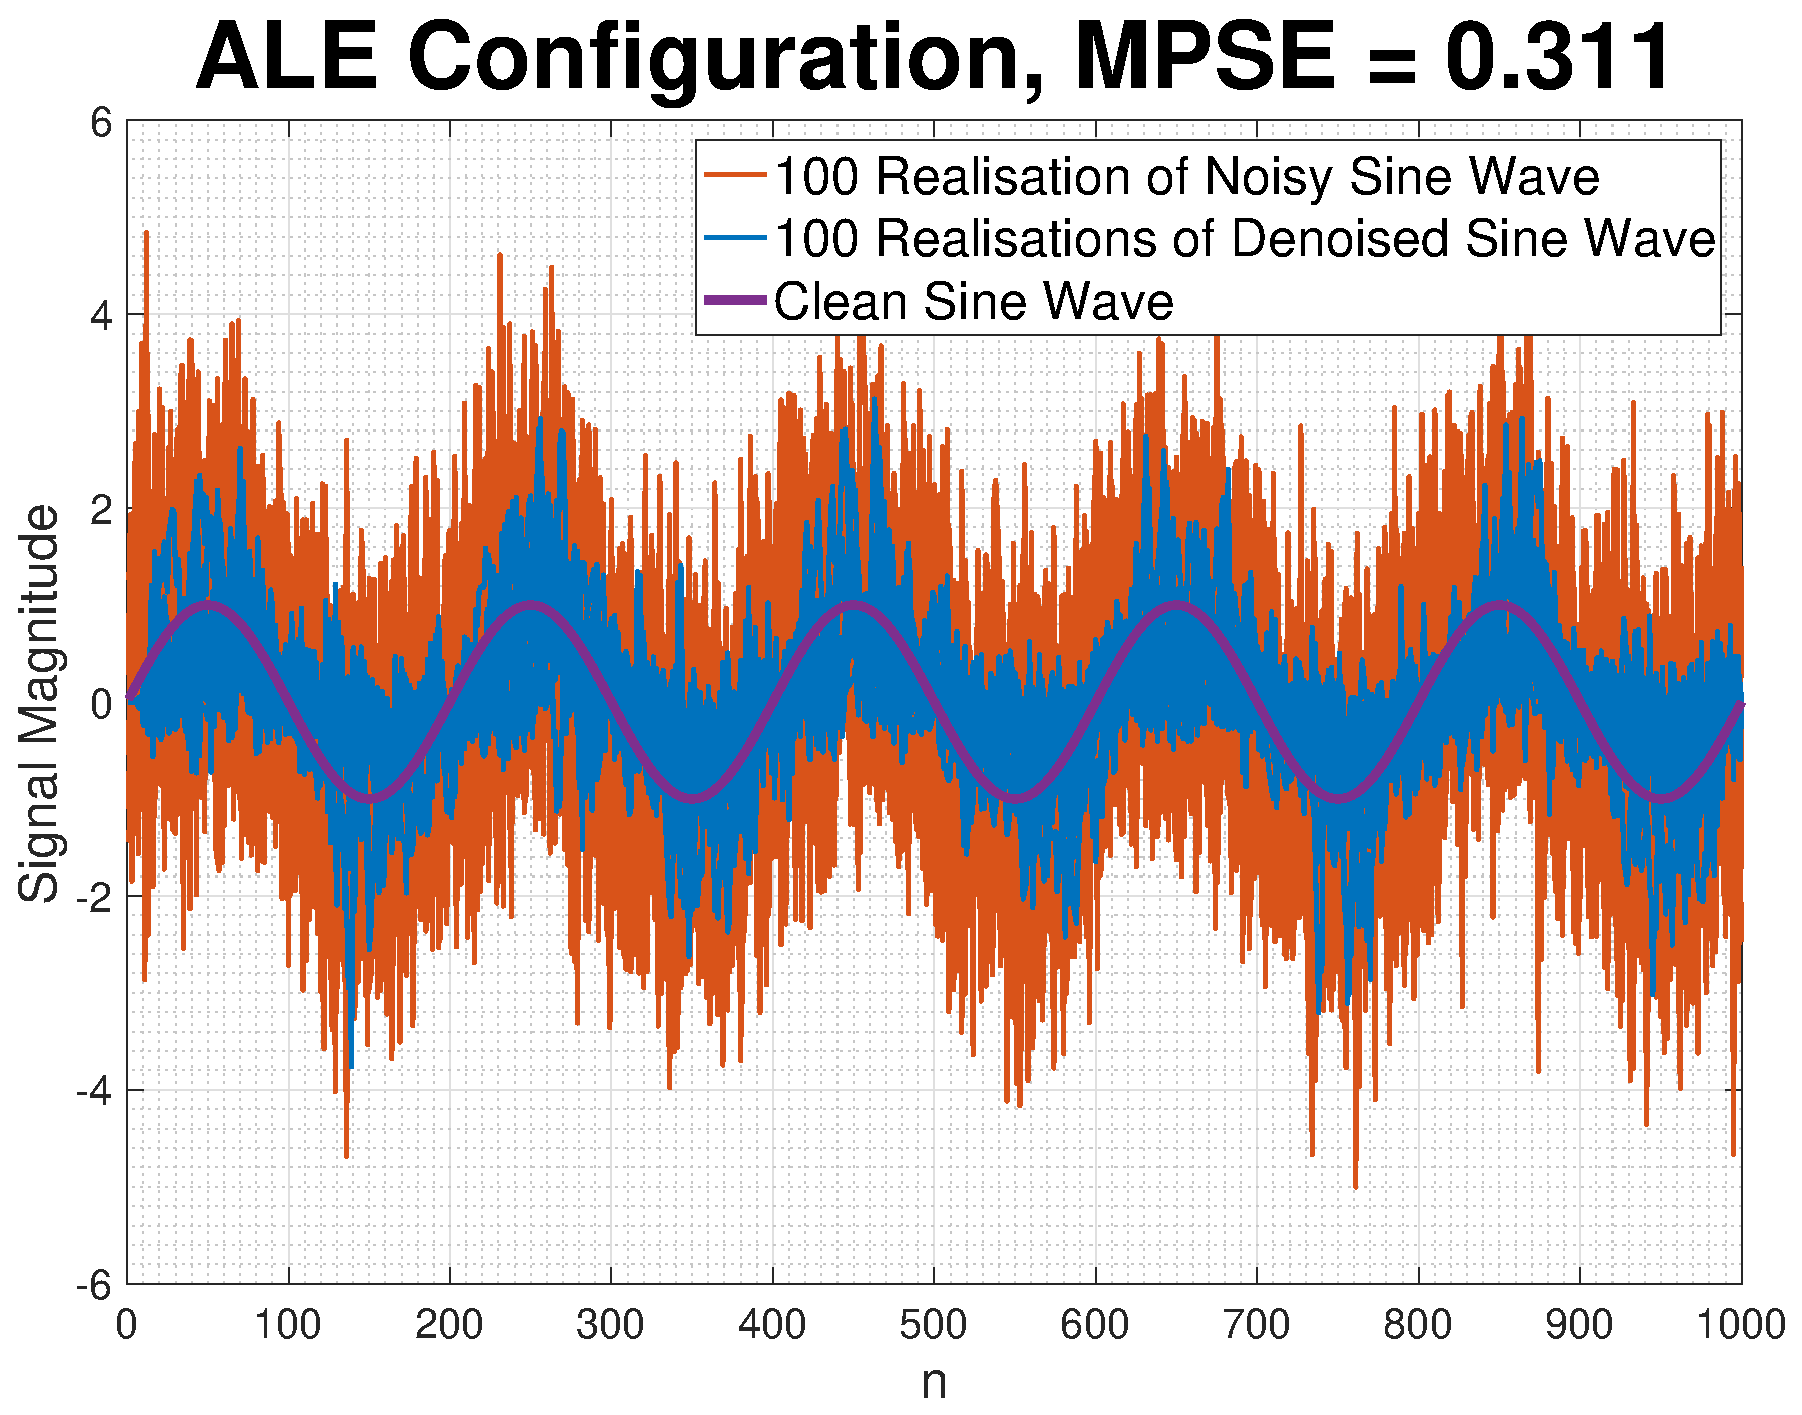
\includegraphics[width=0.32\textwidth]{part3/ale_mpse}
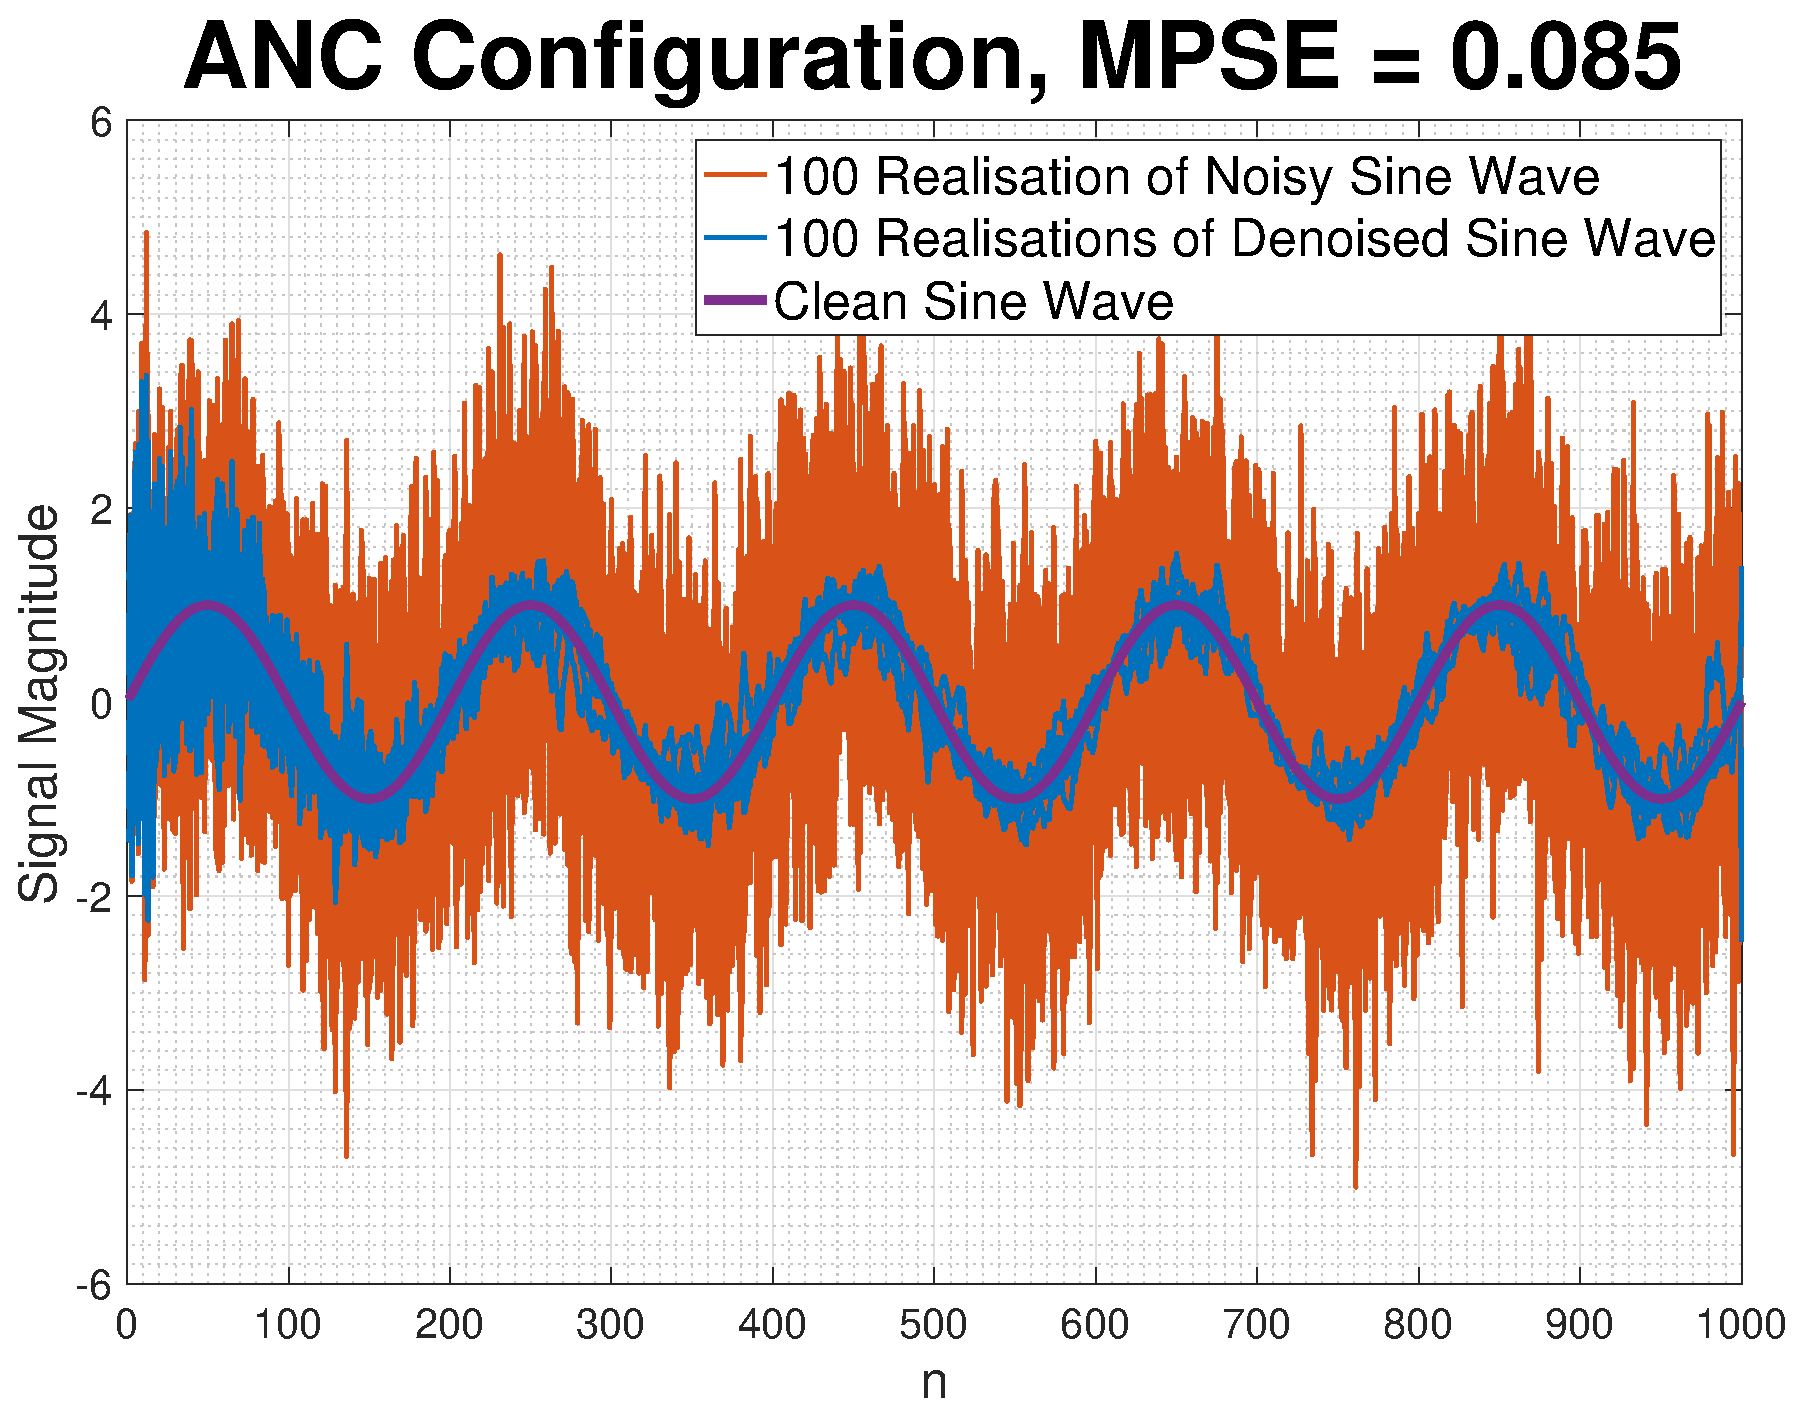
\includegraphics[width=0.32\textwidth]{part3/anc_mpse}
\caption{Comparison of ALE and ANC Configurations for Denoising Sinewave}
\end{figure}

\begin{figure}[H]
\centering{}
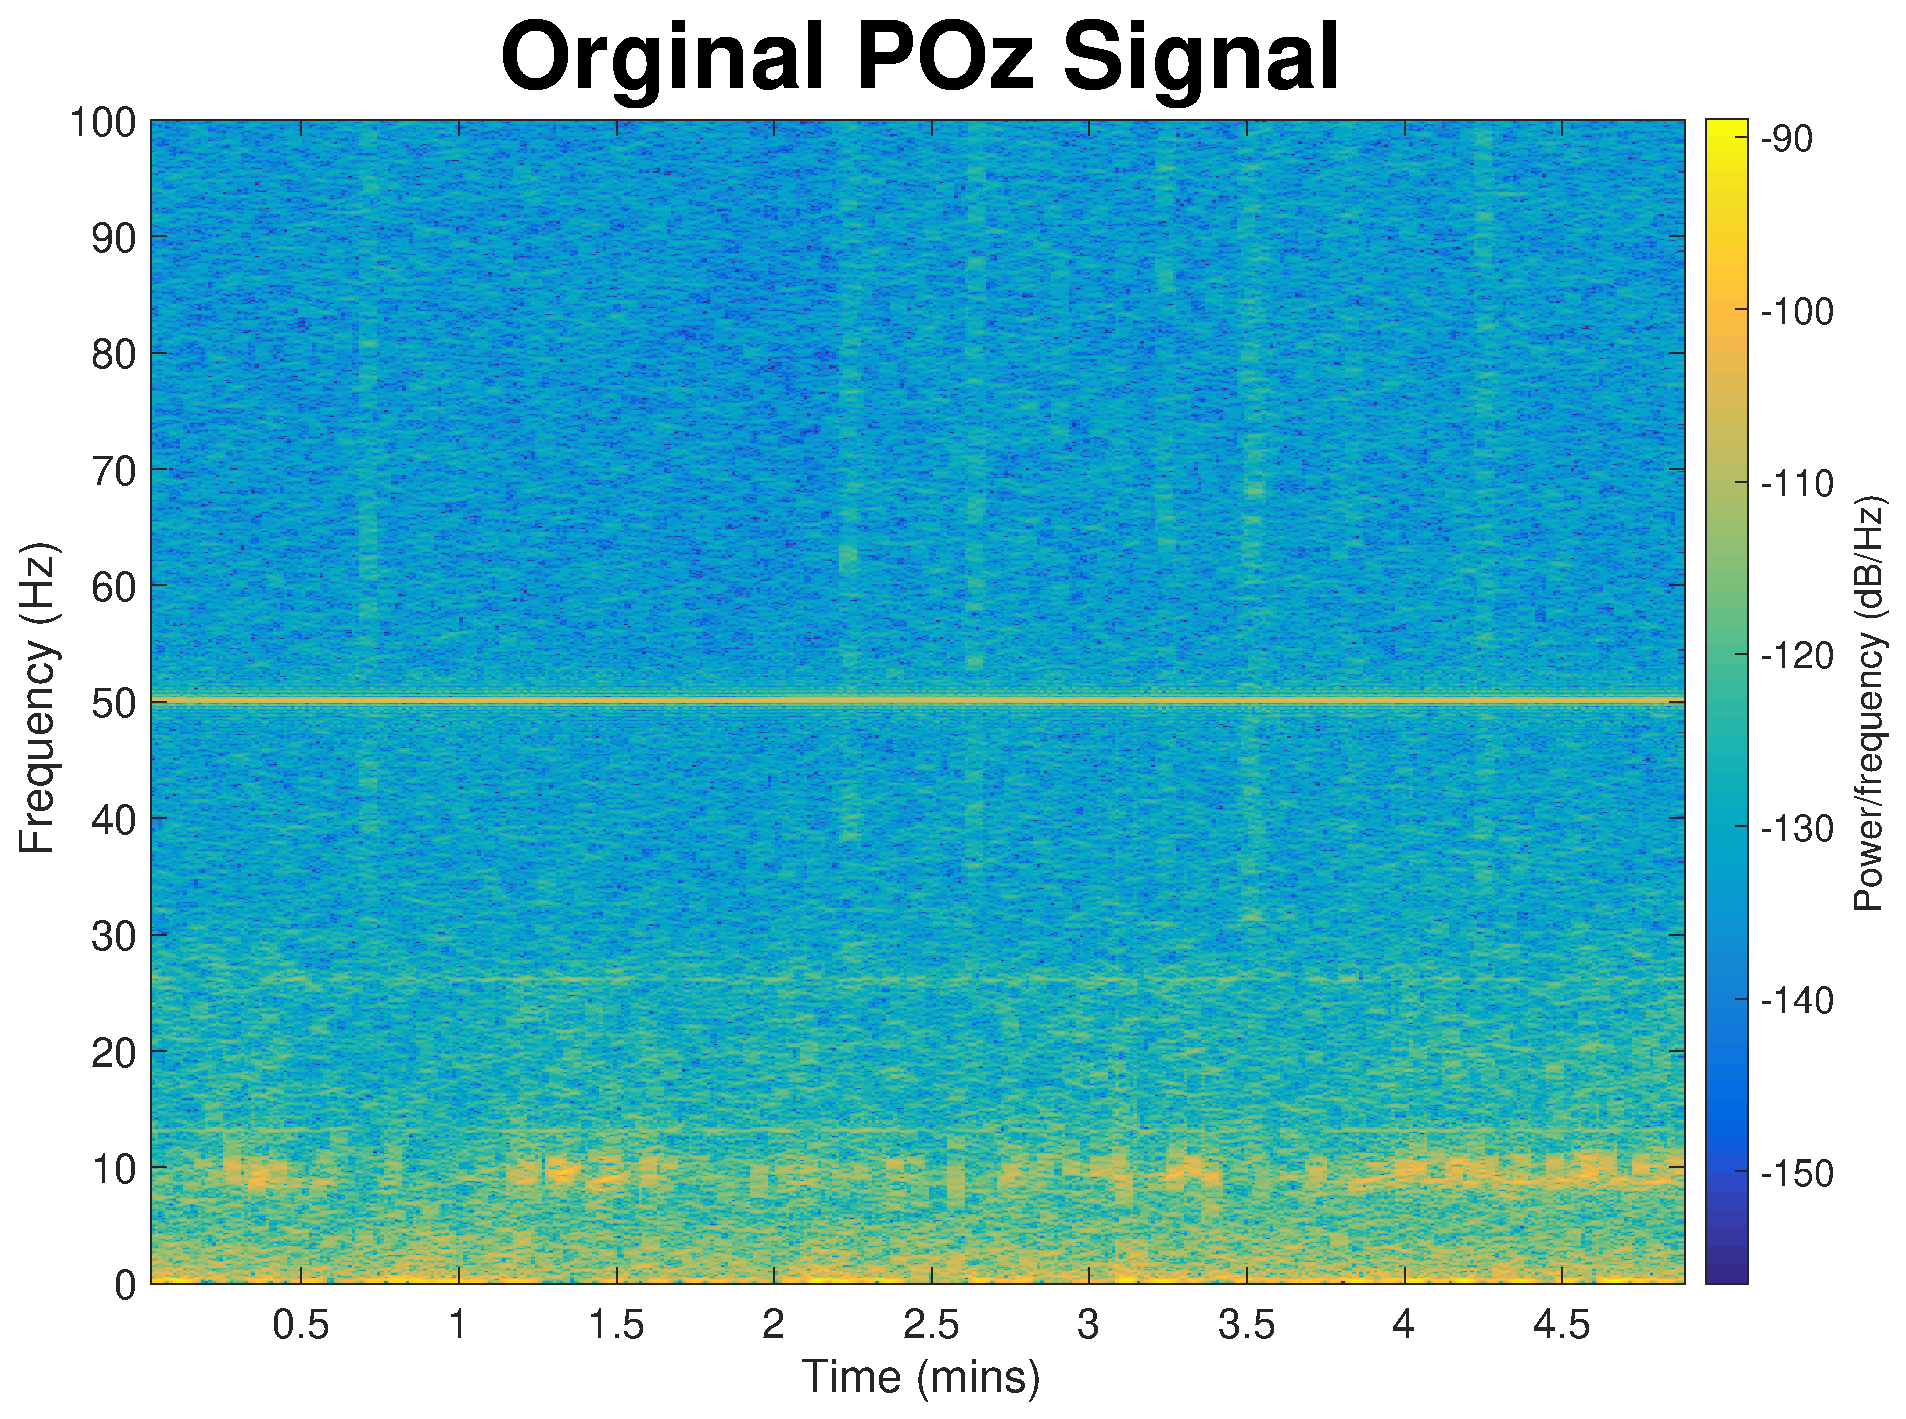
\includegraphics[width=0.32\textwidth]{part3/original_POz_spectrogram}
\caption{Original EEG Data collected from POz Location on the Scalp with Strong Component at 50 Hz}
\end{figure}


\begin{figure}[H]
\centering{}
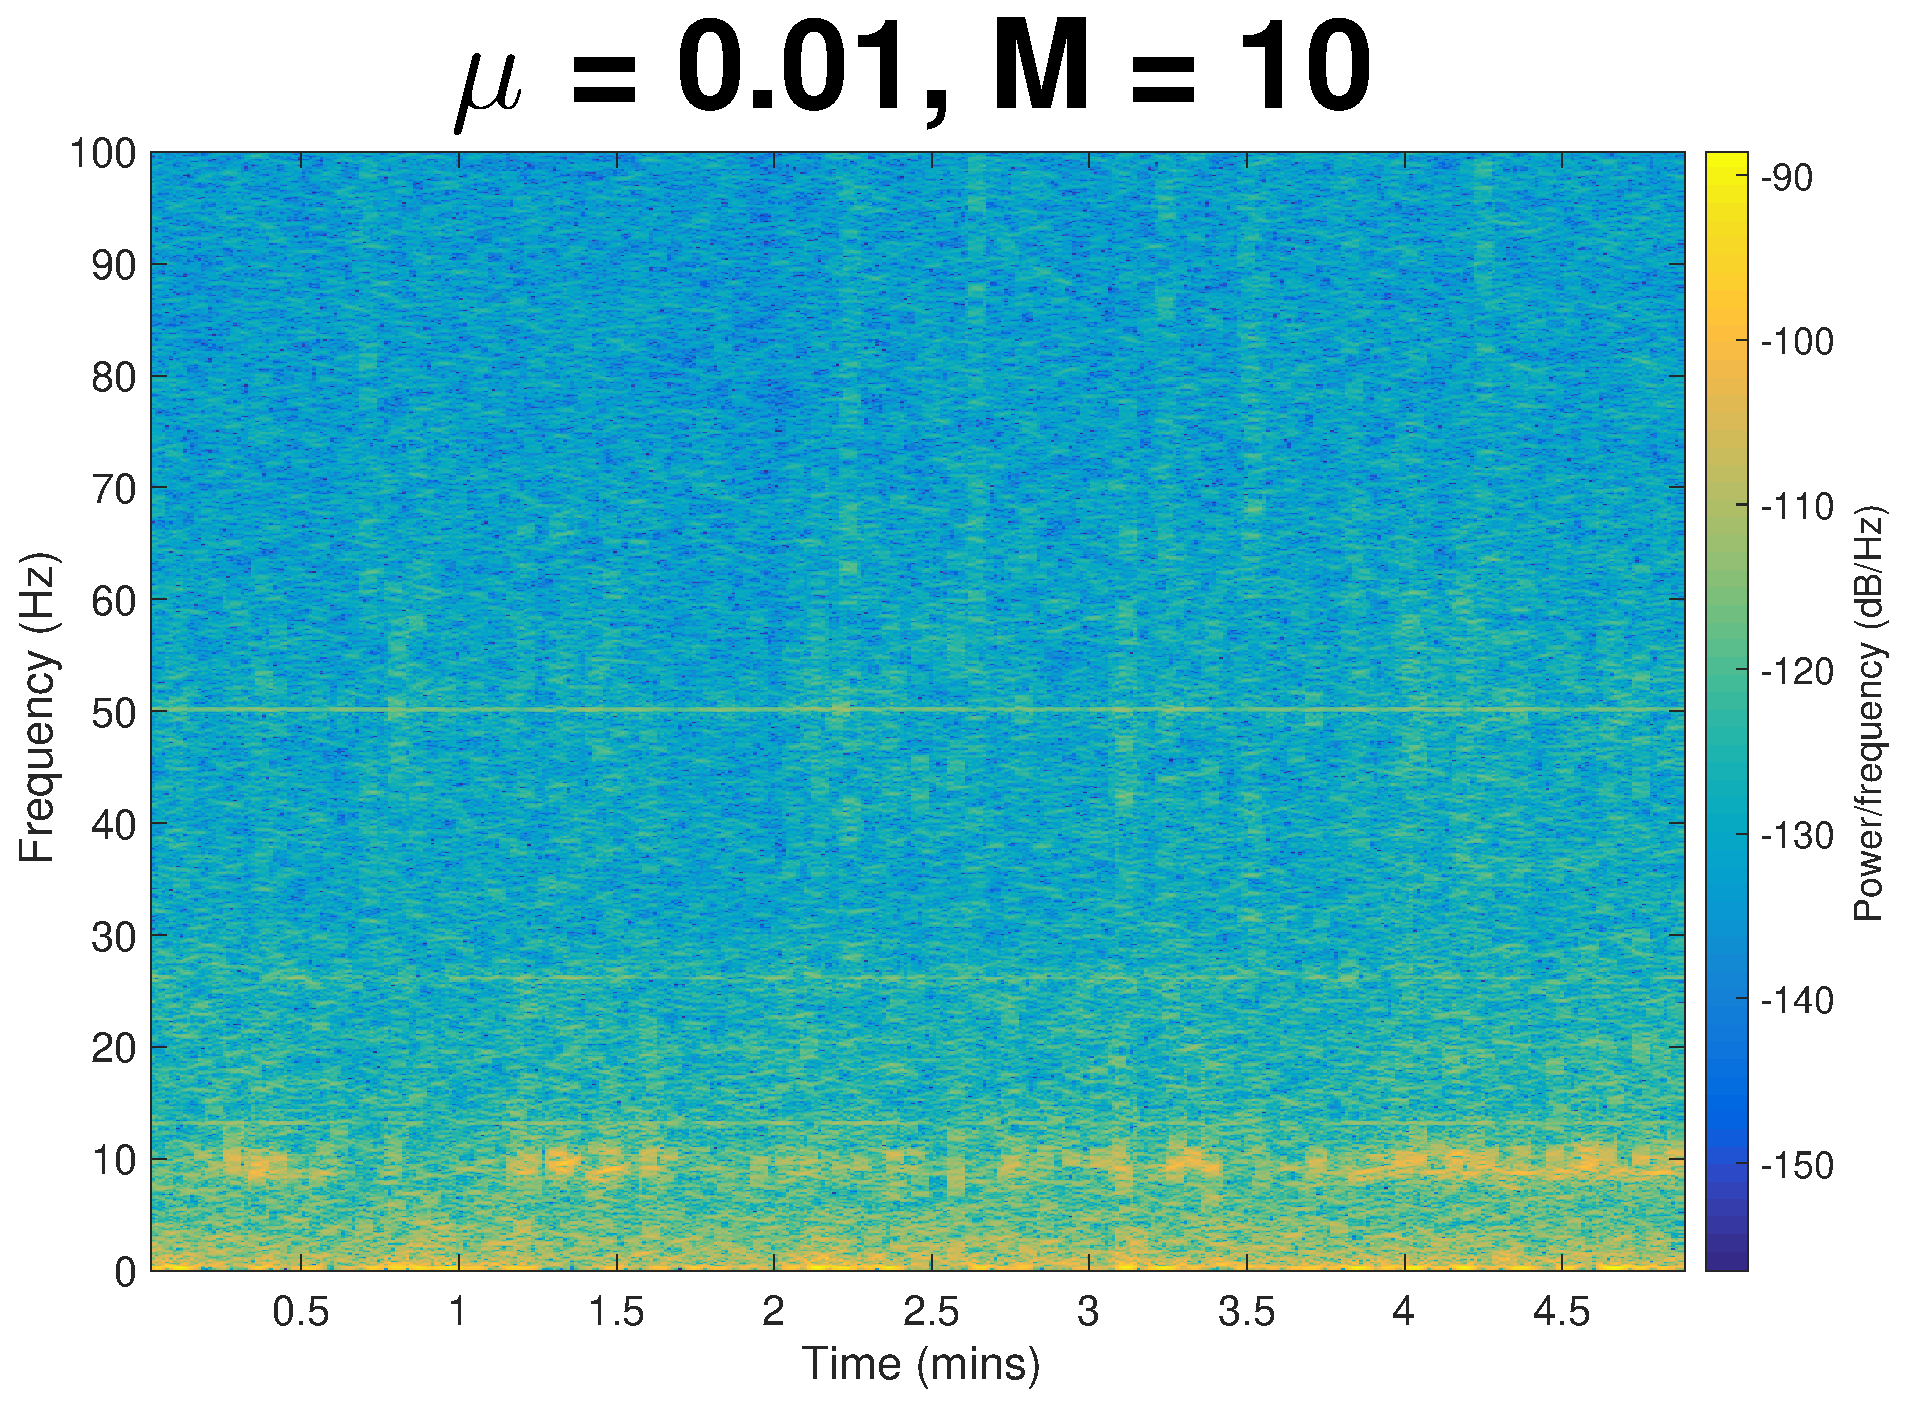
\includegraphics[width=0.24\textwidth]{part3/POz_mu_01_M_10}
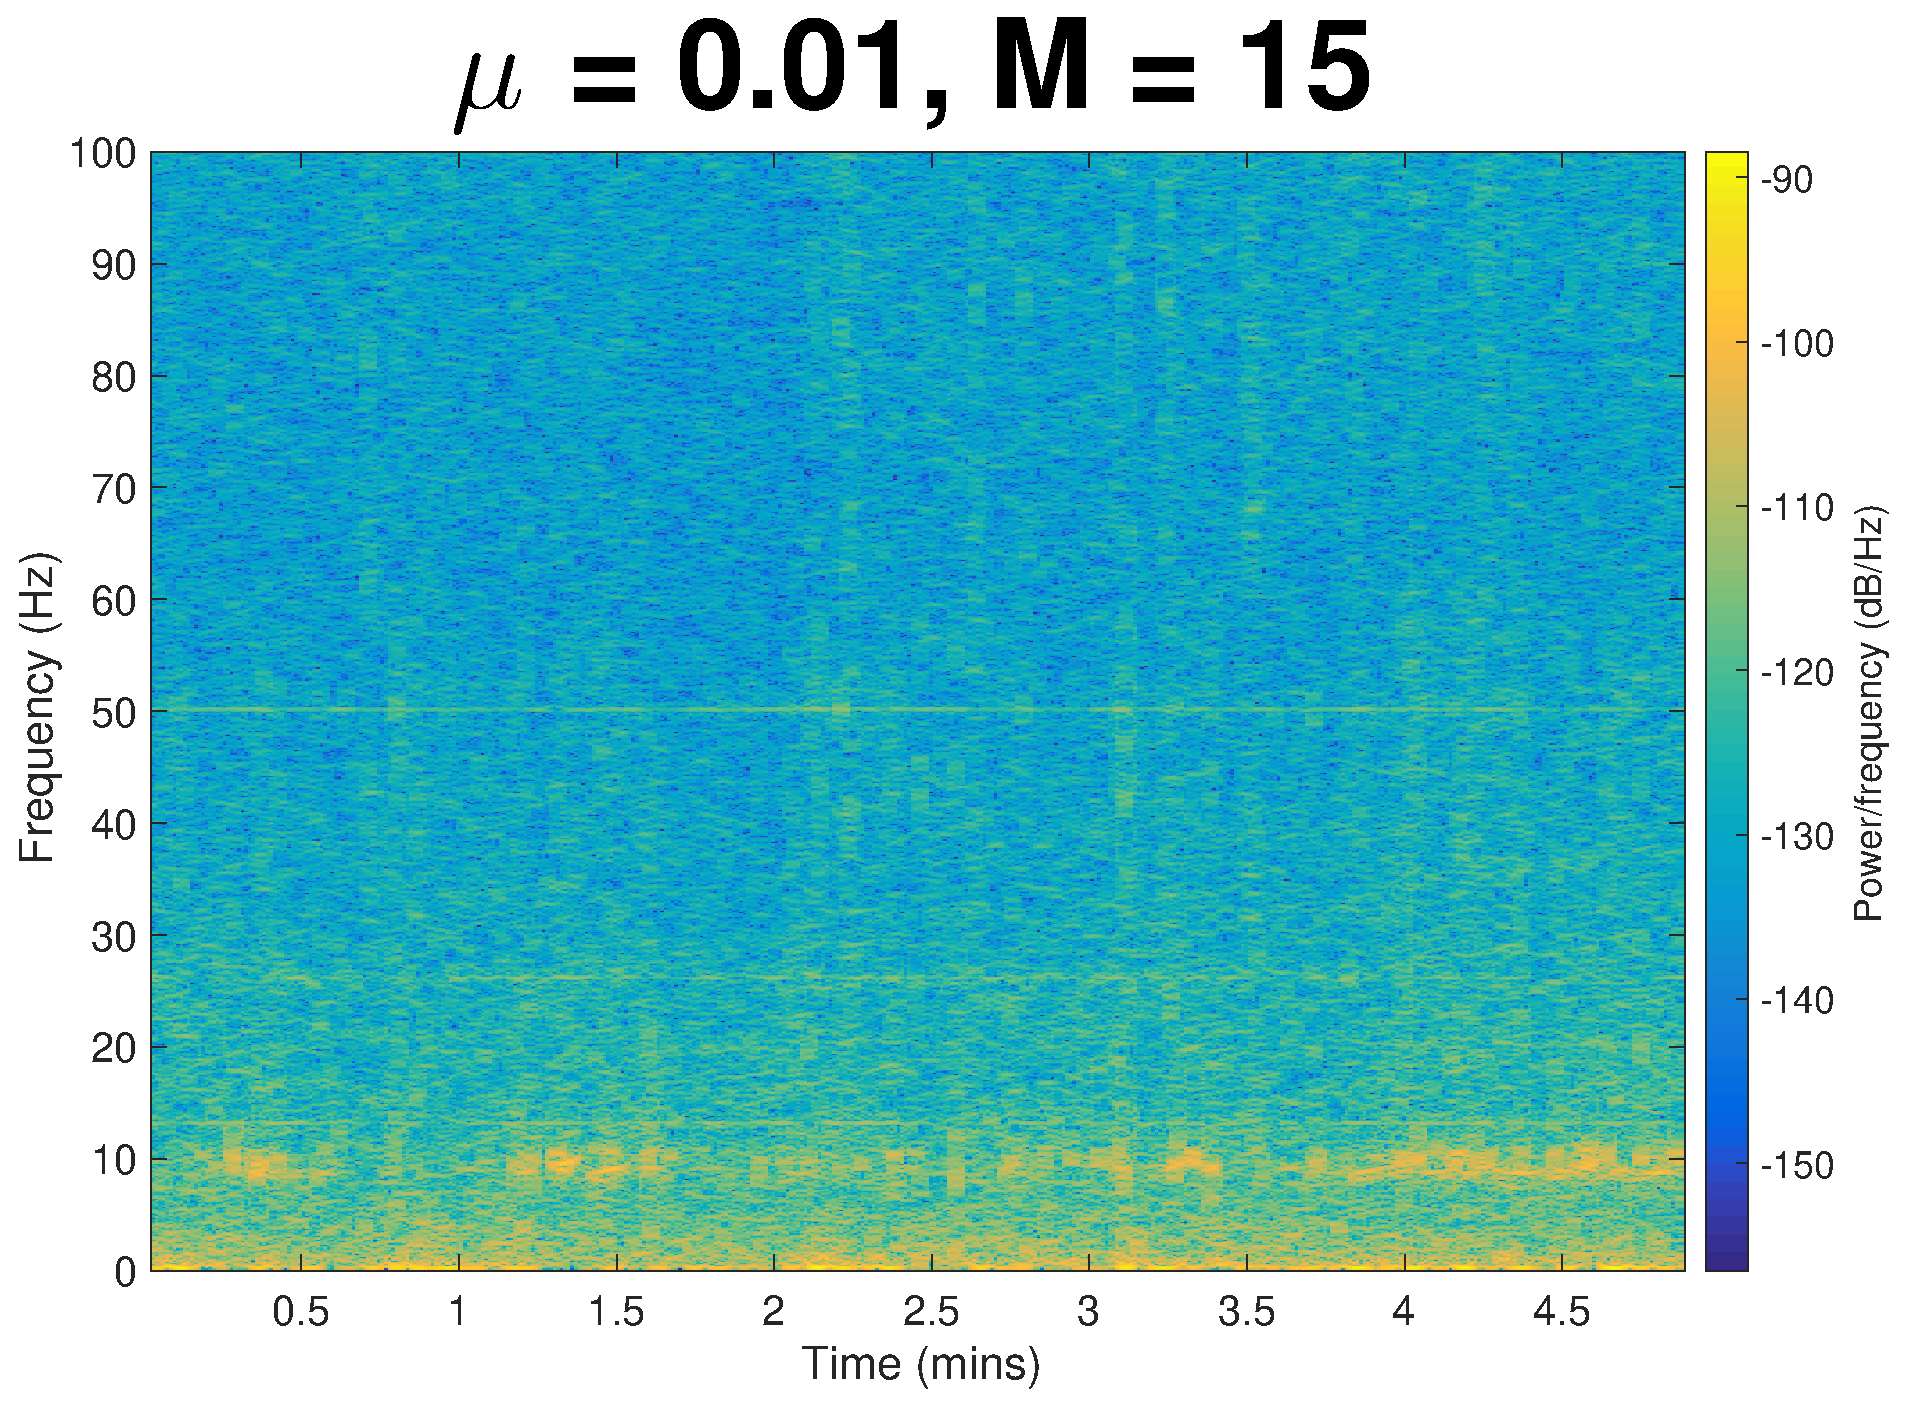
\includegraphics[width=0.24\textwidth]{part3/POz_mu_01_M_15}
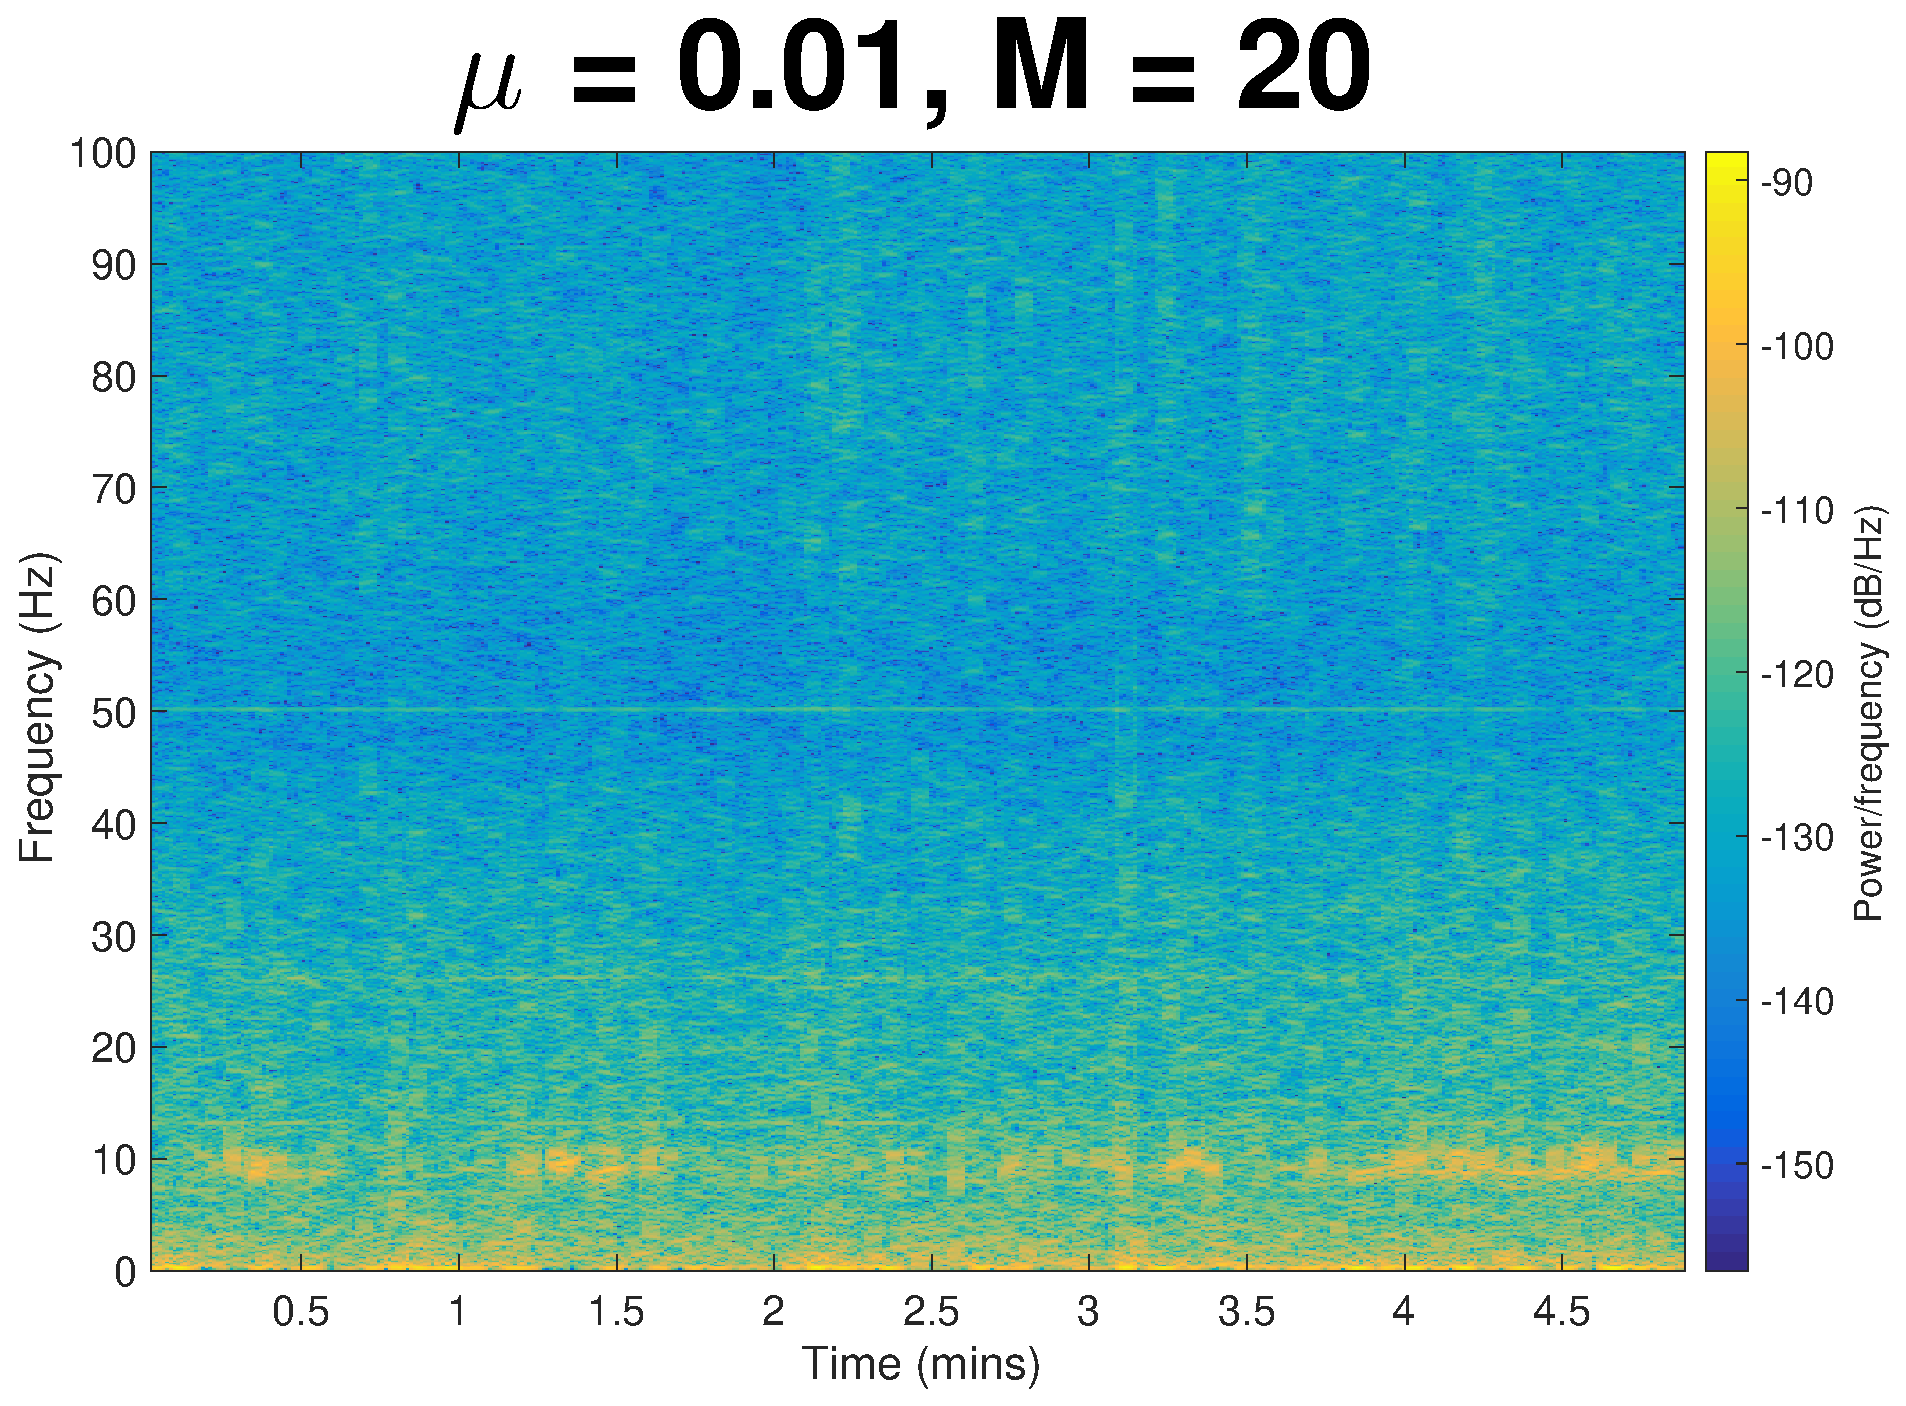
\includegraphics[width=0.24\textwidth]{part3/POz_mu_01_M_20}
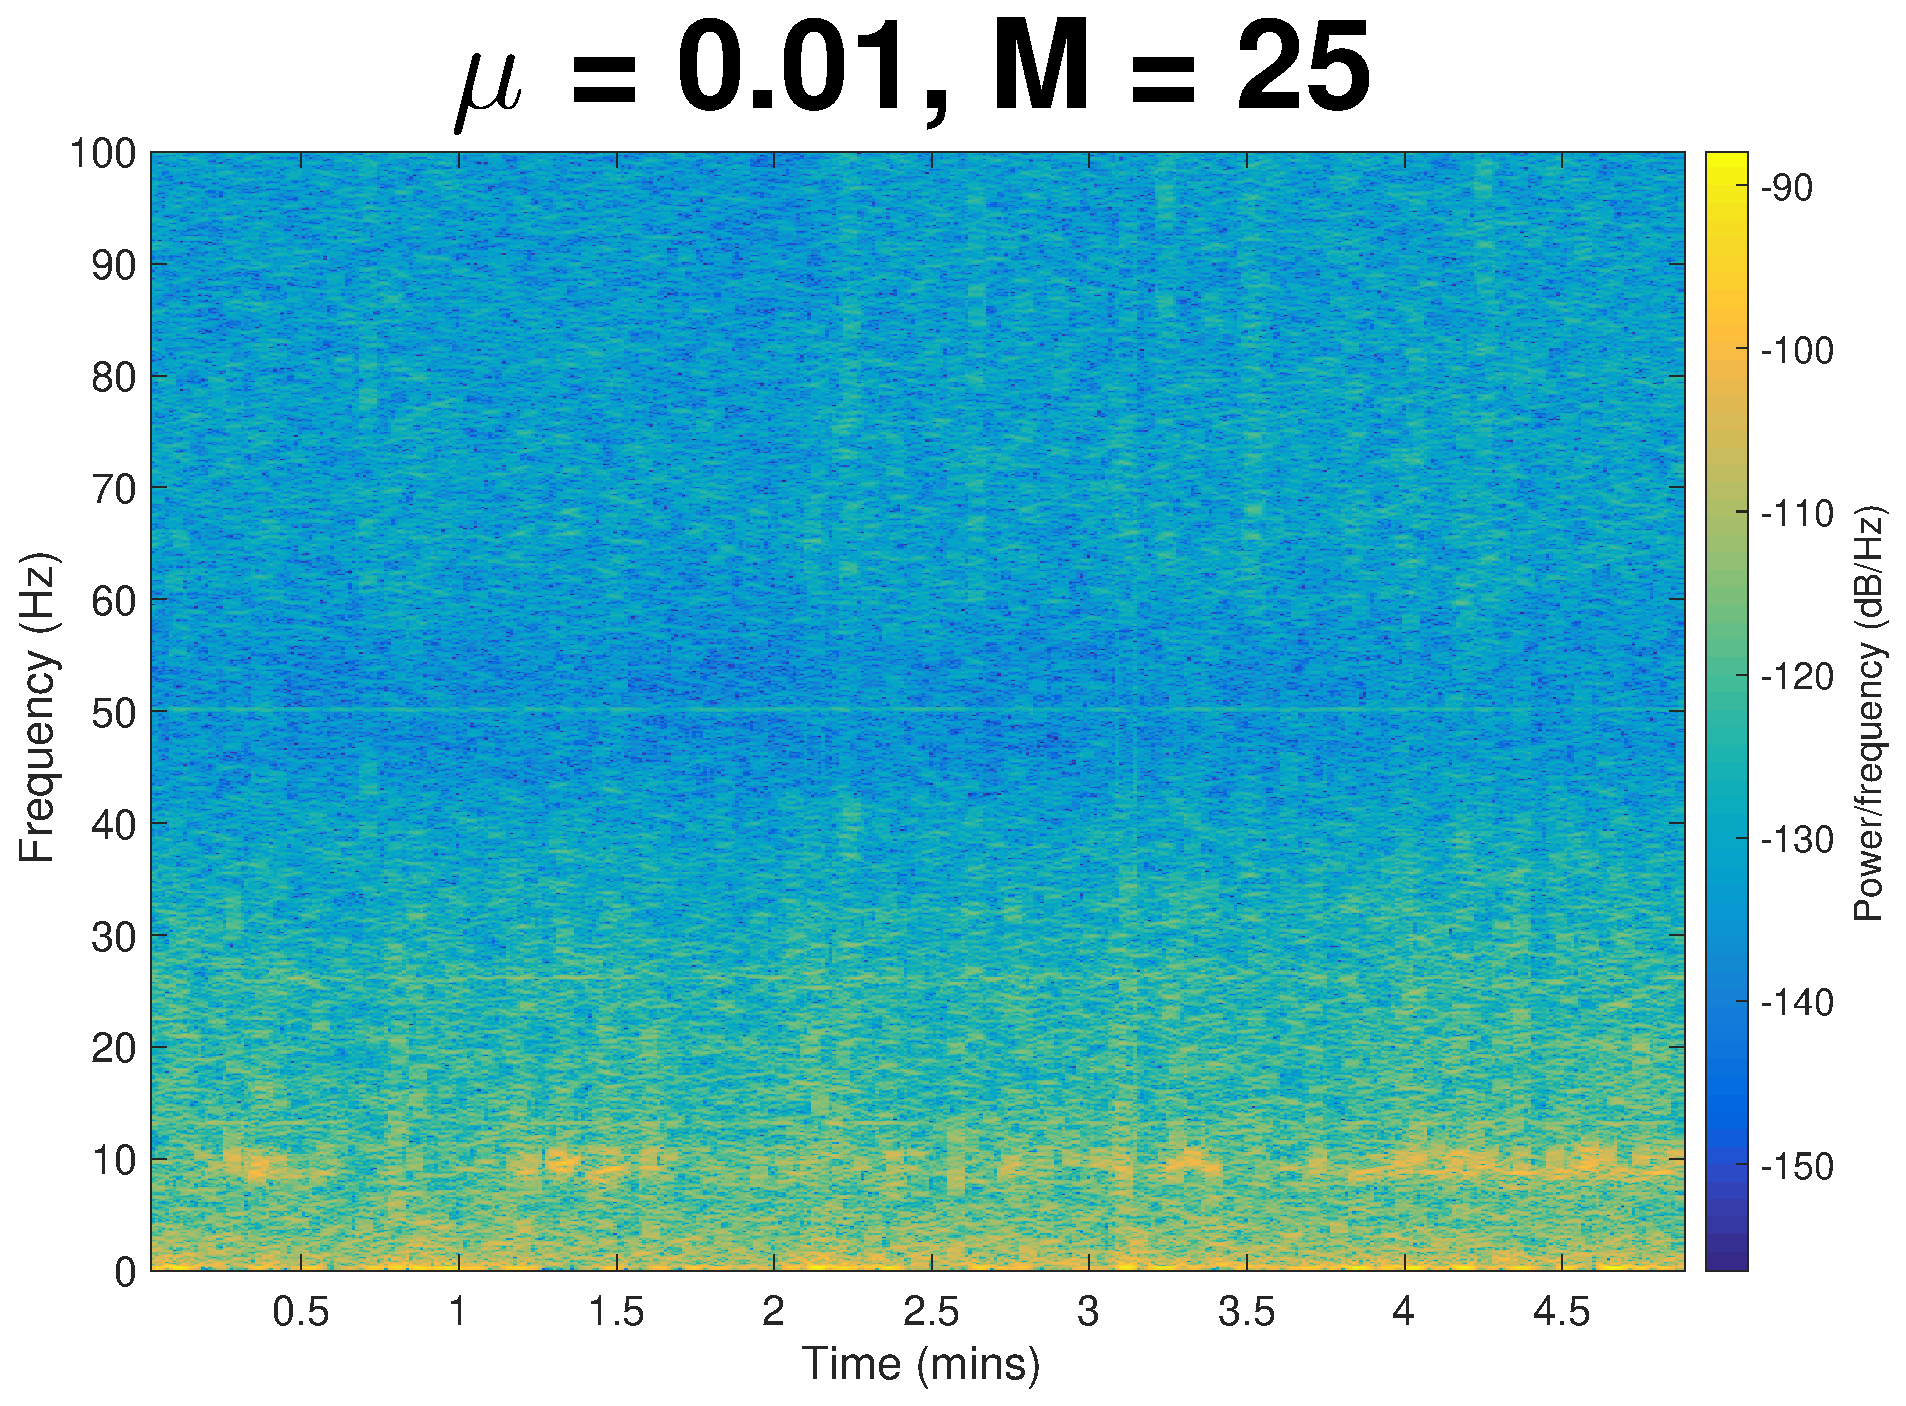
\includegraphics[width=0.24\textwidth]{part3/POz_mu_01_M_25}
\caption{Effect of Increasing Model Order on the Spectrogram of EEG Data}
\end{figure}

\begin{figure}[H]
\centering{}
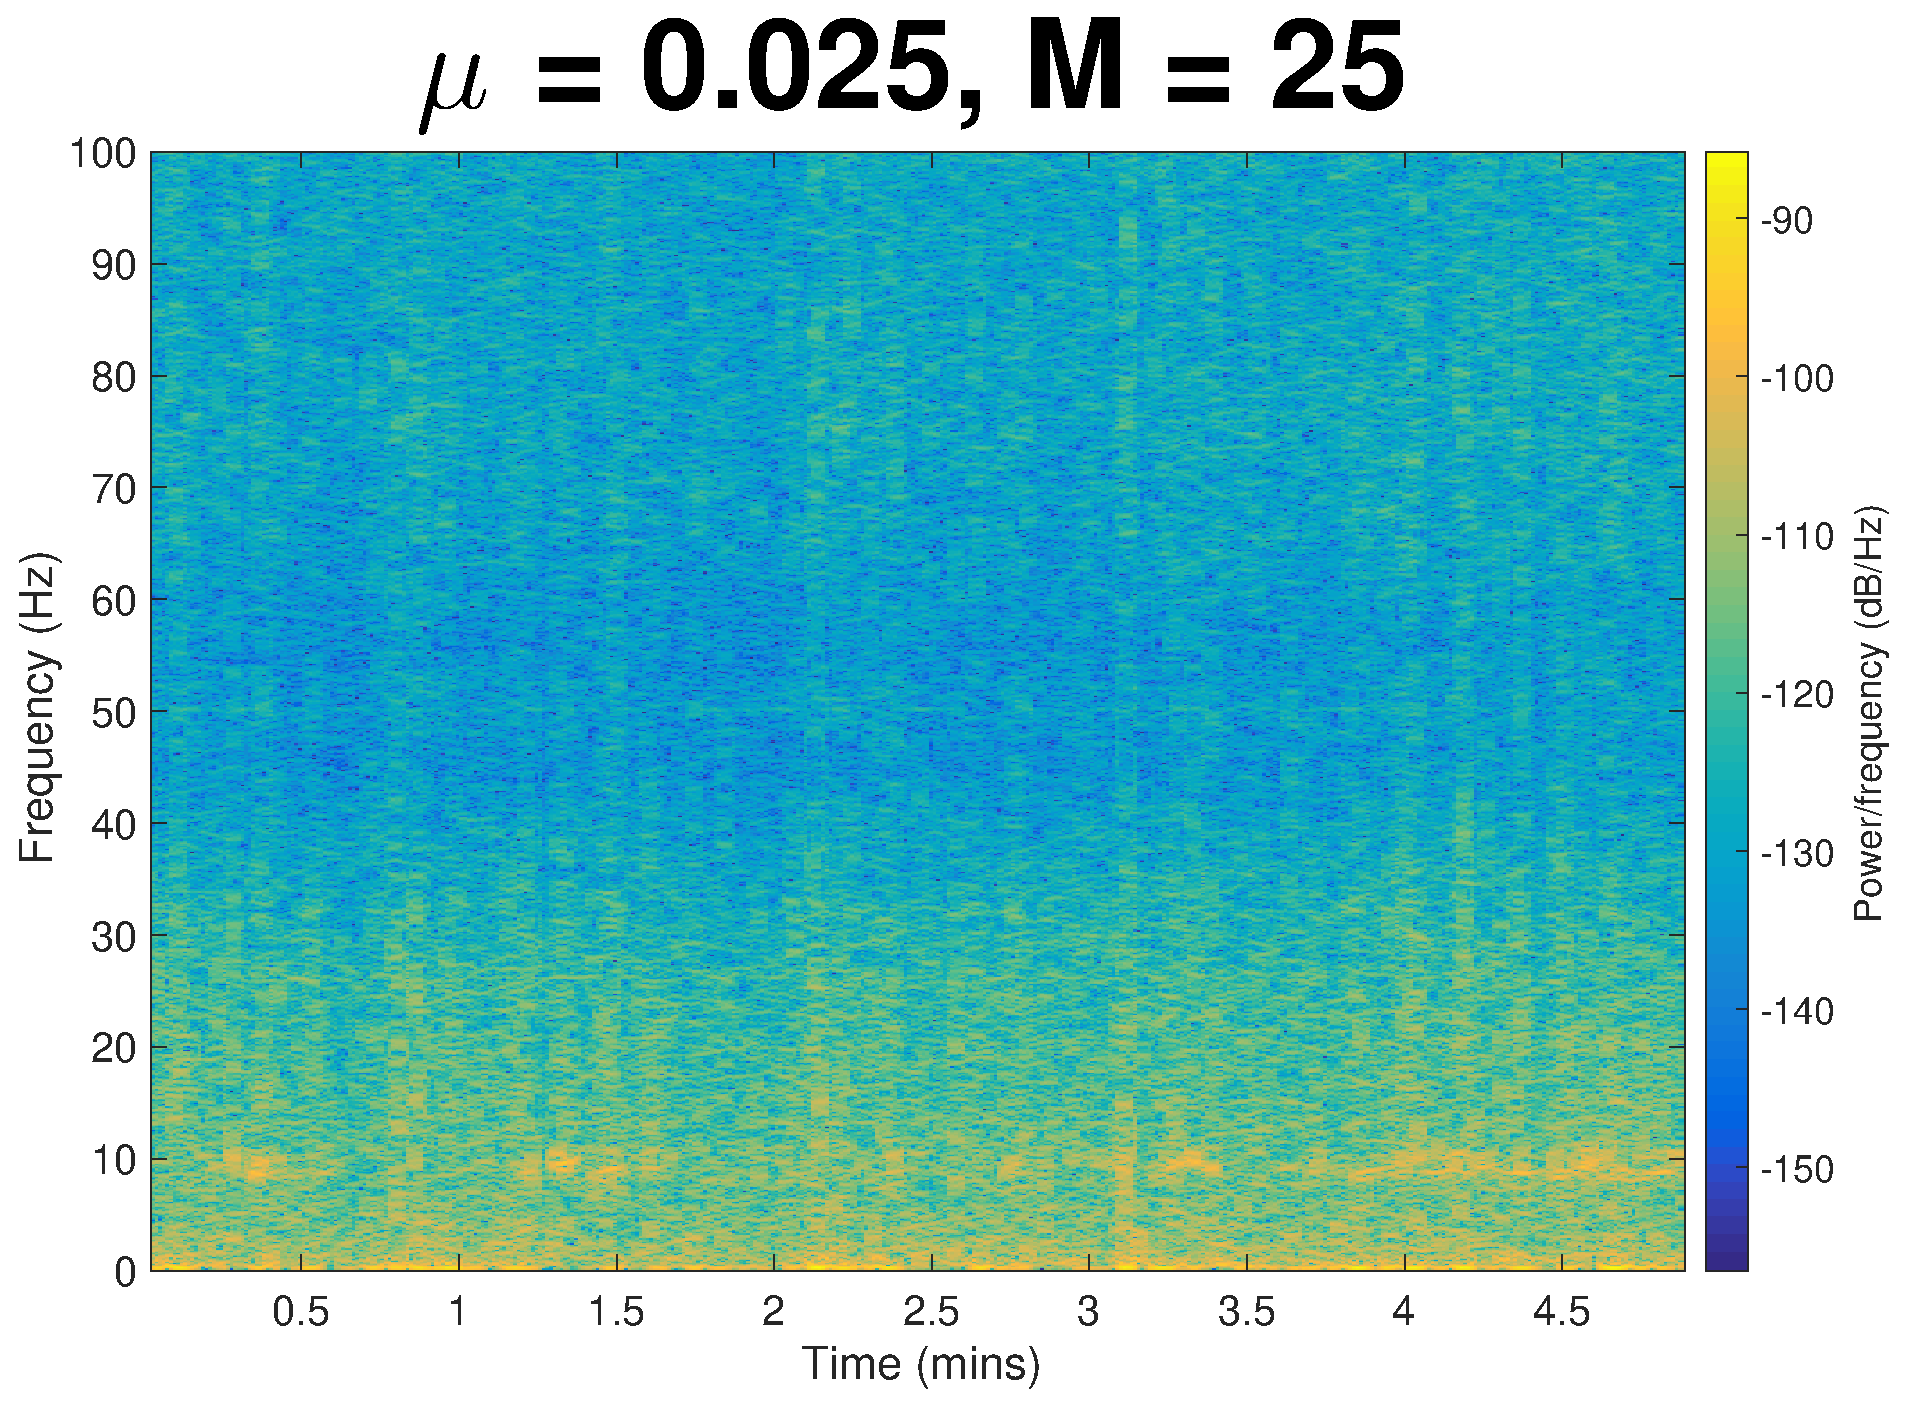
\includegraphics[width=0.24\textwidth]{part3/POz_mu_025_M_25}
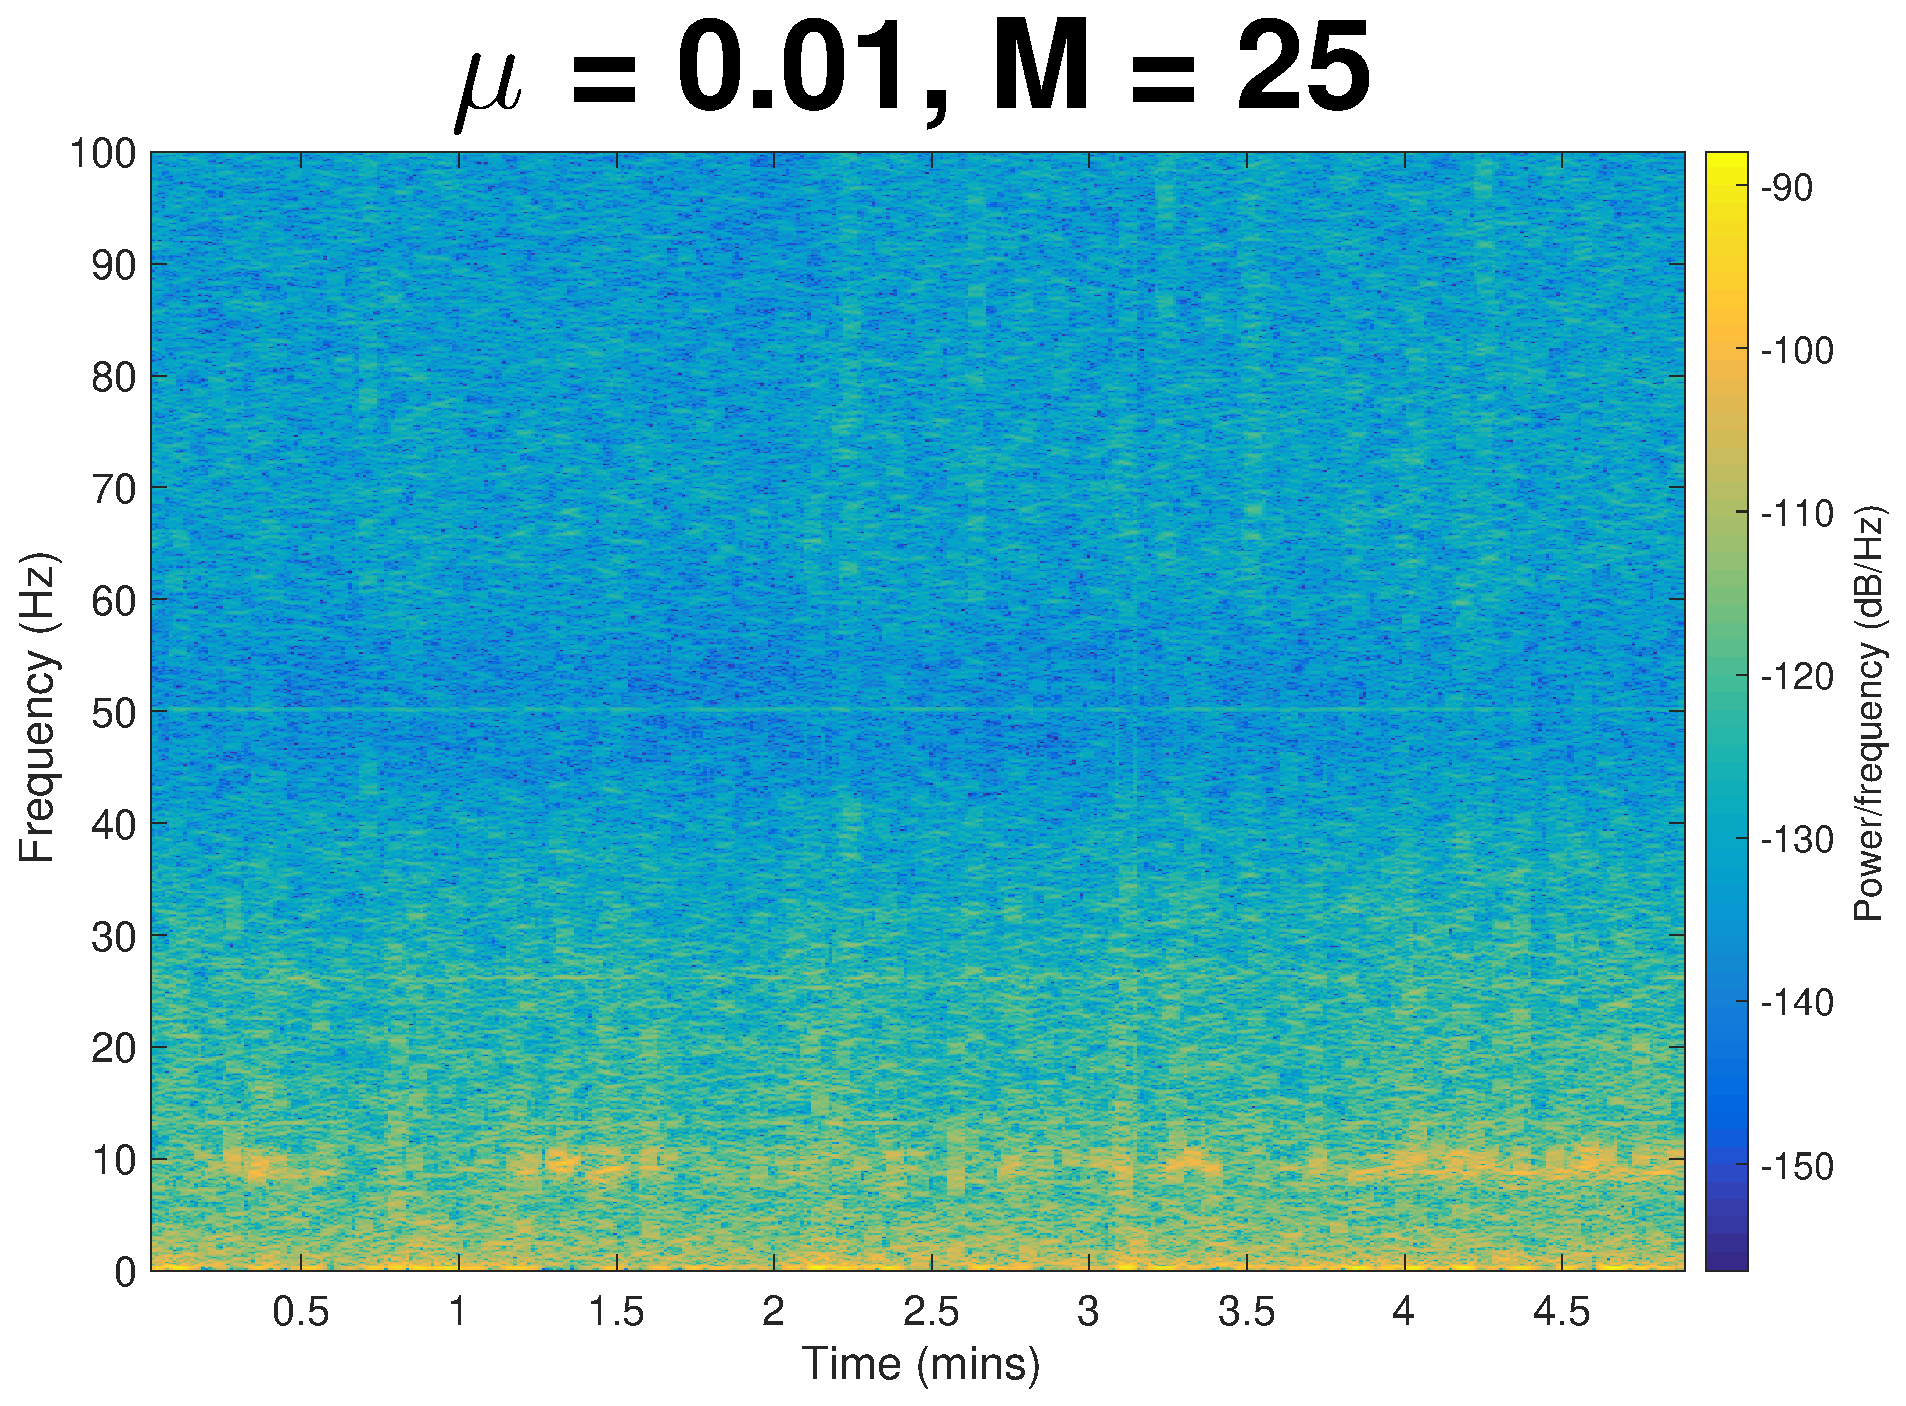
\includegraphics[width=0.24\textwidth]{part3/POz_mu_01_M_25}
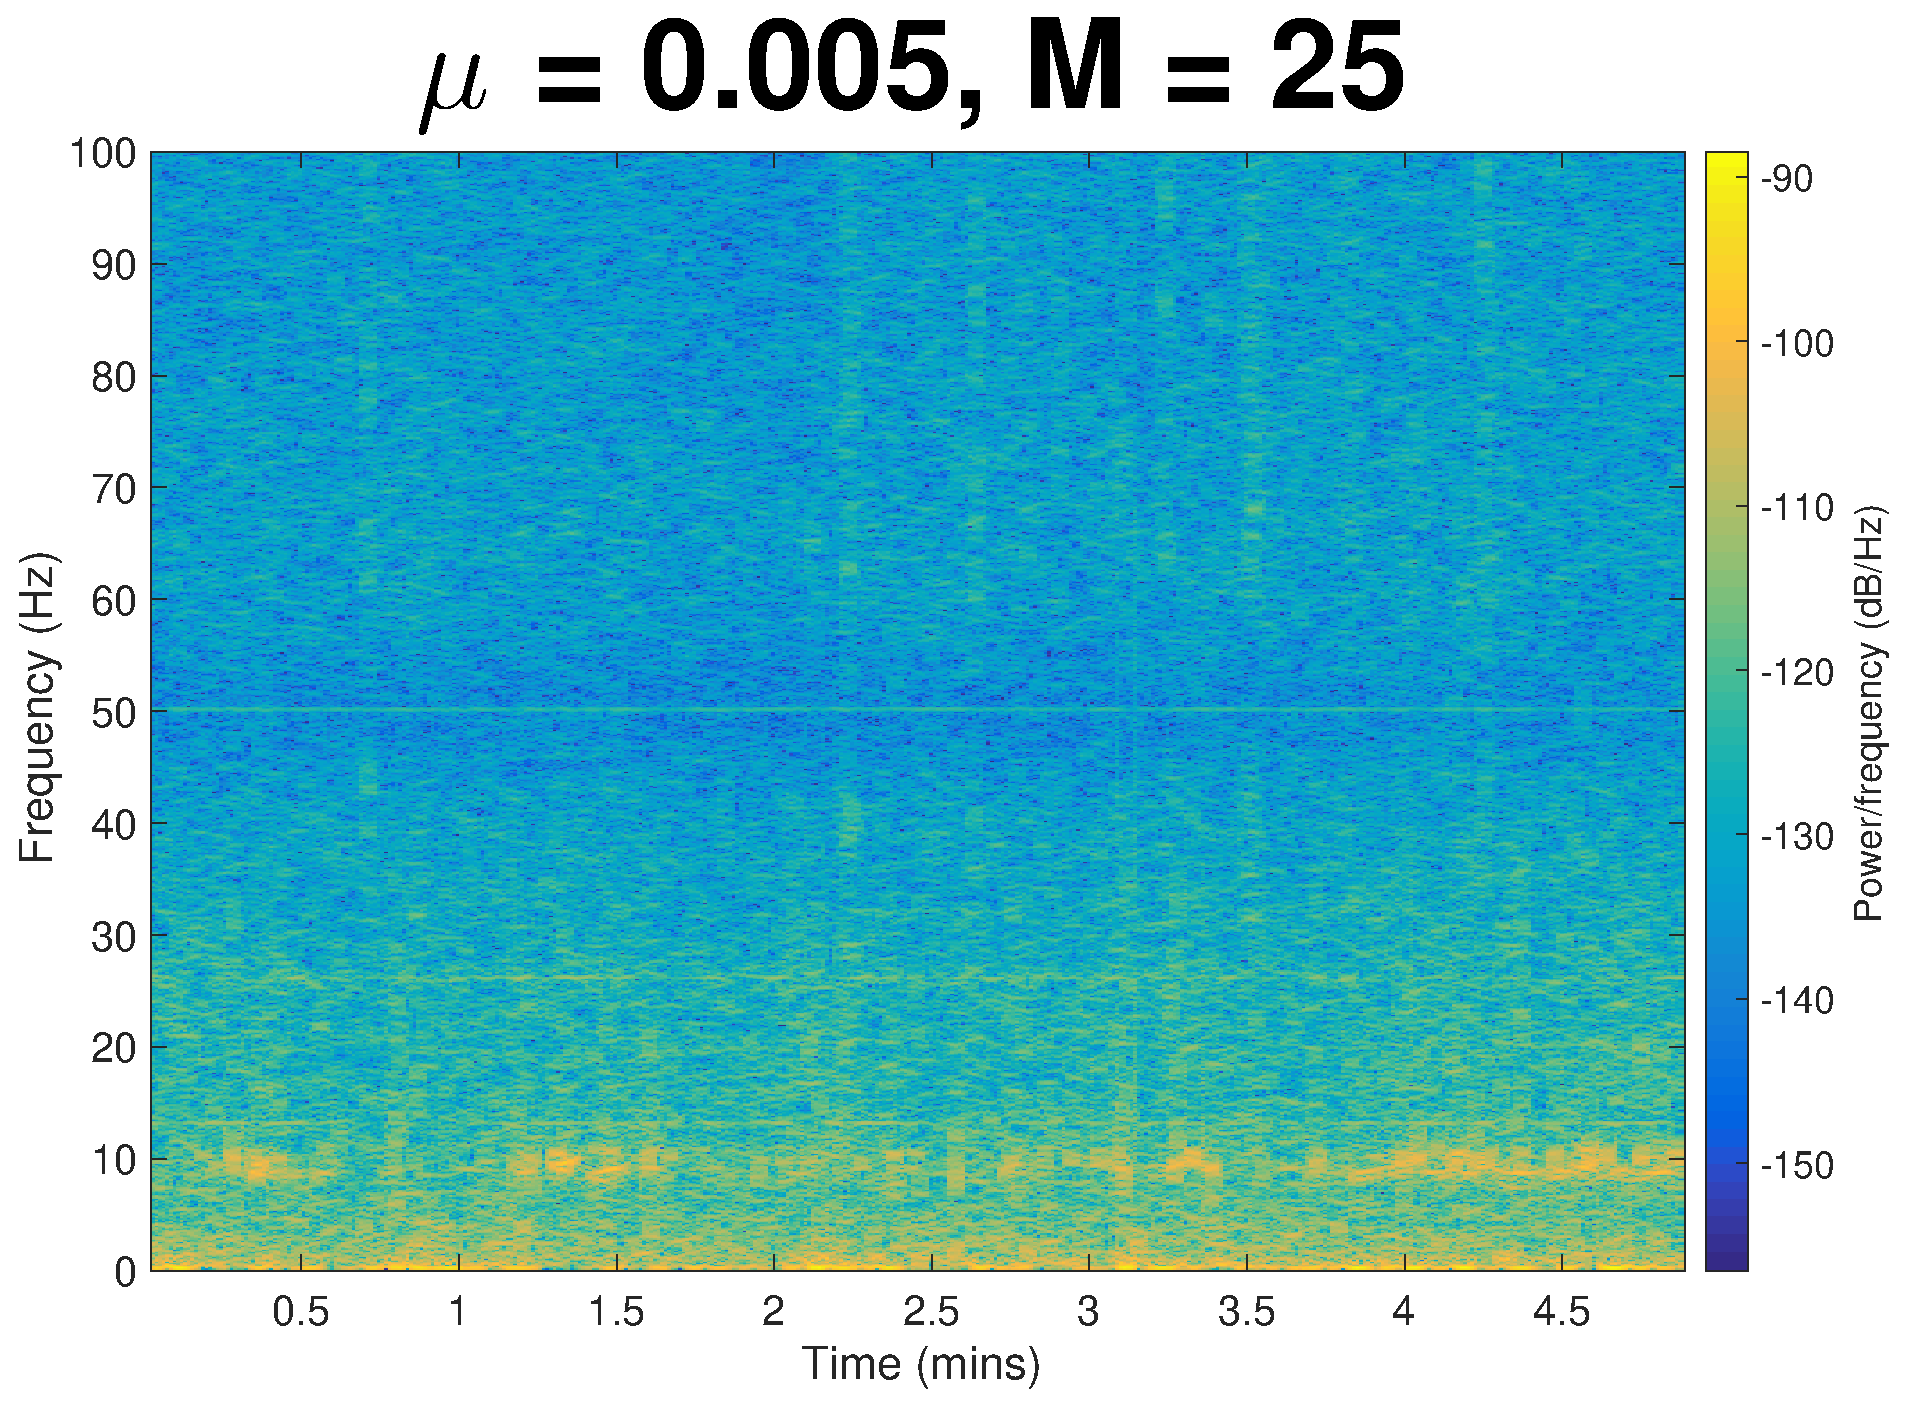
\includegraphics[width=0.24\textwidth]{part3/POz_mu_005_M_25}
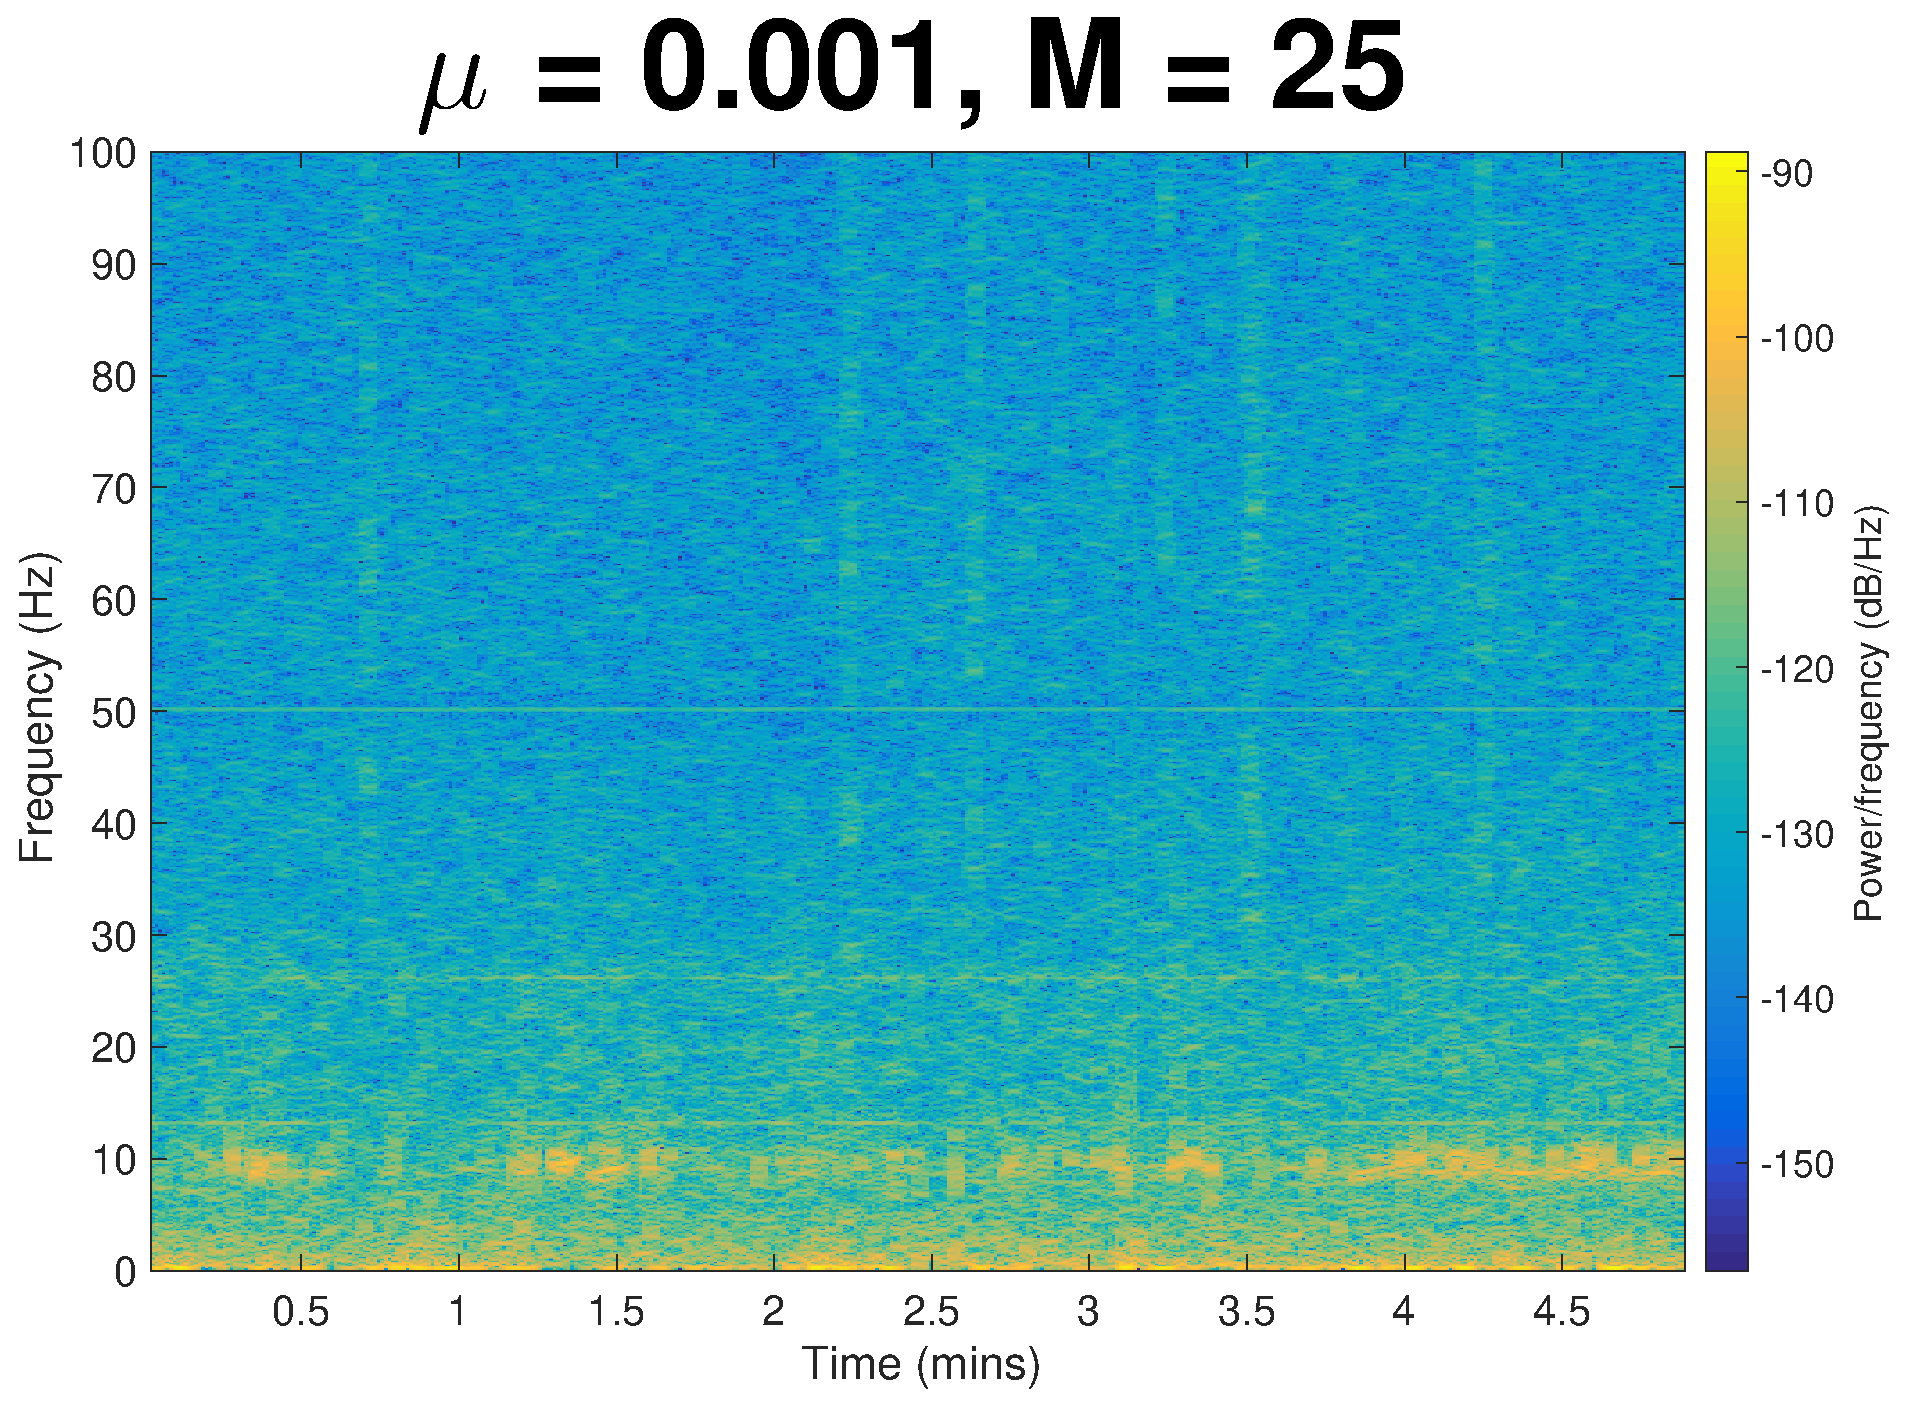
\includegraphics[width=0.24\textwidth]{part3/POz_mu_001_M_25}
\caption{Effect of Varying $\mu$ on the artifacts observed in the Spectrogram of Denoised EEG Data}
\end{figure}


\begin{figure}[H]
\centering{}
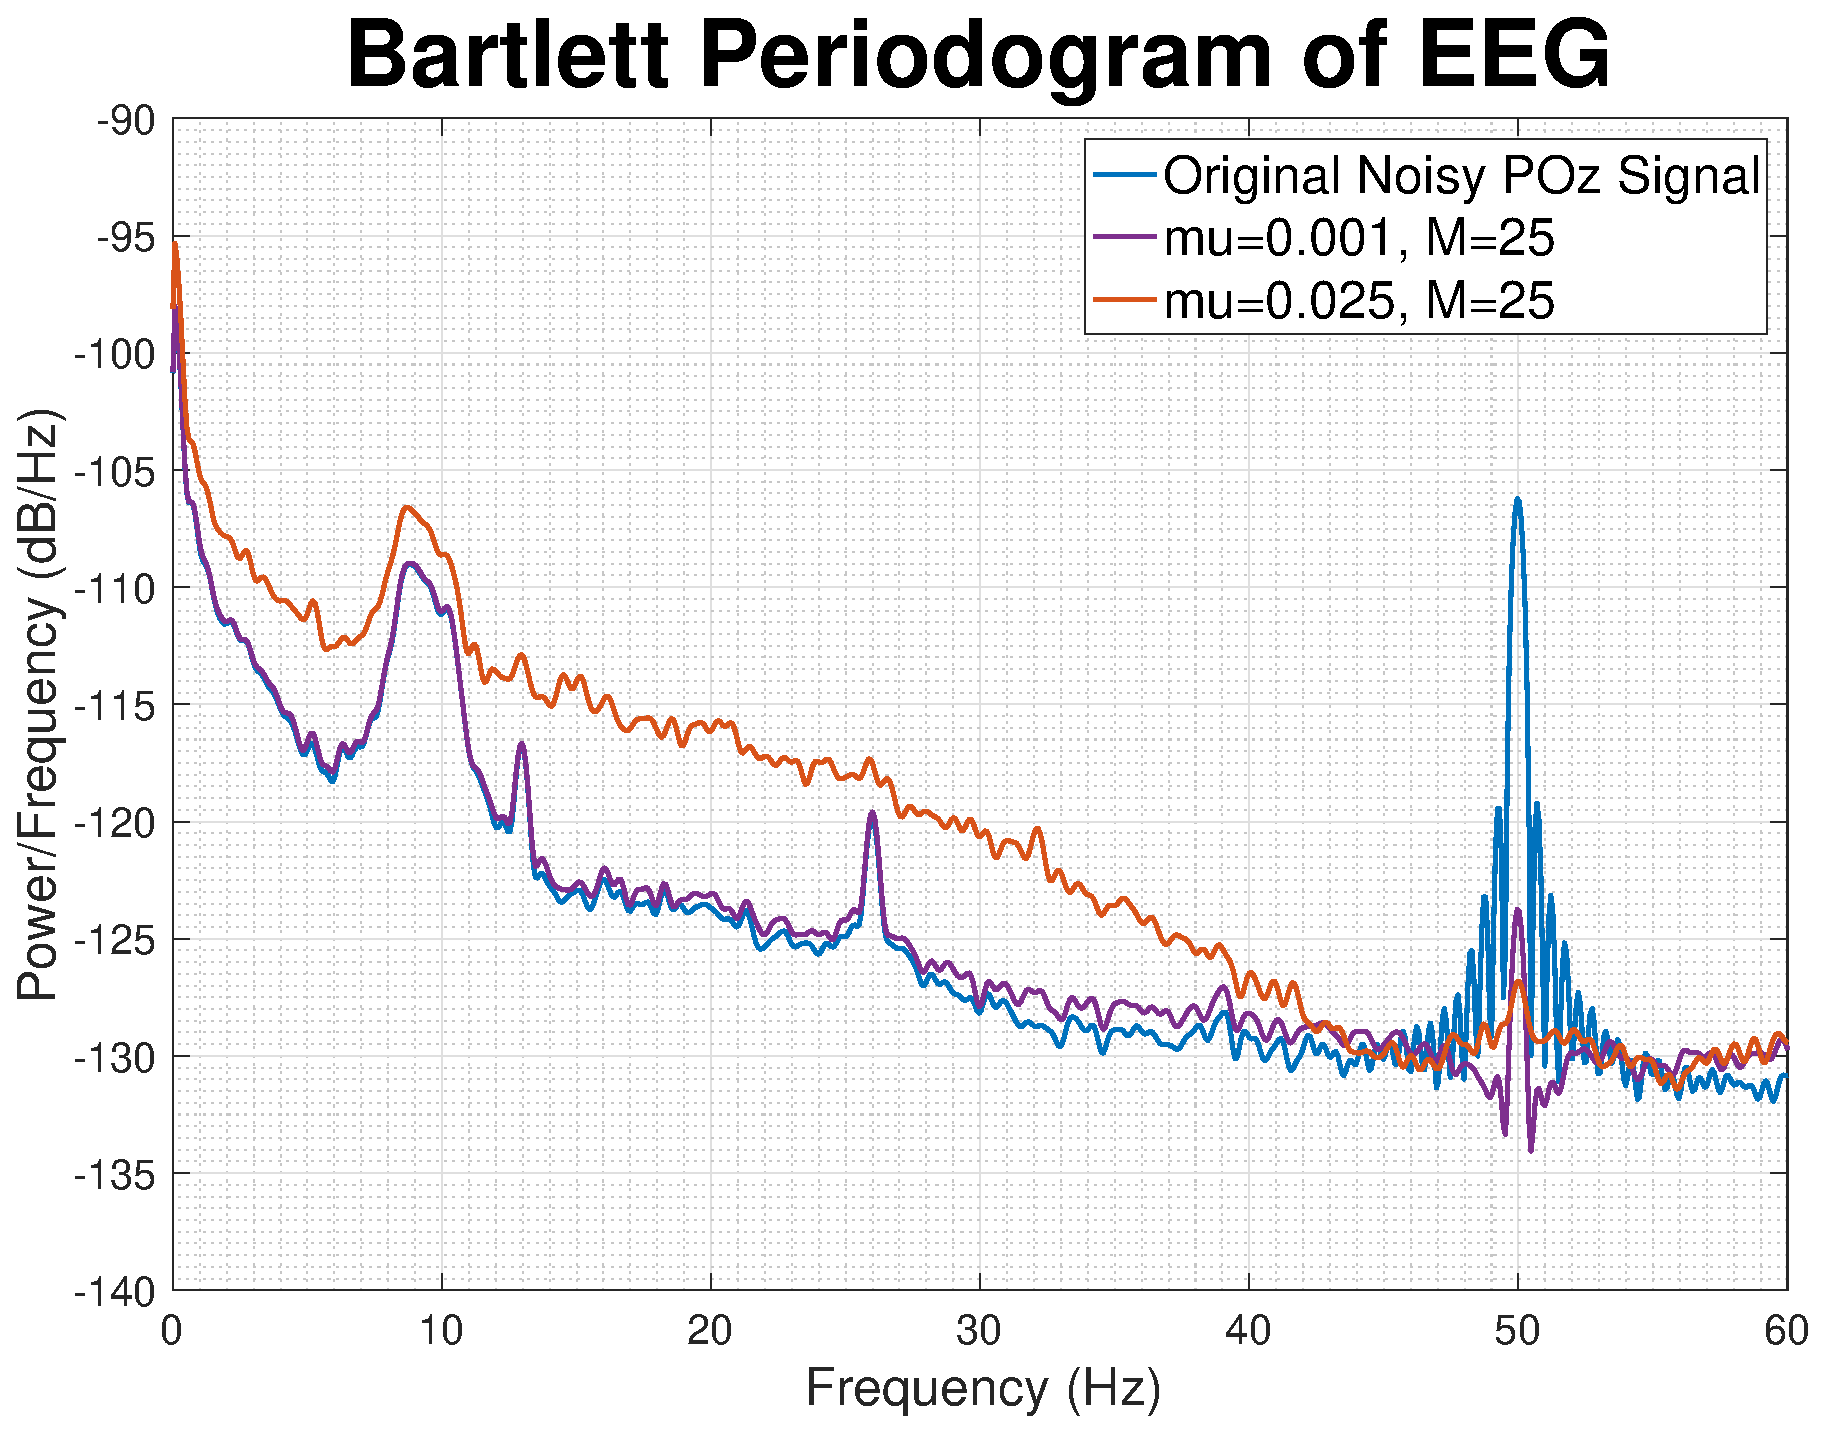
\includegraphics[width=0.32\textwidth]{part3/bartlett_cleaned_Poz}
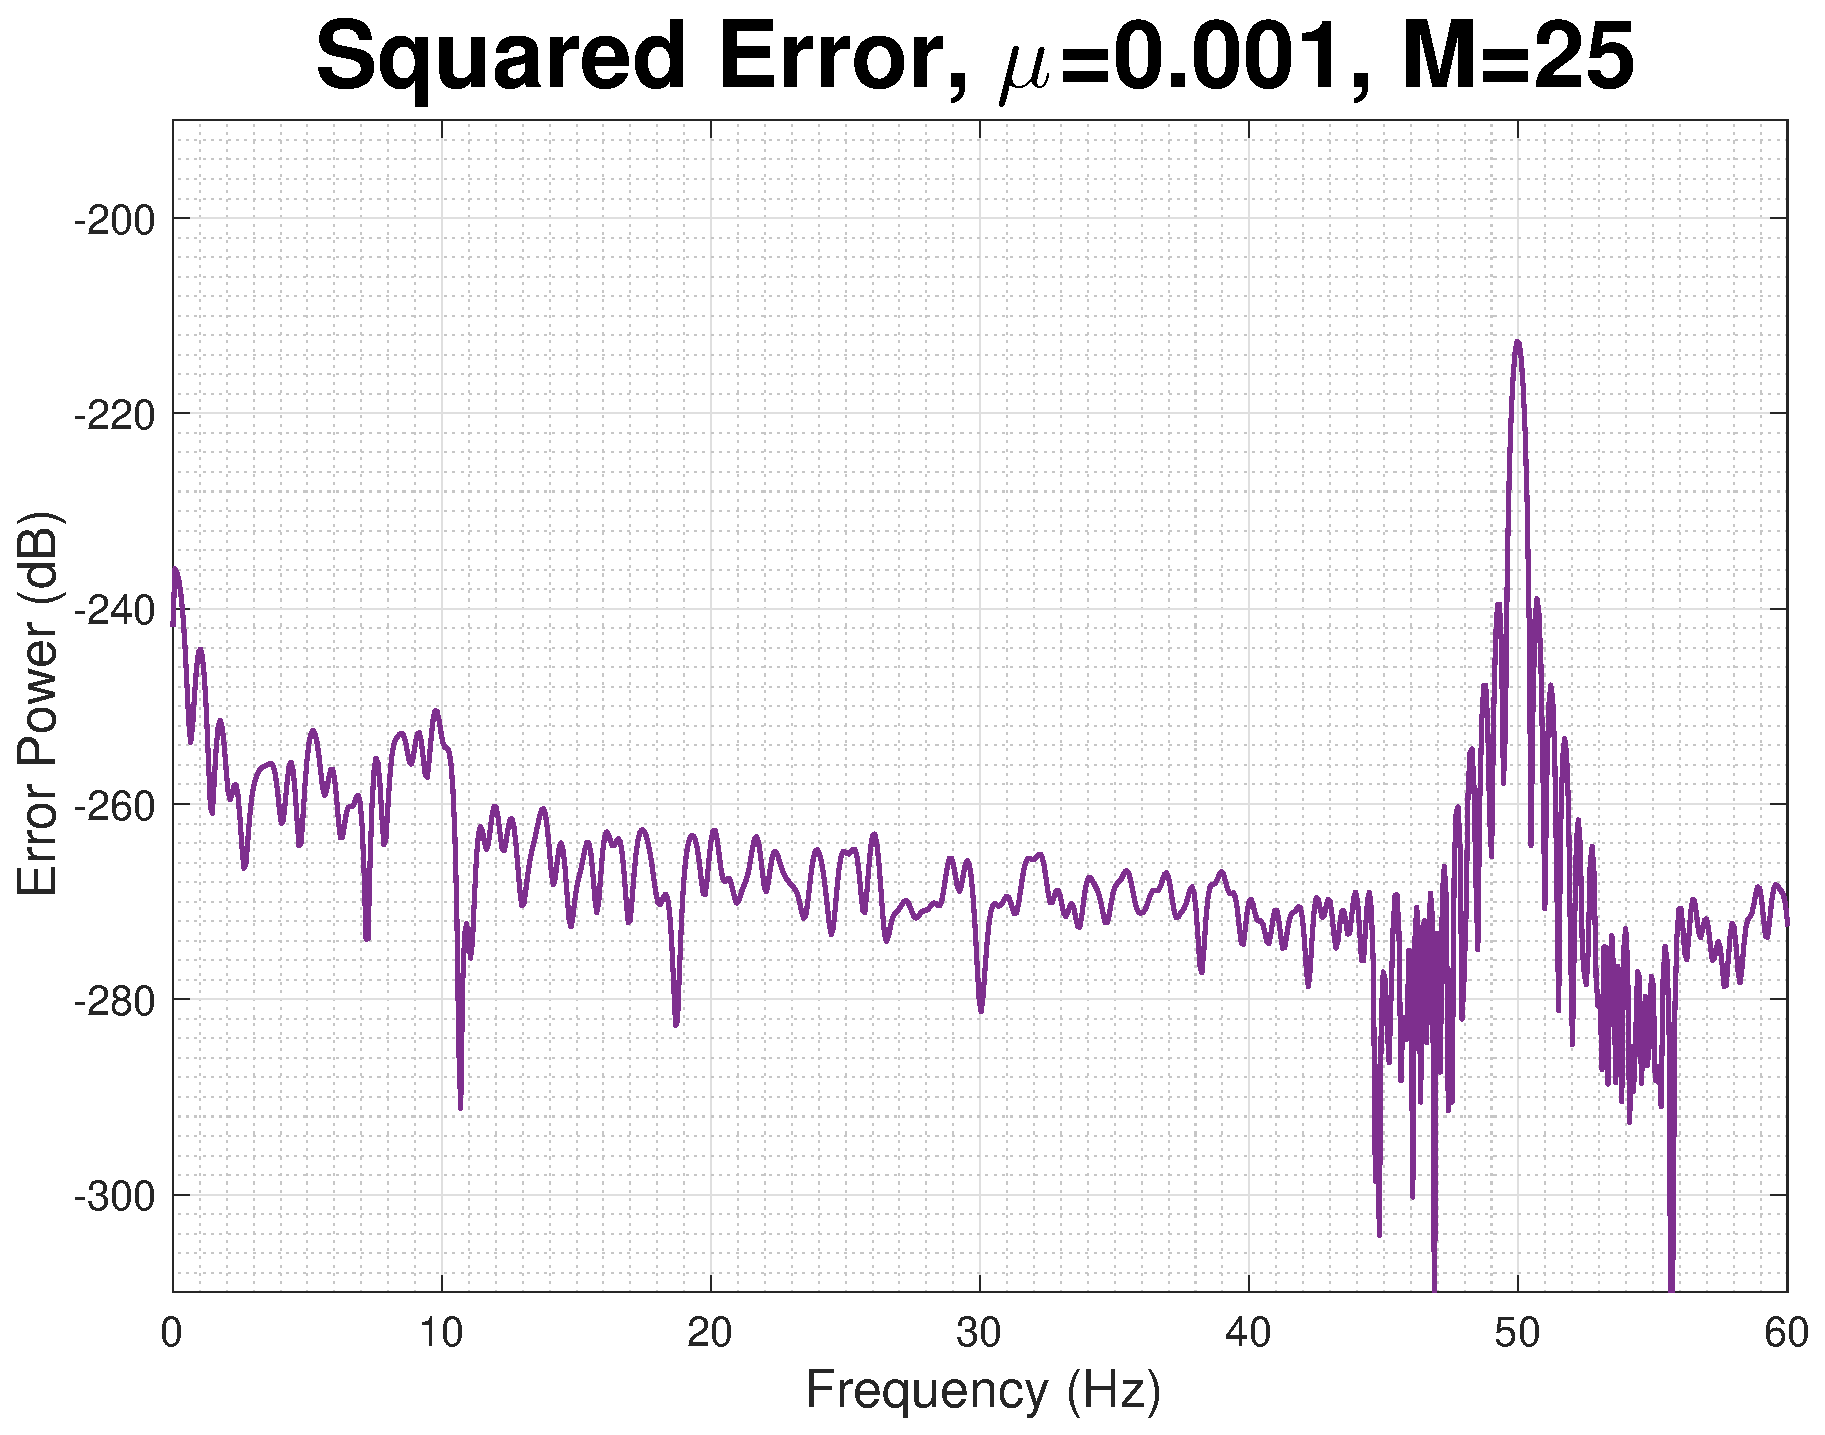
\includegraphics[width=0.32\textwidth]{part3/squared_error_periodogram}
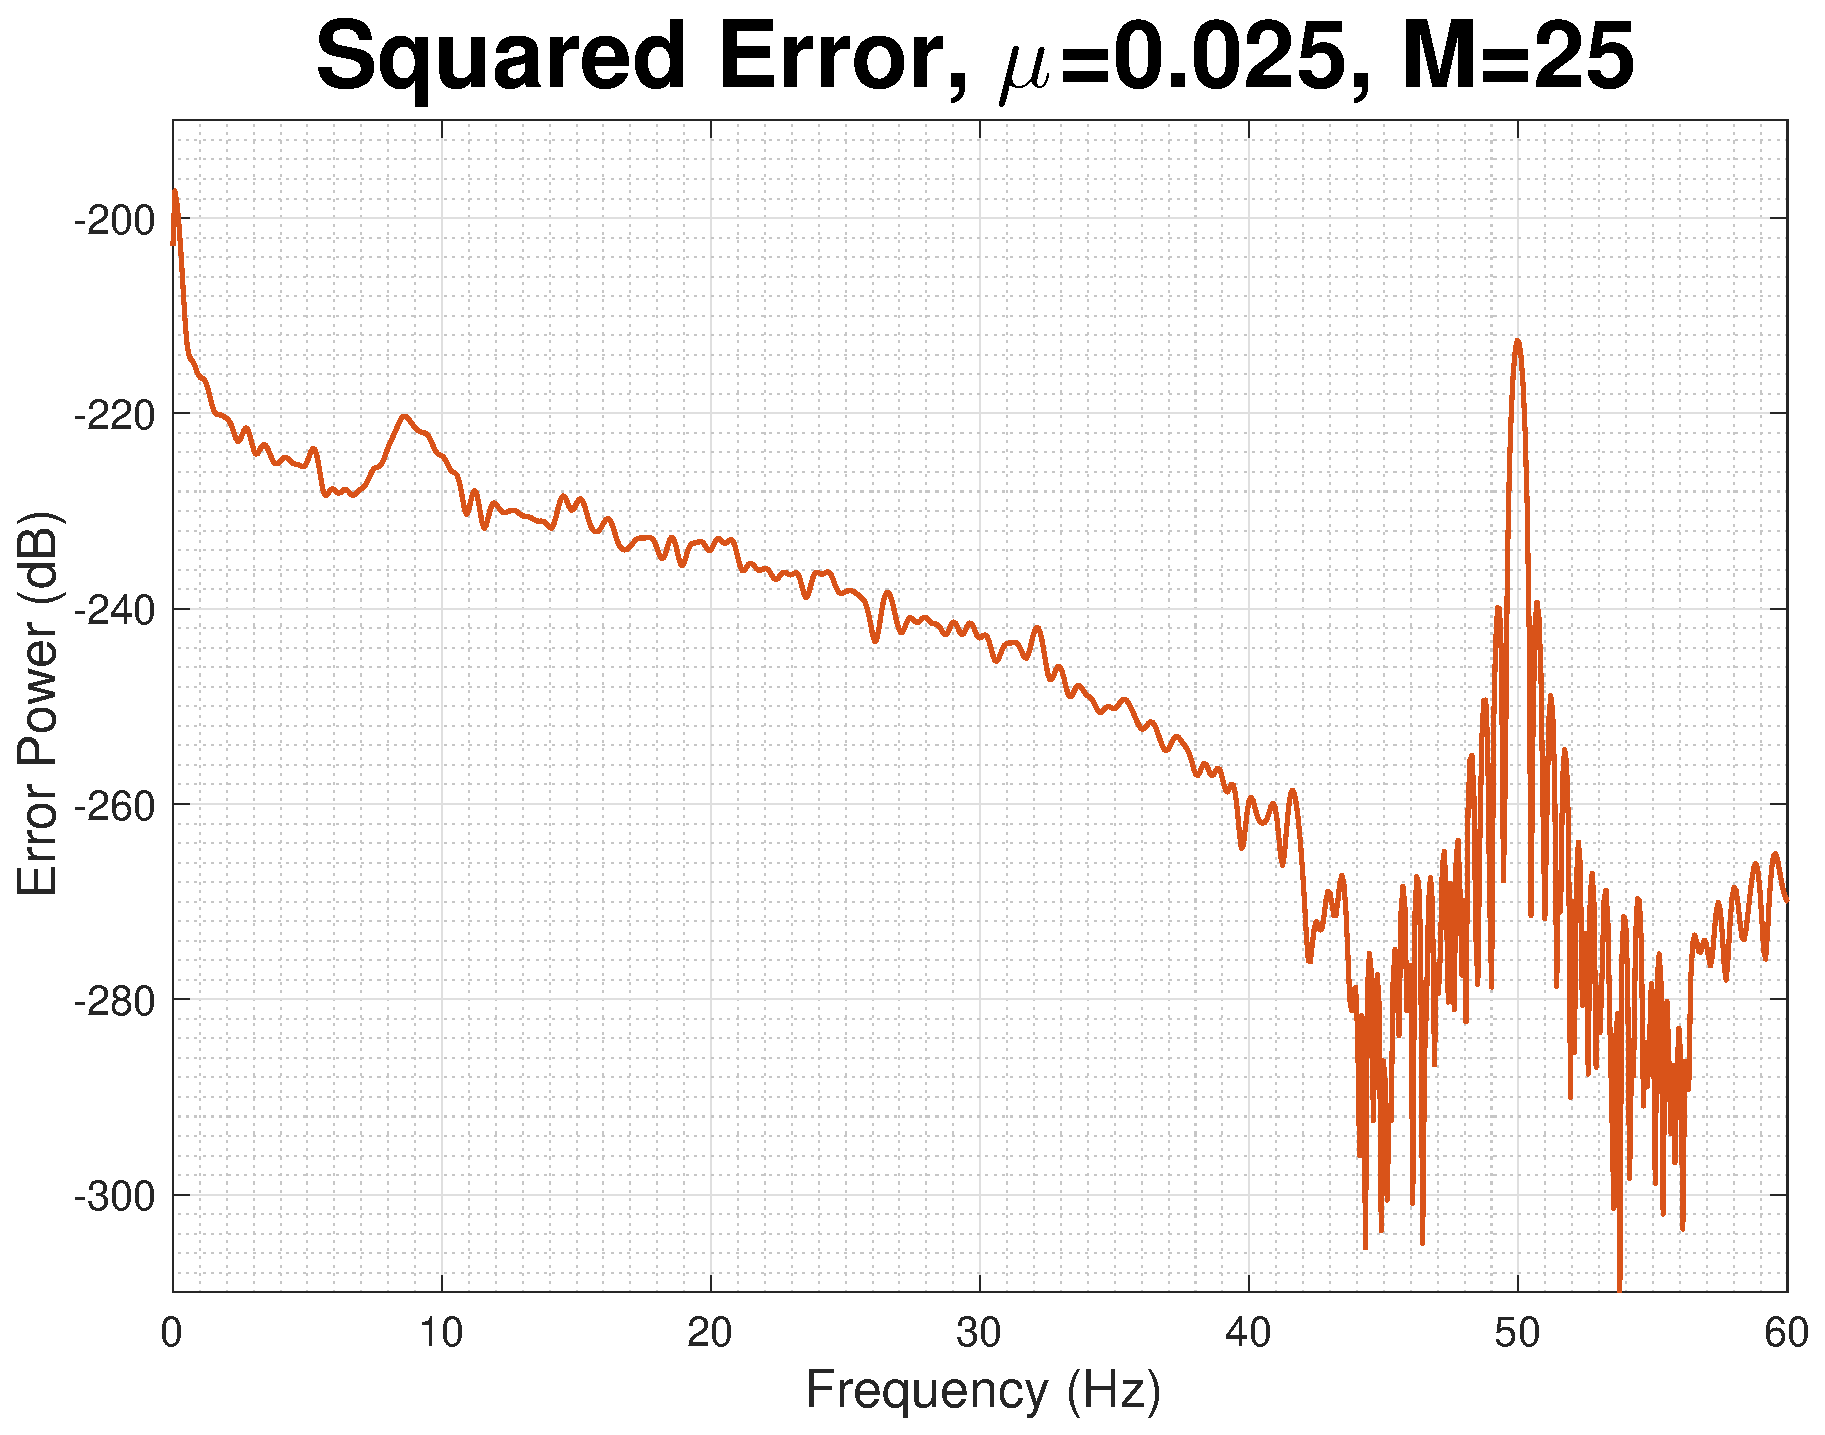
\includegraphics[width=0.32\textwidth]{part3/squared_error_periodogram_bad}
\caption{Bartlett Periodogram, averaged over 2 second intervals, and Squared Errors}
\end{figure}
